\capitulo{5}{Aspectos relevantes del desarrollo del proyecto}

\section{Análisis estático de las redes: Bow-tie}

El concepto de \textit{bow-tie} \cite{enwiki:1148363387} hace referencia a una representación gráfica de una red
que exhibe una estructura en forma de corbata. Se trata de una visualización que segmenta
la red en diversas componentes y describe la conectividad existente entre ellas.

\begin{itemize}
    \item \textbf{Número de nodos (Nº nodes):} Indica la cantidad total de nodos o entidades individuales presentes en la red. Cada nodo representa un elemento o entidad específica dentro del contexto de la red.

    \item \textbf{Número de aristas (Nº edges):} Representa la cantidad total de aristas o conexiones existentes entre los nodos de la red. Cada arista denota una relación o interacción entre dos nodos.

    \item \textbf{Primera componente fuertemente conectada (1st SCC):} Constituye una porción de la red en la cual todos los nodos están interconectados mutuamente a través de rutas directas o indirectas. En otras palabras, se establece un camino desde cualquier nodo de esta componente hacia cualquier otro nodo presente en ella.

    \item \textbf{Segunda componente fuertemente conectada (2nd SCC):} Representa otra parte de la red donde todos los nodos se encuentran interconectados de manera mutua, sin embargo, no existen conexiones directas entre los nodos de la primera componente fuertemente conectada y los nodos de esta componente.

    \item \textbf{Componente de entrada (In component):} Corresponde a la sección de la red que abarca todos aquellos nodos desde los cuales se puede trazar al menos una ruta hacia la primera componente fuertemente conectada.

    \item \textbf{Componente de salida (Out component):} Se refiere a la porción de la red que comprende todos los nodos hacia los cuales existe al menos una ruta partiendo desde la primera componente fuertemente conectada.

    \item \textbf{Tubos (Tubes):} Son trayectorias directas que transcurren desde la componente de entrada hacia la componente de salida sin atravesar la primera componente fuertemente conectada. Estos tubos sirven como enlaces entre las componentes de entrada y salida, eludiendo la estructura de la corbata.

    \item \textbf{Tendril de entrada (In tendrils):} Representan aquellos nodos que están conectados a la componente de entrada, pero no forman parte de la primera componente fuertemente conectada ni de los tubos.

    \item \textbf{Tendril de salida (Out tendrils):} Hacen referencia a los nodos que se encuentran conectados a la componente de salida, sin embargo, no forman parte de la primera componente fuertemente conectada ni de los tubos.

    \item \textbf{Desconectados (Disconnected):} Son los nodos que no están conectados a ninguna otra componente de la corbata y no poseen conexiones entrantes o salientes con otros nodos en la red.

\end{itemize}

Las métricas de \textit{Attack} y \textit{Failure} son dos métricas de vulnerabilidad proporcionadas por el modelo de red de OLIVIA. \cite{Seto-Rey20231}

Estos conceptos proporcionan una descripción detallada de la estructura de la red desde la perspectiva del enfoque \textit{bow-tie}, permitiendo identificar las diferentes componentes y su nivel de interconexión.

A continuación se presentan los resultados obtenidos para cada uno de los repositorios de paquetes analizados.

\subsection{Bioconductor y CRAN}

Para el repositorio de \textit{Bioconductor}, sólo tenemos un conjunto de datos obtenidos mediante \textit{Olivia Finder}.

Para el repositorio de \textit{CRAN} tenemos 4 conjuntos de datos. \ref{tab:data_bc_cran}

\begin{itemize}
    \item El primero usa los datos de \textit{Libraries.io} (\textit{Depends} e \textit{Imports}) sin discriminar versiones de paquete, es decir, para un paquete dado tenemos en cuenta todas las dependencias que ha tenido en cada una de sus versiones. Cabe destacar que este punto de vista carece de sentido, pero se ha incluido para comparar los resultados del anterior \textit{TFG} donde no se tuvo en cuenta este aspecto.

    \item El segundo conjunto de datos usa la última versión de cada paquete disponible e incluye las dependencias del tipo (\textit{Depends} e \textit{Imports}).

    \item El tercer conjunto de datos usa la última versión de cada paquete disponible e incluye las dependencias del tipo (\textit{Depends}, \textit{Imports}, \textit{Suggest} y \textit{Enhances}).

    \item El cuarto conjunto de datos es el obtenido mediante \textit{Olivia Finder} para los tipos de dependencias (\textit{Depends} e \textit{Imports}).
\end{itemize}

\begin{table}[ht!]
    \centering
    \label{tab:data_bc_cran}
    \tiny
    \begin{tabular}{|l|l|l|l|l|l|l|l|l|l|}
        \hline
        \textbf{}              & \textbf{Bioconductor} & \textbf{CRAN}          & \textbf{CRAN}          & \textbf{CRAN}          & \textbf{CRAN}    \\
                               & \textbf{Scraped}      & \textbf{Librariesio 1} & \textbf{Librariesio 2} & \textbf{Librariesio 3} & \textbf{Scraped} \\
        \hline
        \textbf{Nodes (n)}     & 3509                  & 16174                  & 15647                  & 16055                  & 18671            \\
        \textbf{Edges (m)}     & 28320                 & 117724                 & 76207                  & 107370                 & 113273           \\
        \textbf{1st SCC}       & 1                     & 1405                   & 1                      & 923                    & 1                \\
        \textbf{2nd SCC}       & 1                     & 6                      & 1                      & 13                     & 1                \\
        \textbf{In Component}  & 124                   & 381                    & 79                     & 333                    & 6                \\
        \textbf{Out Component} & 0                     & 11746                  & 0                      & 11269                  & 0                \\
        \textbf{Tubes}         & 0                     & 444                    & 0                      & 666                    & 0                \\
        \textbf{In tendrils}   & 2161                  & 1680                   & 14980                  & 2373                   & 17984            \\
        \textbf{Out tendrils}  & 0                     & 481                    & 0                      & 442                    & 0                \\
        \textbf{Disconected}   & 1223                  & 37                     & 587                    & 49                     & 680              \\
        \textbf{Attack}        & 2109                  & 15123                  & 14395                  & 15056                  & 17223            \\
        \textbf{Attack/n}      & 0.6010                & 0.9350                 & 0.9200                 & 0.9378                 & 0.9224           \\
        \textbf{Failure}       & 24.8173               & 1454.5255              & 24.5910                & 957.2135               & 33.5440          \\
        \textbf{Failure/n}     & 0.0071                & 0.0899                 & 0.0016                 & 0.0596                 & 0.0018           \\
        \hline
    \end{tabular}
    \caption{Tabla de datos para Bioconductor y CRAN}
\end{table}

Se ha omitido la columna \textit{CRAN Librariesio 1} en la tabla anterior ya que no aporta información relevante.

\begin{itemize}
    \item \textit{Bioconductor} sigue siendo más pequeño en términos de \textit{nodos} (3509)
          en comparación con las fuentes de \textit{CRAN Librariesio 2}, \textit{CRAN Librariesio 3}
          y \textit{CRAN Scraped}.
    \item En cuanto al número de \textit{aristas} (\textit{edges}), \textit{CRAN Librariesio 3}
          tiene el valor más alto (107,370), seguido de \textit{CRAN Scraped} (113,273) y
          \textit{CRAN Librariesio 2} (76,207).
    \item La cantidad de \textit{nodos} en la \textit{componente fuertemente conectada}
          (\textit{1st SCC}) es similar en \textit{Bioconductor}, \textit{CRAN Librariesio 2} y
          \textit{CRAN Scraped}, mientras que \textit{CRAN Librariesio 3} tiene un número más alto
          de \textit{nodos} en esta categoría.
    \item \textit{Bioconductor} tiene un número menor de \textit{nodos} en la
          \textit{segunda componente fuertemente conectada} (\textit{2nd SCC}) en comparación con
          las fuentes de \textit{CRAN Librariesio 2}, \textit{CRAN Librariesio 3} y
          \textit{CRAN Scraped}.
    \item En términos de \textit{componentes débilmente conectadas},
          \textit{CRAN Librariesio 3} tiene el número más alto de \textit{nodos}, seguido
          de \textit{CRAN Scraped}, \textit{CRAN Librariesio 2} y \textit{Bioconductor}.
    \item El número de \textit{tubos} (\textit{tubes}) en la red es cero en todas las fuentes
          de información.
    \item \textit{Bioconductor} tiene un número mayor de \textit{nodos} en los componentes en
          forma de \textit{tendril} tanto de entrada como de salida en comparación con las fuentes
          de \textit{CRAN Librariesio 2}, \textit{CRAN Librariesio 3} y \textit{CRAN Scraped}.
    \item La categoría de \textit{nodos desconectados} muestra que \textit{CRAN Librariesio 3} tiene
          un número más alto de \textit{nodos desconectados}, mientras que \textit{Bioconductor} y
          \textit{CRAN Scraped} tienen valores más bajos.
    \item El análisis de \textit{ataque} (\textit{attack}) muestra que \textit{Bioconductor} tiene
          un valor más bajo en comparación con las fuentes de \textit{CRAN Librariesio 2}, \textit{CRAN Librariesio 3}
          y \textit{CRAN Scraped}. Esto indica una mayor resistencia a \textit{ataques} en \textit{Bioconductor}.
    \item El análisis de \textit{falla} (\textit{failure}) muestra que \textit{Bioconductor} tiene un
          valor más bajo en comparación con \textit{CRAN Librariesio 3} y \textit{CRAN Scraped}.
          Sin embargo, \textit{CRAN Librariesio 2} tiene el valor más bajo de \textit{fallas}. Esto indica
          una mayor \textit{robustez} en \textit{Bioconductor} y \textit{CRAN Librariesio 2} en
          comparación con \textit{CRAN Librariesio 3} y \textit{CRAN Scraped}.
\end{itemize}

\subsection{PyPI}

En el contexto de PyPI, se dispone de tres conjuntos de datos para el análisis: \ref{tab:data_pypi}.

El \textit{primer} conjunto de datos, al igual que en el caso anterior, utiliza los datos de \textit{Libraries.io} y considera como dependencia de un paquete a todos los paquetes que hayan sido alguna vez dependencia de dicho paquete a lo largo de todo su histórico de versiones.

El \textit{segundo} conjunto de datos realiza un filtrado de los datos de \textit{Libraries.io}, considerando únicamente las dependencias asociadas a la última versión de cada paquete.

El \textit{tercer} conjunto de datos abarca la red de dependencias obtenida mediante \textit{Olivia Finder}.

\begin{table}[ht!]
    \centering
    \tiny
    \label{tab:data_pypi}
    \begin{tabular}{|l|l|l|l|}
        \hline
                               & \textbf{PyPI Libraries 1} & \textbf{PyPI Libraries 2} & \textbf{PyPI Scraped} \\
        \hline
        \textbf{Nodes (n)}     & 50766                     & 49306                     & 214469                \\
        \textbf{Edges (m)}     & 155369                    & 134575                    & 933955                \\
        \textbf{1st SCC}       & 7                         & 4                         & 283                   \\
        \textbf{2nd SCC}       & 4                         & 4                         & 19                    \\
        \textbf{In Component}  & 39                        & 21                        & 449                   \\
        \textbf{Out Component} & 62                        & 5                         & 138219                \\
        \textbf{Tubes}         & 13                        & 1                         & 2446                  \\
        \textbf{In tendrils}   & 23815                     & 27742                     & 30261                 \\
        \textbf{Out tendrils}  & 13                        & 11                        & 14941                 \\
        \textbf{Disconected}   & 26817                     & 21522                     & 27870                 \\
        \textbf{Attack}        & 22315                     & 19212                     & 145000                \\
        \textbf{Attack/n}      & 0.4396                    & 0.3896                    & 0.6761                \\
        \textbf{Failure}       & 15.7301                   & 8.5733                    & 489.5527              \\
        \textbf{Failure/n}     & 0.0003                    & 0.0002                    & 0.0023                \\
        \hline
    \end{tabular}
    \caption{Tabla de datos para PyPI}
\end{table}

En la siguiente comparación omitimos el conjunto de datos \textit{PyPI Libraries 1} debido a que no es comparable con los otros dos conjuntos de datos.

\begin{itemize}
    \item El conjunto de datos \textit{PyPI Libraries 2} tiene un total de 49,306 nodos,
          mientras que el conjunto de datos \textit{PyPI Scraped} cuenta con 214,469 nodos.
          Se aprecia una diferencia significativa en términos de tamaño de red entre ambos conjuntos.
    \item En cuanto al número de aristas, \textit{PyPI Scraped} presenta un valor
          considerablemente más alto con 933,955 aristas, en comparación con las 134,575
          aristas del conjunto \textit{PyPI Libraries 2}.
    \item En relación a las componentes fuertemente conectadas, tanto \textit{PyPI Libraries 2}
          como \textit{PyPI Scraped} poseen 4 nodos en la segunda componente fuertemente
          conectada (\textit{2nd SCC}), mientras que la cantidad de nodos en la primera
          componente fuertemente conectada (\textit{1st SCC}) varía significativamente,
          siendo 4 para \textit{PyPI Libraries 2} y 283 para \textit{PyPI Scraped}.
    \item En términos de componentes débilmente conectadas, \textit{PyPI Scraped}
          presenta una mayor cantidad de nodos en la componente de entrada (\textit{In Component})
          con 449 nodos, en comparación con los 21 nodos de \textit{PyPI Libraries 2}. Por otro
          lado, \textit{PyPI Scraped} también cuenta con una mayor cantidad de nodos en la
          componente de salida (\textit{Out Component}) con 138,219 nodos, mientras que
          \textit{PyPI Libraries 2} tiene sólo 5 nodos en esta categoría.
    \item El número de tubos (\textit{Tubes}) es significativamente mayor en
          \textit{PyPI Scraped} con 2,446 tubos, en comparación con el único tubo presente
          en \textit{PyPI Libraries 2}.
    \item En cuanto a los componentes en forma de tendril, \textit{PyPI Libraries 2} tiene
          27,742 nodos en los tendril de entrada (\textit{In tendrils}) y 11 nodos en los
          tendril de salida (\textit{Out tendrils}), mientras que \textit{PyPI Scraped} tiene
          30,261 nodos en los tendril de entrada y 14,941 nodos en los tendril de salida.
    \item La categoría de nodos desconectados (\textit{Disconnected}) muestra que
          \textit{PyPI Libraries 2} tiene 21,522 nodos desconectados, mientras que \textit{PyPI Scraped} tiene 27,870 nodos desconectados.
    \item En cuanto al análisis de ataque (\textit{Attack}), \textit{PyPI Libraries 2}
          tiene un valor de 19,212 y \textit{PyPI Scraped} presenta un valor más alto de
          145,000, lo que indica una mayor susceptibilidad en \textit{PyPI Scraped} en
          comparación con \textit{PyPI Libraries 2}.
    \item En el análisis de falla (\textit{Failure}), \textit{PyPI Libraries 2} tiene un
          valor de 8.5733, mientras que \textit{PyPI Scraped} muestra un valor más alto de 489.5527.
          Esto sugiere una mayor robustez en \textit{PyPI Libraries 2} en comparación con
          \textit{PyPI Scraped}.
    \item Los valores normalizados (\textit{Attack/n} y \textit{Failure/n}) indican la
          proporción de las métricas en relación al número total de nodos. En este sentido,
          \textit{PyPI Scraped} presenta valores más altos en ambas métricas en comparación con
          \textit{PyPI Libraries 2}.
\end{itemize}


\subsection{NPM}

En el contexto del repositorio \textit{npm}, se disponen de cuatro conjuntos de datos
distintos, cada uno con sus propias características: \ref{tab:data_npm}

\begin{itemize}
    \item El primer conjunto de datos se basa en la información recopilada por
          \textit{Libraries.io}. Este conjunto considera todas las dependencias que un paquete ha
          tenido a lo largo de su historial de versiones. Incluye tanto las dependencias de tipo
          \textit{runtime} como las de desarrollo (\textit{dev}).
    \item El segundo conjunto de datos realiza un filtrado del conjunto anterior, conservando
          únicamente las dependencias asociadas a la última versión de cada paquete. Además, se
          restringe el análisis a las dependencias de tipo \textit{runtime} y desarrollo, excluyendo
          otras dependencias no relevantes para el contexto.

    \item El tercer conjunto de datos utiliza los datos generados por \textit{Olivia Finder}
          para las dependencias de tipo \textit{runtime}. \textit{Olivia Finder} es una herramienta
          específica que permite identificar y analizar las dependencias en tiempo de ejecución de
          los paquetes en el repositorio \textit{npm}.

    \item Por último, el cuarto conjunto de datos se genera también mediante \textit{Olivia Finder},
          pero incluye tanto las dependencias de tipo \textit{runtime} como las de desarrollo
          (\textit{dev}). Esto proporciona una visión más completa de las dependencias utilizadas en
          el entorno de desarrollo y en tiempo de ejecución de los paquetes del repositorio \textit{npm}.
\end{itemize}

\begin{table}[ht!]
    \centering
    \tiny
    \label{tab:data_npm}
    \begin{tabular}{|l|l|l|l|l|}
        \hline
                               & \textbf{NPM Librariesio 1} & \textbf{NPM Librariesio 2} & \textbf{NPM Scraped 1} & \textbf{NPM Scraped 2} \\
        \hline
        \textbf{Nodes (n)}     & 1074508                    & 1064531                    & 1059758                & 1832943                \\
        \textbf{Edges (m)}     & 13052831                   & 11405275                   & 4855094                & 22036615               \\
        \textbf{1st SCC}       & 26486                      & 13378                      & 26                     & 19579                  \\
        \textbf{2nd SCC}       & 175                        & 157                        & 17                     & 451                    \\
        \textbf{In Component}  & 3849                       & 1827                       & 0                      & 3718                   \\
        \textbf{Out Component} & 936295                     & 940266                     & 1                      & 1626207                \\
        \textbf{Tubes}         & 3745                       & 4260                       & 0                      & 7599                   \\
        \textbf{In tendrils}   & 17891                      & 19759                      & 0                      & 50120                  \\
        \textbf{Out tendrils}  & 69604                      & 60947                      & 0                      & 77588                  \\
        \textbf{Disconected}   & 16638                      & 24094                      & 1059731                & 48132                  \\
        \textbf{Attack}        & 975555                     & 968059                     & 258821                 & 1683928                \\
        \textbf{Attack/n}      & 0.9079                     & 0.9094                     & 0.2442                 & 0.9187                 \\
        \textbf{Failure}       & 27193.8251                 & 13633.8779                 & 62.0866                & 20934.7775             \\
        \textbf{Failure/n}     & 0.0253                     & 0.0128                     & 0.0001                 & 0.0114                 \\
        \hline
    \end{tabular}
    \caption{Tabla de datos para NPM}
\end{table}


Se han omitido los datos de \textit{NPM Librariesio 1} debido a que no se considera un conjunto
de datos relevante para el análisis.

\begin{itemize}
    \item El conjunto de datos \textit{NPM Librariesio 2} tiene un total de 1,064,531 nodos,
          mientras que el conjunto de datos \textit{NPM Scraped 1} cuenta con 1,059,758 nodos y el
          conjunto de datos \textit{NPM Scraped 2} tiene la mayor cantidad de nodos con 1,832,943.
          Se puede observar una diferencia significativa en términos de tamaño de red entre los
          conjuntos de datos.
    \item En cuanto al número de aristas, el conjunto de datos \textit{NPM Scraped 2} presenta
          un valor considerablemente más alto con 22,036,615 aristas, en comparación con las
          11,405,275 aristas del conjunto \textit{NPM Librariesio 2}.
    \item En relación a las componentes fuertemente conectadas, tanto el conjunto
          \textit{NPM Librariesio 2} como el conjunto \textit{NPM Scraped 2} poseen 157 nodos en
          la segunda componente fuertemente conectada (\textit{2nd SCC}), mientras que la cantidad
          de nodos en la primera componente fuertemente conectada (\textit{1st SCC}) varía
          significativamente, siendo 13,378 para \textit{NPM Librariesio 2} y 19,579 para
          \textit{NPM Scraped 2}.
    \item En términos de componentes débilmente conectadas, el conjunto \textit{NPM Scraped 2}
          presenta una mayor cantidad de nodos en la componente de entrada (\textit{In Component})
          con 3,718 nodos, en comparación con los 1,827 nodos del conjunto \textit{NPM Librariesio 2}.
          Por otro lado, el conjunto \textit{NPM Scraped 2} también cuenta con una mayor cantidad de
          nodos en la componente de salida (\textit{Out Component}) con 1,626,207 nodos, mientras
          que \textit{NPM Librariesio 2} tiene sólo 940,266 nodos en esta categoría.
    \item El número de tubos (\textit{Tubes}) es significativamente mayor en el conjunto
          \textit{NPM Scraped 2} con 7,599 tubos, en comparación con los 4,260 tubos presentes en
          el conjunto \textit{NPM Librariesio 2}.
    \item En cuanto a los componentes en forma de tendril, \textit{NPM Librariesio 2} tiene
          19,759 nodos en los tendril de entrada (\textit{In tendrils}) y 60,947 nodos en los
          tendril de salida (\textit{Out tendrils}), mientras que \textit{NPM Scraped 2} tiene
          50,120 nodos en los tendril de entrada y 77,588 nodos en los tendril de salida.
    \item La categoría de nodos desconectados (\textit{Disconnected}) muestra que
          \textit{NPM Librariesio 2} tiene 24,094 nodos desconectados, mientras que
          \textit{NPM Scraped 1} tiene la mayor cantidad de nodos desconectados con
          1,059,731.
    \item En cuanto al análisis de ataque (\textit{Attack}), \textit{NPM Scraped 2} tiene
          un valor de 1,683,928 y \textit{NPM Librariesio 2} presenta un valor ligeramente menor
          de 968,059, lo que indica una mayor susceptibilidad a esta métrica en \textit{NPM Scraped 2}
          en comparación con \textit{NPM Librariesio 2}.
    \item En el análisis de falla (\textit{Failure}), \textit{NPM Scraped 2} muestra un valor
          más alto de 20,934.7775, mientras que \textit{NPM Librariesio 2} tiene un valor de
          13,633.8779. Esto sugiere una mayor robustez en \textit{NPM Librariesio 2} en comparación
          con \textit{NPM Scraped 2}.
    \item Los valores normalizados (\textit{Attack/n} y \textit{Failure/n}) indican la
          proporción de las métricas en relación al número total de nodos. En este sentido,
          \textit{NPM Scraped 2} presenta valores más altos en ambas métricas en comparación
          con \textit{NPM Librariesio 2}.
\end{itemize}

\textbf{Conclusión}

A la vista de los resultados obtenidos, se puede concluir que las dependencias que no son explícitamente de
ejecución, es decir, las dependencias de desarrollo, son las que más influyen en la vulnerabilidad de un paquete, puesto
que en los conjuntos de datos que hemos incluido este tipo de dependencias aparece un componente fuertemente conectado mayor.

Esto se ve claramente en la red de CRAN, donde las dependencias que no son explícitamente de ejecución (\textit{ Suggest \& Enhances})
producen un componente fuertemente conectado de 923 nodos, mientras que las dependencias que son explícitamente de ejecución
(\textit{Imports \& Depends}) no producen ningún componente fuertemente conectado.

Lo mismo sucede en la red de NPM, donde las dependencias que no son explícitamente de ejecución (\textit{DevDependencies})
producen un componente fuertemente conectado mucho más denso \textit{(19579 paquetes)} que las dependencias que son explícitamente de ejecución
(\textit{Dependencies}) \textit{(26 paquetes)}.

\section{Introducción al análisis de las redes de dependencias}

En esta sección, se llevará a cabo un análisis sobre la evolución de las redes de dependencias de los conjuntos
de datos obtenidos. Para este propósito, se emplearán diversas métricas que permitirán realizar un análisis
evolutivo detallado.

Una de las métricas fundamentales a considerar es el \emph{grado} de los nodos en la red. El grado de un nodo
se define como el número de aristas que inciden en él. En el caso de redes dirigidas, es necesario diferenciar
entre el grado de entrada y el de salida. El grado de entrada de un nodo hace referencia al número de aristas
que llegan a dicho nodo, mientras que el grado de salida indica el número de aristas que parten de él. En el
contexto de una red de dependencias, en la cual los enlaces se originan desde una dependencia y se dirigen hacia
un paquete, el grado de entrada de un paquete se corresponde con el número de dependencias que posee, mientras
que el grado de salida refleja la cantidad de paquetes que dependen de él.

Otra métrica relevante es el \emph{alcance}, denominado \emph{Reach} en la literatura. Esta métrica se utiliza
para evaluar la vulnerabilidad de una red de paquetes frente a fallos aleatorios. El alcance se define como el
promedio del alcance de los nodos presentes en la red. El alcance de un nodo se refiere al número de paquetes
que se verían afectados por un fallo aleatorio en la red. Para cuantificar la vulnerabilidad de la red, se estima
el número esperado de paquetes comprometidos por un fallo aleatorio, asumiendo que las probabilidades de fallo
son independientes y siguen una distribución uniforme. A nivel de paquete, el alcance se define como el número
de paquetes que se verían afectados por un fallo en dicho paquete o en alguna de sus dependencias transitivas,
es decir, se trata del número de sucesores transitivos de un paquete más uno.

También se encuentra la métrica denominada \emph{Impact}, que evalúa el impacto de un paquete en la red.
Esta métrica se define como el número de dependencias comprometidas por la aparición de un defecto en el paquete.
Al igual que el alcance, el impacto es una métrica de vulnerabilidad propuesta por el modelo de red OLIVIA. \cite{Seto-Rey20231}

Por último tenemos el \emph{PageRank} es un algoritmo ampliamente utilizado para medir la importancia relativa
de los nodos en una red.

En el contexto de una red de dependencias, donde los enlaces se dirigen desde las dependencias hacia el paquete
dependiente, el algoritmo \emph{PageRank} asigna una puntuación superior a las dependencias más utilizadas por
dependencias poco dependientes pero populares. Dicho algoritmo permite identificar aquellos paquetes que no son
esenciales para la construcción y operación de otros paquetes en la red, y que tienen una demanda reducida.
Desde una perspectiva de vulnerabilidad de la red, estos paquetes pueden considerarse como vulnerables debido a
que poseen mayormente dependencias vulnerables y, a su vez, no son dependencias populares. Por lo tanto, podrían ser considerados
como candidatos a ser eliminados de la red, ya que presentan una alta probabilidad de fallos y aportan poco al ecosistema.

En el caso contrario, en una red de paquetes donde los enlaces se dirigen desde un paquete hacia sus dependencias,
el algoritmo \emph{PageRank} asigna una puntuación más elevada a aquellos paquetes que son ampliamente requeridos
por otros paquetes, pero que a su vez dependen de pocos paquetes. Si un paquete es una dependencia para numerosos
paquetes, su importancia aumenta y, en consecuencia, su puntuación en \emph{PageRank} también se incrementa, siempre
y cuando este paquete no tenga demasiadas dependencias. Esto implica que los paquetes que son esenciales y ampliamente
utilizados en el ecosistema de paquetes, y que proporcionan una funcionalidad autónoma sin depender de otros,
obtendrán una puntuación más alta en \emph{PageRank}. Estos paquetes podrían considerarse como los más populares
en la red y requieren una atención especial en términos de diseño y mantenimiento, ya que un fallo en ellos afectaría
a numerosos paquetes.

\section{La red de dependencias de CRAN}

CRAN (\textit{Comprehensive R Archive Network}) es un \textit{repositorio} en línea que alberga
una amplia colección de paquetes de software para el \textit{lenguaje de programación} R.
R es un \textit{entorno de programación} y un \textit{lenguaje estadístico} ampliamente
utilizado en la comunidad científica para el análisis y la visualización de datos.
El lenguaje R se destaca por su \textit{flexibilidad} y \textit{extensibilidad},
lo que permite a los investigadores y científicos implementar \textit{algoritmos estadísticos}
avanzados y realizar \textit{análisis exploratorios de datos}.
Los paquetes almacenados en CRAN ofrecen una variedad de funcionalidades especializadas,
incluyendo \textit{modelado estadístico}, \textit{gráficos}, \textit{manipulación de datos}
y \textit{visualización}, lo que permite a los usuarios ampliar las capacidades base de R.

\begin{table}[ht!]
    \begin{center}
        \begin{tabular}{|l|c|}
            \hline
            \textbf{Descripción}                            & \textbf{Cantidad} \\
            \hline
            Packages in Libraries.io                         & 15154             \\
            Packages in Scraped                             & 18195             \\
            Common packages                                 & 11589             \\
            Packages in Libraries.io that are not in Scraped & 3565              \\
            Packages in Scraped that are not in Libraries.io & 6606              \\
            \hline
        \end{tabular}
        \caption{Comparación de paquetes en CRAN entre los datos de Libraries.io y los recolectados en este trabajo.}
        \label{tab:cran_common_packages}
    \end{center}
\end{table}

El análisis sobre los datos recopilados \ref{tab:cran_common_packages} indica que el conjunto de datos \textit{Scraped}
ha experimentado un crecimiento notable en comparación con \textit{Libraries.io}, tanto en
términos de la cantidad total de paquetes como en la inclusión de nuevos paquetes.
Esta ampliación evidencia una recopilación más exhaustiva y actualizada de información. \ref{fig:cran_common_packages2}
\ref{fig:cran_common_packages3}.

\begin{figure}[ht!]
    \begin{center}
        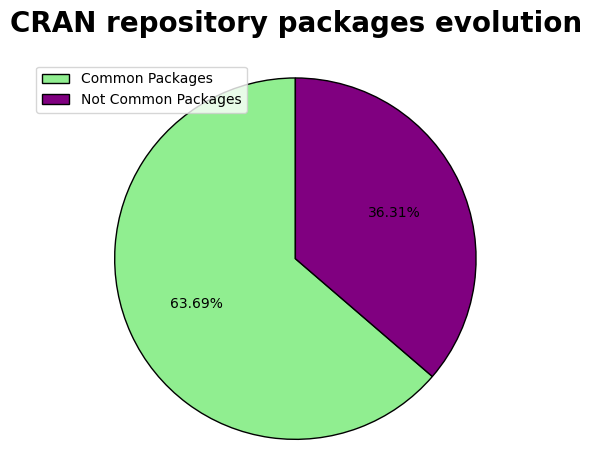
\includegraphics[width=0.7\textwidth]{img/cran/circle.png}
        \caption{Comparación de los paquetes comunes entre los dos conjuntos de datos.}
        \label{fig:cran_common_packages2}
    \end{center}
\end{figure}

\begin{figure}[ht!]
    \begin{center}
        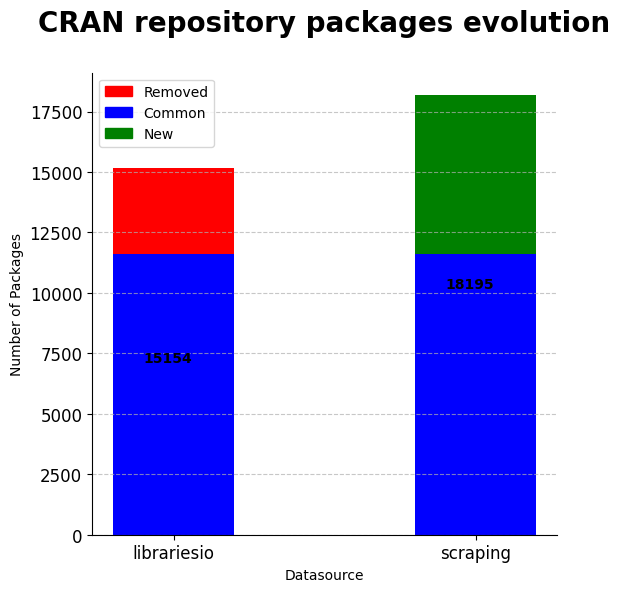
\includegraphics[width=0.6\textwidth]{img/cran/bars.png}
        \caption{Comparación del número de paquetes.}
        \label{fig:cran_common_packages3}
    \end{center}
\end{figure}

Por consiguiente, se concluye que el conjunto de datos \textit{Scraped} proporciona una
visión más completa y actualizada de los paquetes disponibles. Al incluir tanto los paquetes
en común como los paquetes adicionales respecto a \textit{Libraries.io}, \textit{Scraped}
se configura como una fuente valiosa para investigaciones y análisis en el ámbito de estudio.


\subsection{El tamaño}

A continuación realizaremos una comparación de las medidas de tamaño entre los dos conjuntos de datos y como es
el agrupamiento de los nodos en cada uno de ellos. \ref{tab:cran_size}

\begin{table}[ht!]
    \begin{center}
        \begin{tabular}{|l|c|c|c|}
            \hline
            \textbf{Medida}                & \textbf{Libraries.io} & \textbf{Scraped} \\
            \hline
            Number of nodes                & 15647                 & 18671            \\
            Number of edges                & 76207                 & 113273           \\
            Average degree                 & 9.740                 & 12.133           \\
            Average clustering coefficient & 0.131                 & 0.152            \\
            \hline
        \end{tabular}
        \caption{Comparación de medidas de tamaño entre los dos conjuntos de datos.}
        \label{tab:cran_size}
    \end{center}
\end{table}

La red \textit{Scraped} tiene un mayor número de nodos (\textit{18671}) en comparación con la
red \textit{Libraries.io} (\textit{15647}). Esto indica que \textit{Scraped} contiene más elementos o entidades
interconectadas en su estructura de red.

La red \textit{Scraped} también tiene un mayor número de aristas o enlaces (\textit{113273}) en
comparación con la red \textit{Libraries.io} (\textit{76207}). Esto implica que \textit{Scraped} tiene más
conexiones entre los nodos, lo que aumenta su grado de conectividad.

El grado promedio de los nodos en la red \textit{Scraped} es más alto (\textit{12.133}) en
comparación con el de la red \textit{Libraries.io} (\textit{9.740}). Esto sugiere que, en promedio, cada nodo
en \textit{Scraped} tiene más conexiones con otros nodos en comparación con los nodos en \textit{Libraries.io}.

El coeficiente de agrupamiento promedio en la red \textit{Scraped} es
ligeramente más alto (\textit{0.152}) que en la red \textit{Libraries.io} (\textit{0.131}). Esto indica que,
en promedio, los nodos en \textit{Scraped} tienen una mayor tendencia a formar grupos o comunidades más densamente
interconectadas en comparación con los nodos en \textit{Libraries.io}.

\subsection{El grado}

\begin{figure}[ht!]
    \begin{center}
        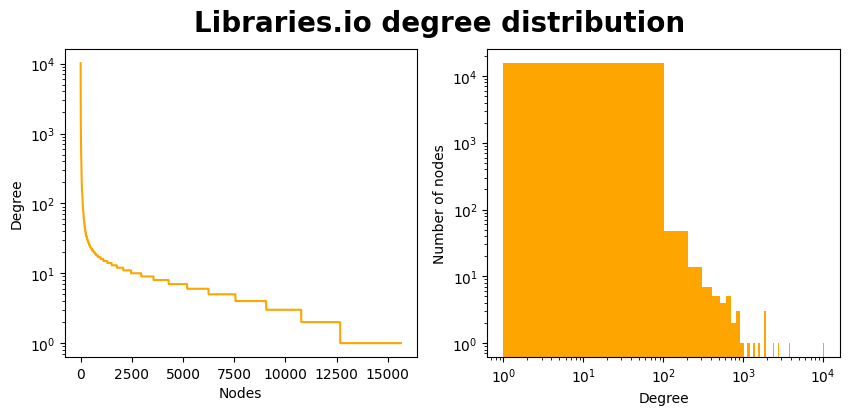
\includegraphics[width=1\textwidth]{img/cran/distribucion_grado.png}
        \caption{Distribución de grado \textit{Libraries.io}.}
        \label{fig:cran_degree_distribution}
    \end{center}
\end{figure}

\begin{figure}[ht!]
    \begin{center}
        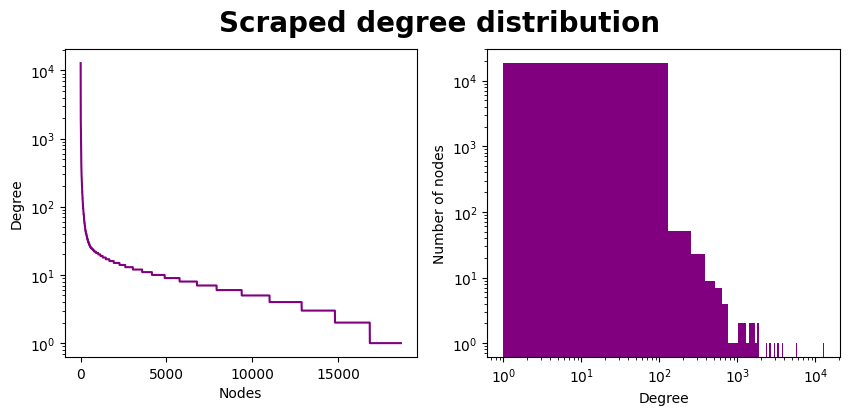
\includegraphics[width=1\textwidth]{img/cran/distribucion_grado2.png}
        \caption{Distribución de grado \textit{Scraped}.}
        \label{fig:cran_degree_distribution_scraped}
    \end{center}
\end{figure}

Al realizar una comparativa de las distribuciones de grado entre ambos conjuntos de datos,
se evidencia un leve incremento en el grado promedio. El grado promedio del conjunto de datos
\textit{Libraries.io} es de 4.87, mientras que en el conjunto \textit{Scraped} alcanza un valor
de 6.06. Estos resultados indican un incremento en la conectividad y la relevancia de los
paquetes más destacados en el conjunto de datos \textit{Scraped}. Tal variación en los valores
promedio refleja el aumento en la importancia y la interconexión de los paquetes dentro de este
conjunto de datos, lo cual puede estar relacionado con su mayor tamaño y actualización.
\ref{fig:cran_degree_distribution} \ref{fig:cran_degree_distribution_scraped}

Además, se observa que la tendencia a disminuir el número de dependencias es ligeramente
más pronunciada que la tendencia a aumentarlas. Esto sugiere que, en la evolución de
la red de dependencias, los paquetes tienden a reducir su dependencia directa o a
reorganizar sus conexiones con otros paquetes, lo que puede ser resultado de procesos
de \textit{refactorización}, \textit{optimización} o \textit{consolidación}.


\subsubsection{Grado de salida (\textit{out degree})}


En el análisis de la distribución del grado de salida, no se observan diferencias significativas
que puedan ser comparadas. Podemos inferir que ambas distribuciones siguen una tendencia
similar, con la única distinción de que en el conjunto de datos nuevo se encuentra un mayor
número de nodos \ref{fig:cran_out_lib} \ref{fig:cran_out_scraped}.

\begin{figure}[ht!]
    \begin{center}
        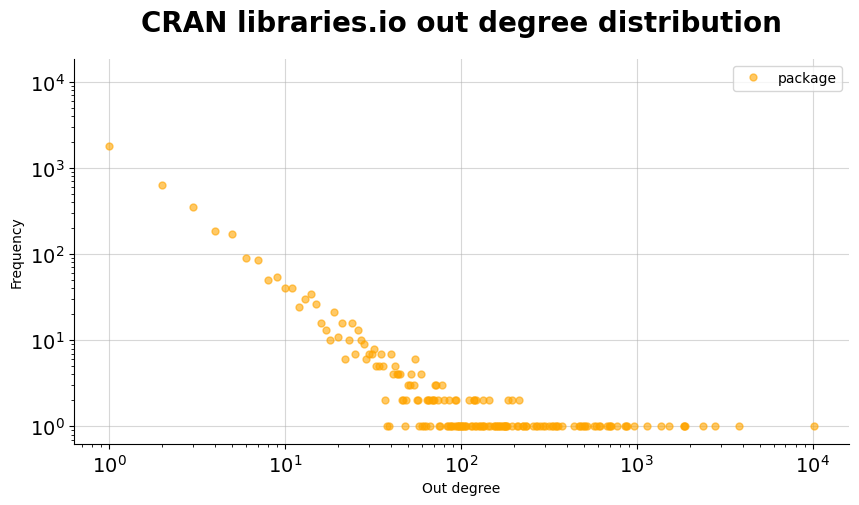
\includegraphics[width=1\textwidth]{img/cran/out_deg.png}
        \caption{Distribución de Out degree de \textit{Libraries.io}.}
        \label{fig:cran_out_lib}
    \end{center}
\end{figure}

\begin{figure}[ht!]
    \begin{center}
        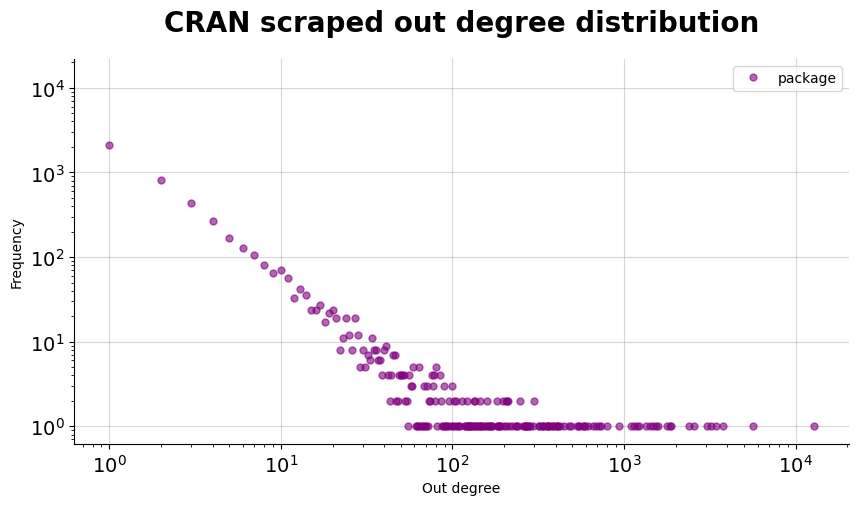
\includegraphics[width=1\textwidth]{img/cran/out_deg2.png}
        \caption{Distribución de Out degree de \textit{Scraped}.}
        \label{fig:cran_out_scraped}
    \end{center}
\end{figure}

Al examinar el conjunto de paquetes con mayor grado de salida, se observa un aumento generalizado
en todos ellos. Estos paquetes destacados representan una centralidad de grado significativa,
lo que implica que son las dependencias más utilizadas dentro del sistema. Es comprensible que
estos paquetes, al ser ampliamente utilizados, hayan mantenido una presencia constante en la
red y hayan experimentado un incremento en el número de sus dependientes debido al surgimiento
de nuevos paquetes. \ref{fig:cran_out_libio_top}

\begin{figure}[ht!]
    \begin{center}
        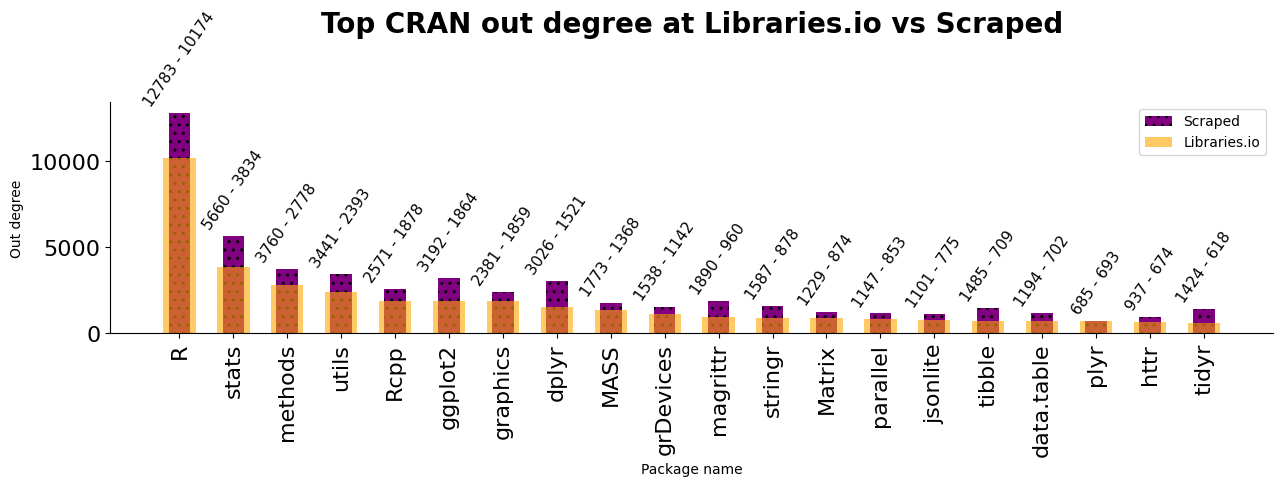
\includegraphics[width=1\textwidth]{img/cran/out_lib.png}
        \caption{Top paquetes con mayor grado de salida en \textit{Libraries.io}.}
        \label{fig:cran_out_libio_top}
    \end{center}
\end{figure}

Esta observación refuerza la importancia y la relevancia de estos paquetes clave en el
ecosistema estudiado. Su estabilidad y el aumento en sus dependientes pueden atribuirse a
su funcionalidad y a su amplia adopción por parte de los usuarios. Además, el incremento en
la cantidad de dependientes es un indicativo del crecimiento y la evolución continua del
sistema, donde se generan nuevas relaciones de dependencia entre los paquetes existentes
y los recién agregados.

Al realizar la comparativa utilizando el nuevo conjunto de datos, se observa que los principales
representantes del ranking se mantienen presentes. Sin embargo, se han producido algunas variaciones
en el orden de algunos puestos dentro del top. Además, se ha registrado la inclusión de paquetes que
previamente se encontraban fuera del top. \ref{fig:cran_out_scraped_top}

\begin{figure}[ht!]
    \begin{center}
        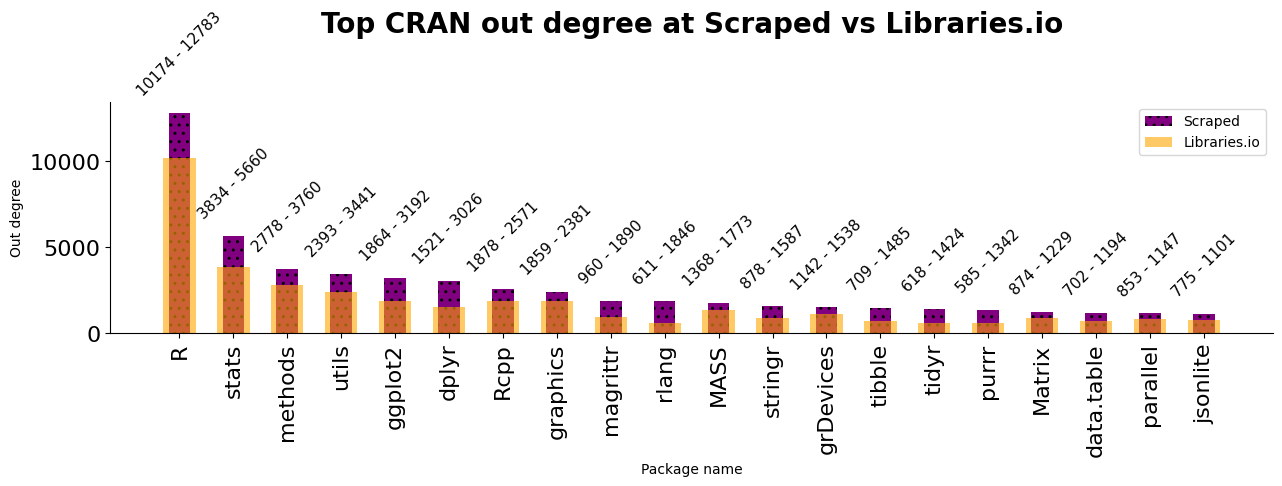
\includegraphics[width=1\textwidth]{img/cran/out_scr.png}
        \caption{Top paquetes con mayor grado de salida en \textit{Scraped}.}
        \label{fig:cran_out_scraped_top}
    \end{center}
\end{figure}

Esta inclusión de paquetes puede atribuirse al incremento en el número de sus dependencias,
el cual ha superado a aquellos que han salido del top en este periodo de tiempo analizado.
Estos nuevos paquetes han logrado adquirir una mayor relevancia y han fortalecido su posición
dentro del conjunto de datos. Este fenómeno puede ser consecuencia de su creciente adopción y
de la expansión de su funcionalidad, lo que ha llevado a un incremento en el número de paquetes
que los utilizan como dependencias.

Este incremento lo podemos ver representado en la siguiente figura \ref{fig:cran_dependents_dist}.

\begin{figure}[ht!]
    \begin{center}
        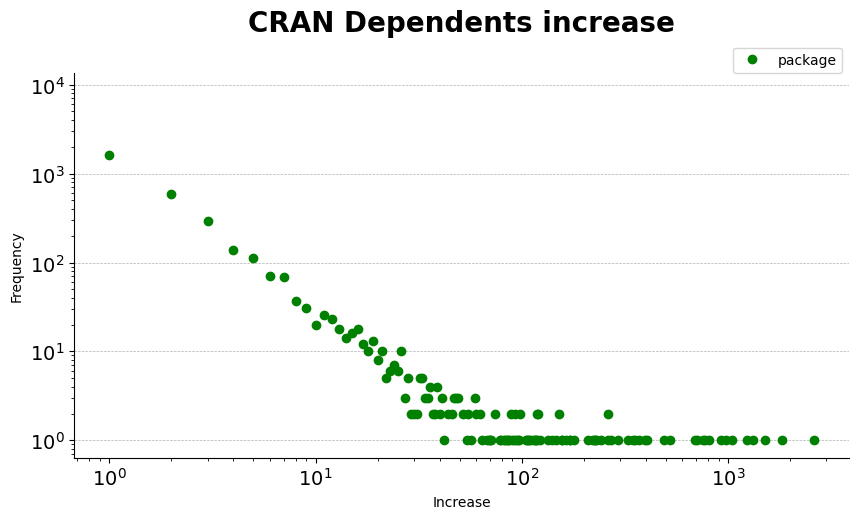
\includegraphics[width=1\textwidth]{img/cran/dependents_dist.png}
        \caption{Distribución de dependientes.}
        \label{fig:cran_dependents_dist}
    \end{center}
\end{figure}

\subsubsection{Grado de entrada (\textit{in degree})}


En el análisis de la distribución del grado de entrada, se observa un comportamiento común
en ambos conjuntos de datos. Debido a su similitud, resulta difícil extraer conclusiones
significativas. Sin embargo, se puede observar un ligero incremento en el nuevo conjunto de
datos en comparación con el conjunto de datos de Libraries.io. \ref{fig:cran_in_lib} \ref{fig:cran_in_scraped}

\begin{figure}[ht!]
    \begin{center}
        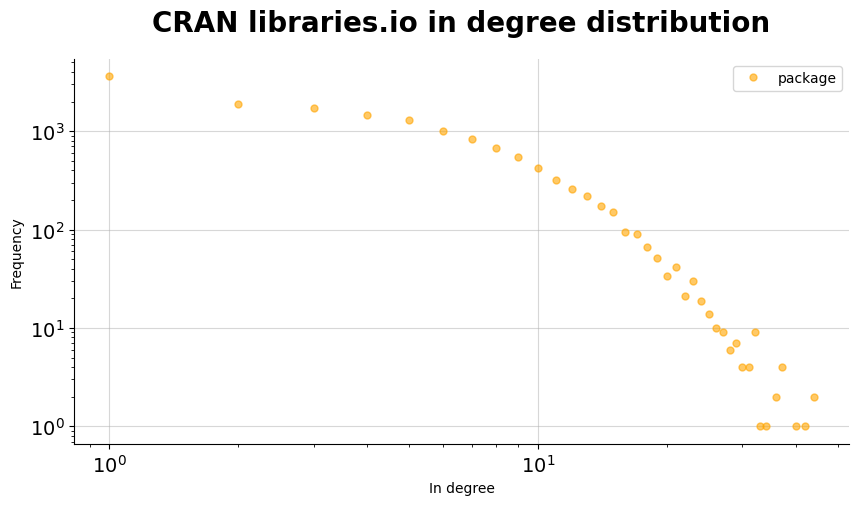
\includegraphics[width=0.8\textwidth]{img/cran/ind_lib.png}
        \caption{Distribución de In degree de \textit{Libraries.io}.}
        \label{fig:cran_in_lib}
    \end{center}
\end{figure}

\begin{figure}[ht!]
    \begin{center}
        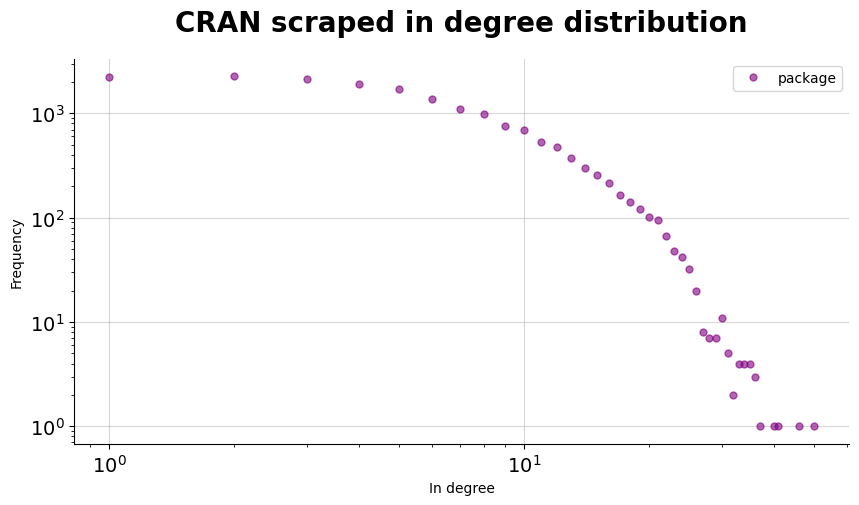
\includegraphics[width=0.8\textwidth]{img/cran/ind_scr.png}
        \caption{Distribución de In degree de \textit{Scraped}.}
        \label{fig:cran_in_scraped}
    \end{center}
\end{figure}

Tomando como punto de referencia la frecuencia de nodos con un grado de entrada de valor 20,
en el conjunto de datos de Libraries.io se encuentran alrededor de 50 nodos, mientras que en
el nuevo conjunto de datos se registran aproximadamente 100 nodos. Estos valores pueden sugerir
un aumento en la cantidad de paquetes que reciben un número determinado de dependencias.


Si representamos el \textit{top} de \textit{in degree} de los paquetes del conjunto de datos
de \textit{Libraries.io}, podemos identificar aquellos paquetes que poseen un mayor número de
dependencias. Estos paquetes podrían considerarse los más vulnerables en su primer nivel de dependencia,
sin tener en cuenta la transitividad. Al analizar los resultados, se puede concluir que un porcentaje
significativo de los paquetes destacados en este \textit{top} han mantenido su presencia en la red a
lo largo del tiempo.

Además, se observa una tendencia general a disminuir el número de dependencias para la mayoría de
los casos en el \textit{top}. Esto sugiere que, a medida que evoluciona la red de dependencias,
algunos paquetes han logrado reducir su dependencia directa o han redistribuido sus conexiones
con otros paquetes.


\begin{figure}[ht!]
    \begin{center}
        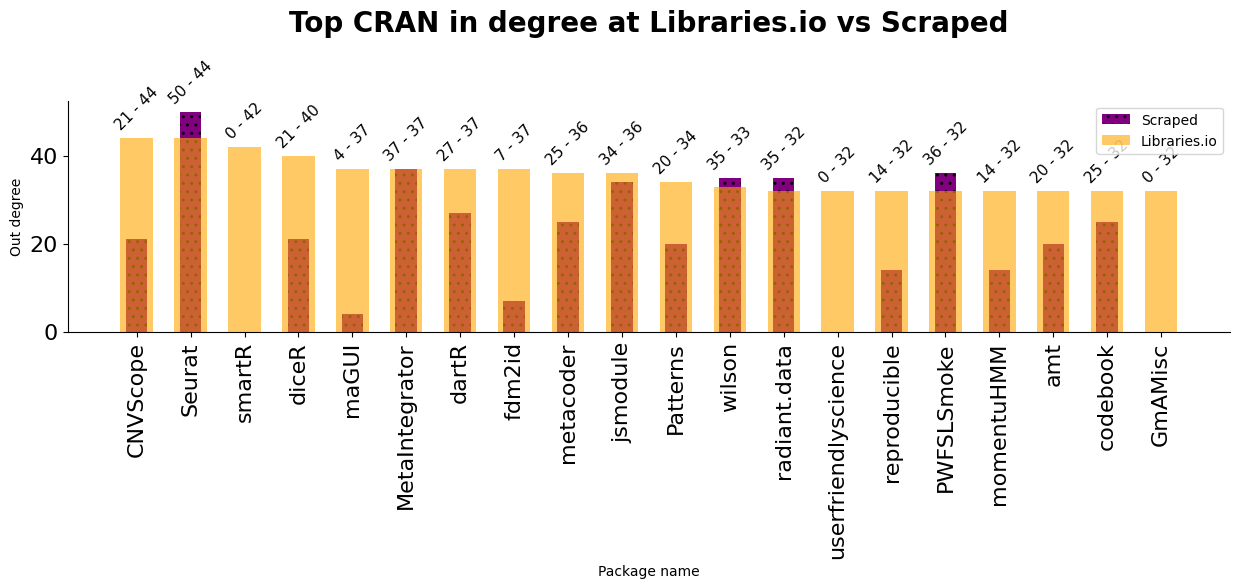
\includegraphics[width=1\textwidth]{img/cran/top_ind_libio.png}
        \caption{Top paquetes con mayor grado de entrada en \textit{Libraries.io}.}
        \label{fig:top_ind_libio_cran}
    \end{center}
\end{figure}


Desde la perspectiva del \textit{top} de \textit{in degree}, se observa una notable variación en
la evolución de los paquetes. Aproximadamente la mitad de los individuos que conformaban el
\textit{top} han sido reemplazados. Estos paquetes de reemplazo se caracterizan por ser nuevos
en la red, lo cual sugiere que están utilizando funcionalidades previamente desarrolladas para
generar nuevas capacidades.

Es común que aparezcan nuevos paquetes en este \textit{top}, dado el contexto de una red de
carácter científico. A medida que el software madura, es habitual que estos paquetes más
jóvenes se refactoricen con el tiempo, tendiendo a disminuir sus dependencias.

Por otro lado, existen paquetes que no sólo se encontraban en el \textit{top} anterior,
sino que han incrementado sus dependencias. Este aumento puede ser indicativo de paquetes
cuya funcionalidad aún está en desarrollo y continúa evolucionando. \ref{fig:top_ind_scraped_cran}

\begin{figure}[ht!]
    \begin{center}
        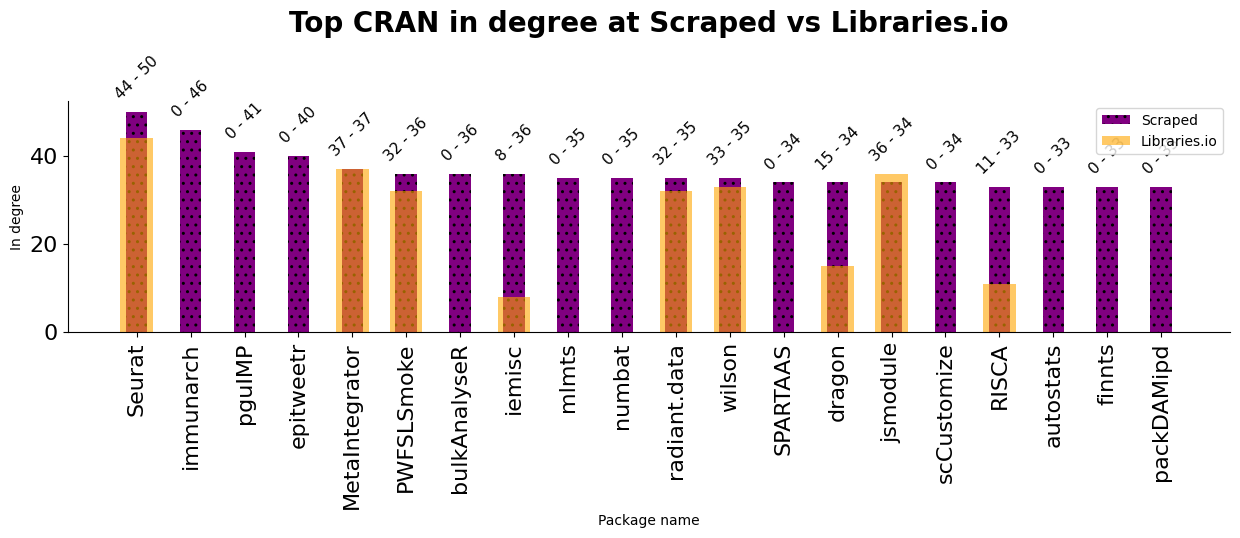
\includegraphics[width=1\textwidth]{img/cran/top_ind_scraped.png}
        \caption{Top paquetes con mayor grado de entrada en \textit{Scraped}.}
        \label{fig:top_ind_scraped_cran}
    \end{center}
\end{figure}


Al observar la tendencia del incremento de dependencias en la red, se evidencia que, en
general, es común que el número de dependencias de los paquetes no experimente cambios
drásticos. La mayoría de los paquetes se sitúan en un rango de incremento de dependencias
de aproximadamente $\pm$10. \ref{fig:cran_dependencies_increase}


\begin{figure}[ht!]
    \begin{center}
        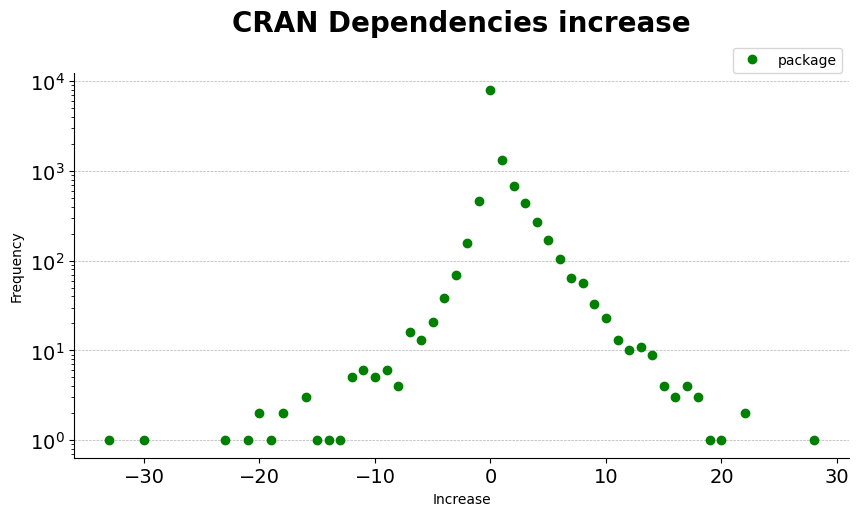
\includegraphics[width=1\textwidth]{img/cran/dependencies_increase.png}
        \caption{Incremento de dependencias.}
        \label{fig:cran_dependencies_increase}
    \end{center}
\end{figure}

\subsection{El \textit{PageRank}}

A partir del análisis de la distribución de \textit{PageRank} en la red, se observa la presencia
de numerosos nodos con un \textit{PageRank} bajo, y a medida que se incrementa el valor del
\textit{PageRank}, la frecuencia de nodos disminuye gradualmente. Este patrón revela la
existencia de muchos nodos de baja importancia en la red, junto con un grupo reducido de
paquetes que son considerados importantes debido a sus dependencias, las cuales, a su vez,
son también dependencias relevantes en la red.

Al comparar las dos distribuciones, se aprecia una diferencia notable en la red
de \textit{Libraries.io}, donde el valor máximo alcanzado por el \textit{PageRank} de
un paquete es mayor en comparación con la nueva red. Esta diferencia puede interpretarse
como un indicio de que, en la evolución de \textit{CRAN}, los paquetes más importantes
se han estabilizado, mientras que han surgido otros paquetes que están adquiriendo
relevancia. Como resultado, el \textit{PageRank} se ha distribuido de manera más equitativa
entre los paquetes de la red. \ref{fig:cran_pr_libio} \ref{fig:cran_pr_scraped}

\begin{figure}[ht!]
    \begin{center}
        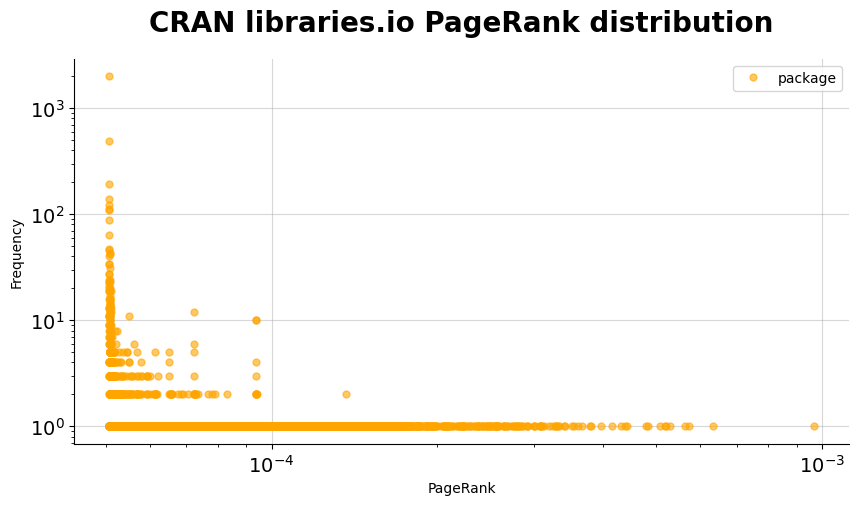
\includegraphics[width=1\textwidth]{img/cran/pr.png}
        \caption{Distribución de \textit{PageRank} en \textit{Libraries.io}.}
        \label{fig:cran_pr_libio}
    \end{center}
\end{figure}

\begin{figure}[ht!]
    \begin{center}
        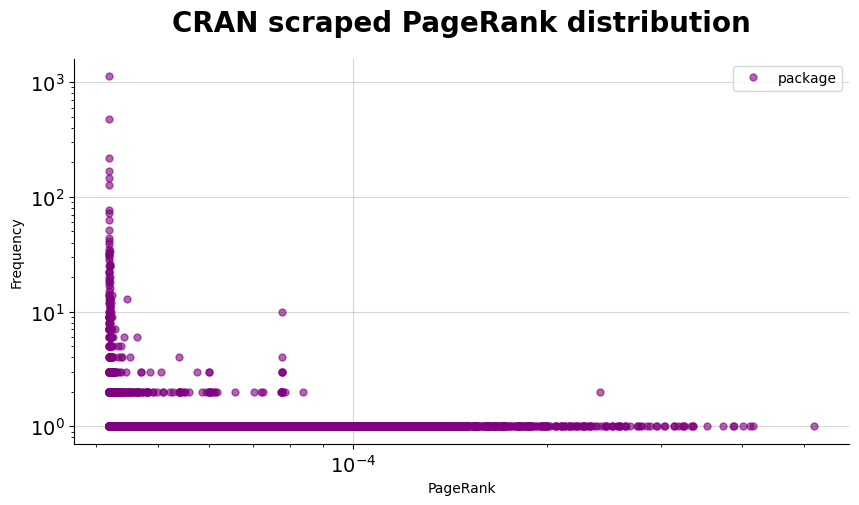
\includegraphics[width=1\textwidth]{img/cran/pr2.png}
        \caption{Distribución de \textit{PageRank} en \textit{Scraped}.}
        \label{fig:cran_pr_scraped}
    \end{center}
\end{figure}

El top de mayor \textit{PageRank} en \textit{Libraries.io} nos brinda una visión de los paquetes que se
consideran como nodos vulnerables en la red de dependencias. Esto implica que son elementos no fundamentales
para la funcionalidad y el rendimiento de otros paquetes, y que poseen un mayor número de dependencias
directas e indirectas.

Estos paquetes tienden a ser dependientes de otros paquetes con alto \textit{PageRank}. Además, desde el
punto de vista de la vulnerabilidad, son considerados críticos debido a que suelen acumular una alta
dependencia transitiva. Esto significa que cualquier cambio o problema en sus dependencias transitivas puede
tener un impacto en el.

Estos nodos de alto \textit{PageRank} juegan un papel crucial en el mantenimiento y la estabilidad de la
red de dependencias. Su importancia radica en que son candidatos a desaparecer. \ref{fig:cran_pr_libio_top}

\begin{figure}[ht!]
    \begin{center}
        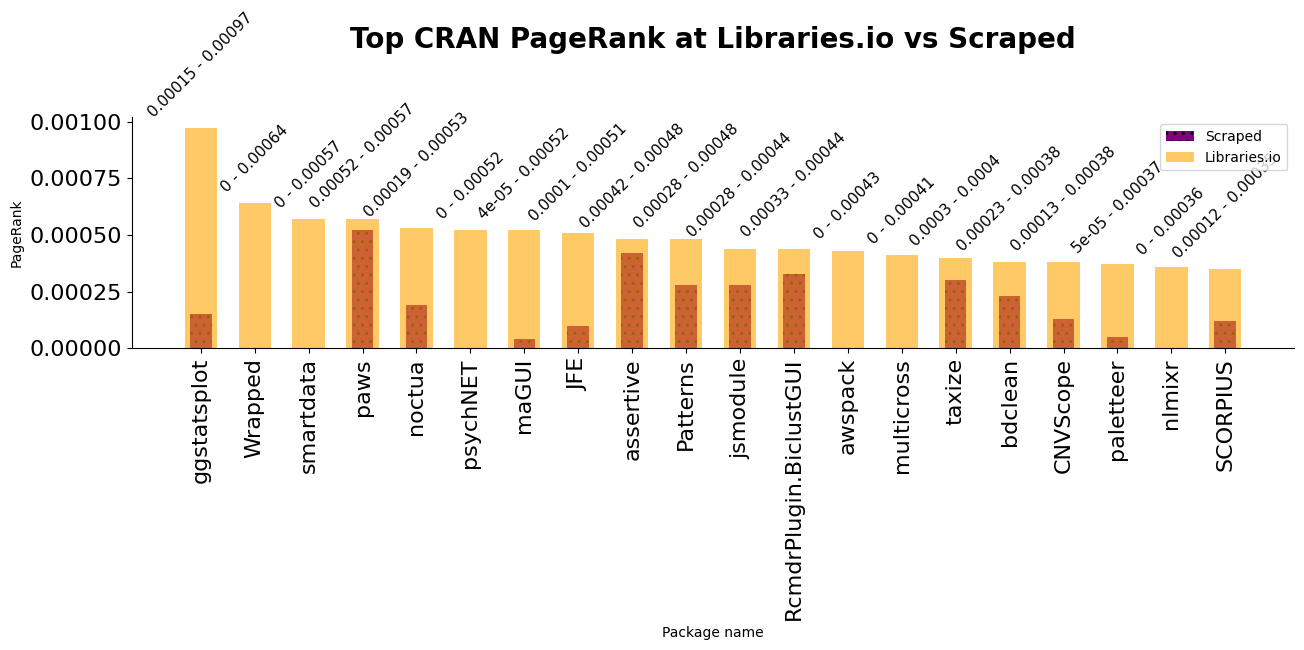
\includegraphics[width=1\textwidth]{img/cran/pr_top.png}
        \caption{Top \textit{PageRank} en \textit{Libraries.io}.}
        \label{fig:cran_pr_libio_top}
    \end{center}
\end{figure}


En base a la introducción anterior, es esperable encontrar paquetes en el top de \textit{Libraries.io}
que no estén presentes en el conjunto de datos de \textit{Scraped}.

\begin{figure}[ht!]
    \begin{center}
        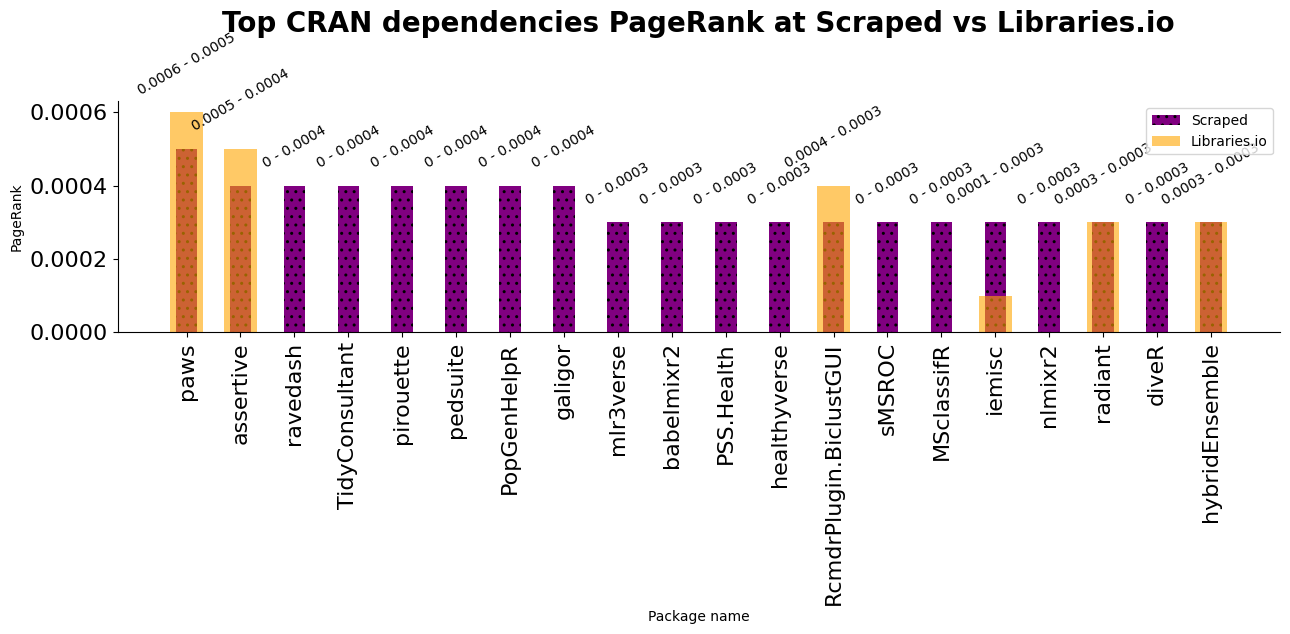
\includegraphics[width=1\textwidth]{img/cran/pr_top2.png}
        \caption{Top \textit{PageRank} en \textit{Scraped}.}
        \label{fig:cran_pr_scraped_top}
    \end{center}
\end{figure}

A partir del nuevo conjunto de datos \ref{fig:cran_pr_scraped_top}, se observa un descenso general en los
valores de PageRank en comparación con el conjunto de datos de \textit{Libraries.io}. Además, se destaca
que un gran número de paquetes han ingresado al top de PageRank y no estaban presentes en \textit{Libraries.io}.
Este hallazgo refuerza la teoría de que el PageRank, en el contexto de una red de dependencias, puede
considerarse un indicador de la vulnerabilidad de un paquete. Se puede inferir que estos paquetes recién
incorporados tienden a tener una presencia transitoria en la red y, debido a su relativa falta de madurez,
es probable que experimenten variaciones significativas a lo largo del tiempo.

Sin embargo, resulta más interesante centrar la atención en aquellos paquetes que mantienen un alto valor de
PageRank a lo largo del tiempo. Estos paquetes indican la presencia de dependencias con alto PageRank y altamente
transitivas en la red, lo que los hace potencialmente más vulnerables. Su capacidad para conservar su
importancia en el contexto de la evolución de la red sugiere que desempeñan un papel fundamental en el
funcionamiento y la estabilidad de otros paquetes. \ref{fig:Top 20 PageRank número de dependencias transitivas en Libraries.io}
\ref{fig:Top 20 PageRank número de dependencias transitivas en Scraped}

\begin{figure}[ht!]
    \begin{center}
        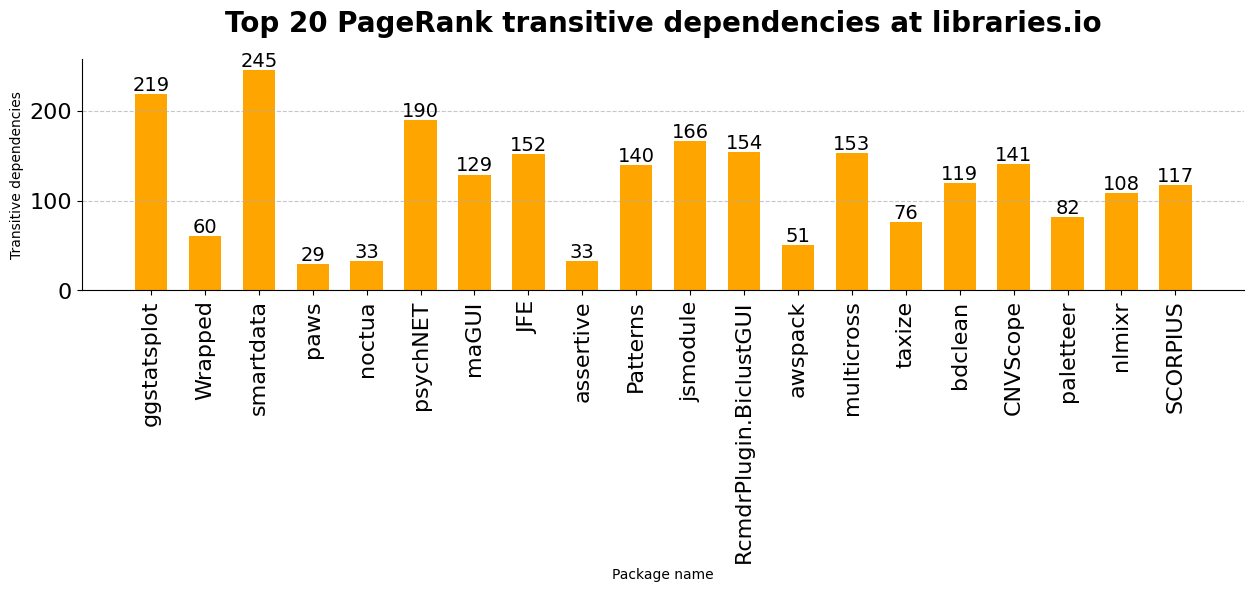
\includegraphics[width=1\textwidth]{img/cran/pr_trans.png}
        \caption{Top 20 \textit{PageRank} número de dependencias transitivas en Libraries.io}
        \label{fig:Top 20 PageRank número de dependencias transitivas en Libraries.io}
    \end{center}
\end{figure}

\begin{figure}[ht!]
    \begin{center}
        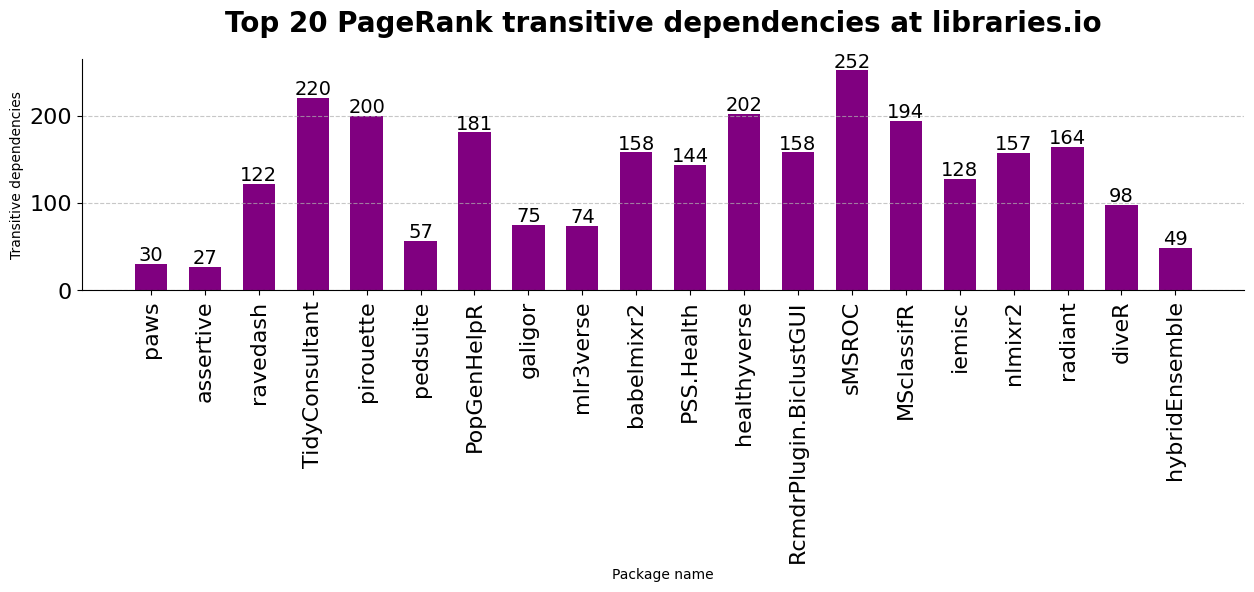
\includegraphics[width=1\textwidth]{img/cran/pr_trans2.png}dependidos
        \caption{Top 20 \textit{PageRank} número de dependencias transitivas en Scraped}
        \label{fig:Top 20 PageRank número de dependencias transitivas en Scraped}
    \end{center}
\end{figure}

Desde una perspectiva inversa, el uso del \textit{PageRank} nos permite identificar qué paquetes son las dependencias
más importantes en la red de dependencias. Esto proporciona una visión de
la centralidad en términos de popularidad de un paquete. Al analizar el \textit{PageRank} bajo esta perspectiva, es
posible determinar qué paquetes son altamente requeridos por otros paquetes y, por lo tanto,
desempeñan un papel crucial en el funcionamiento de la red. \ref{fig:Top 20 PageRank paquetes en Scraped}
Estos paquetes tienen que ser mimados y cuidados, ya que cualquier cambio en ellos puede tener un impacto
en la red de dependencias. Por suerte son poco vulnerables, ya que no dependen de otros paquetes.

\begin{figure}[ht!]
    \begin{center}
        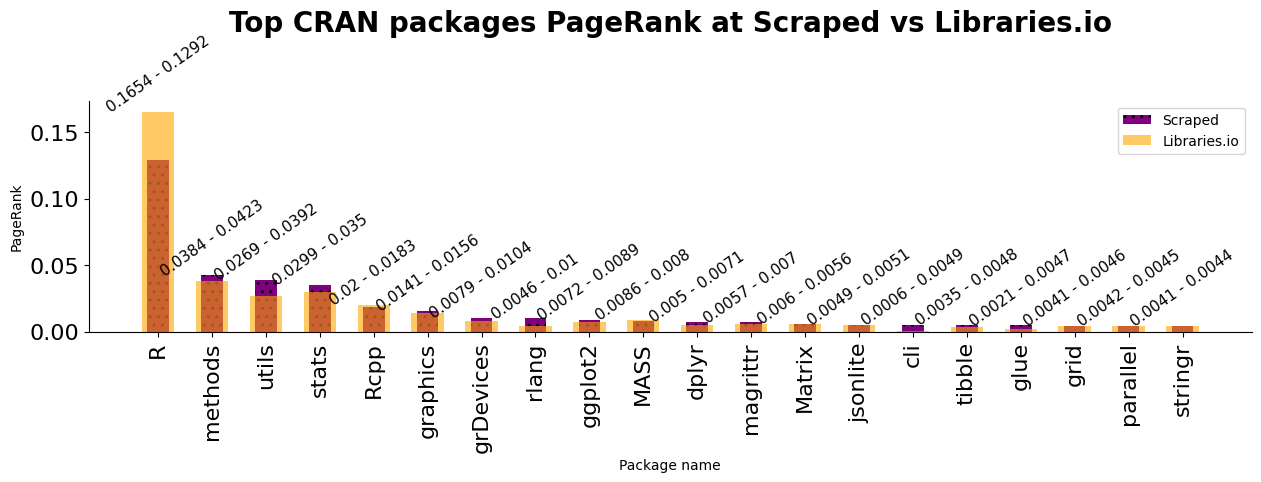
\includegraphics[width=1\textwidth]{img/cran/pr_inverted.png}
        \caption{Top 20 \textit{PageRank} paquetes en Scraped}
        \label{fig:Top 20 PageRank paquetes en Scraped}
    \end{center}
\end{figure}

Los paquetes mostrados en este top son los más populares del ecosistema de \textit{R}.
Estos paquetes son los más utilizados por otros paquetes, lo que los hace fundamentales para el
funcionamiento de la red de dependencias. No es raro que el paquete R, que implementa el \textit{core}
del lenguaje, sea el paquete más popular.

\begin{figure}[ht!]
    \begin{center}
        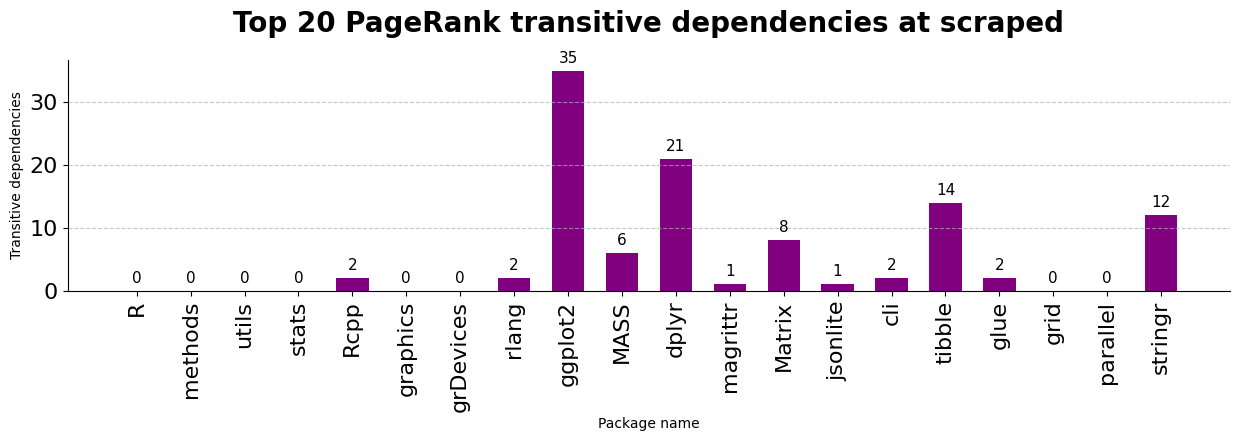
\includegraphics[width=1\textwidth]{img/cran/transitive_pr_scr.png}
        \caption{Top 20 \textit{PageRank} paquetes número de dependencias transitivas en Scraped}
        \label{fig:Top 20 PageRank paquetes número de dependencias transitivas en Scraped}
    \end{center}
\end{figure}

Estos paquetes a nivel de vulnerabilidad son los más estables, ya que el número de dependencias
transitivas que tienen es relativamente bajo. \ref{fig:Top 20 PageRank paquetes número de dependencias transitivas en Scraped}

\subsection{Impacto (\textit{Impact})}

Desde el punto de vista de esta metrica, podemos interpretar la vulnerabilidad de un paquete como el número
de dependencias paquetes que se ven afectados por un cambio en el paquete. En este sentido, un paquete
vulnerable es aquel que tiene un alto impacto en la red de dependencias.

\begin{figure}[ht!]
    \begin{center}
        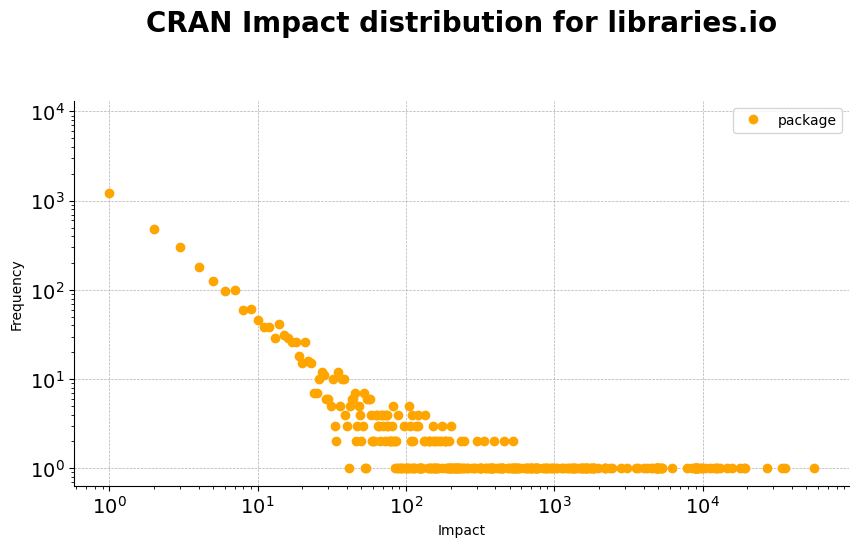
\includegraphics[width=0.8\textwidth]{img/cran/impact_dist_libio.png}
        \caption{Distribución de \textit{Impact} en Libraries.io}
        \label{fig:Distribución de Impact en Libraries.io}
    \end{center}
\end{figure}

\begin{figure}[ht!]
    \begin{center}
        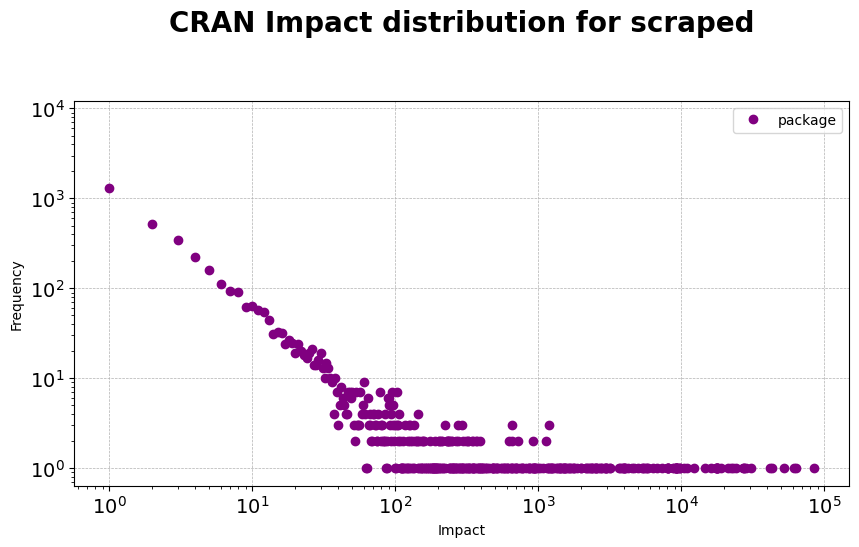
\includegraphics[width=0.8\textwidth]{img/cran/impact_dist_scraped.png}
        \caption{Distribución de \textit{Impact} en Scraped}
        \label{fig:Distribución de Impact en Scraped}
    \end{center}
\end{figure}

A partir del análisis de la distribución del impacto, se observa una tendencia similar en ambos
conjuntos de datos. Se aprecia un ligero incremento en el impacto en el nuevo conjunto de datos,
pero en general los valores se mantienen estables. Este incremento puede atribuirse a la incorporación
de nuevos paquetes en la red, los cuales han adoptado dependencias existentes, lo que ha aumentado el
impacto de estas últimas. \ref{fig:Distribución de Impact en Libraries.io} \ref{fig:Distribución de Impact en Scraped}


En el top de paquetes con mayor \textit{impacto} se encuentran aquellos que son considerados los más populares
en la red, en términos de su influencia sobre otros paquetes. Es notable que los principales representantes
de este top también aparecen en el top del \textit{PageRank} a nivel de la red de paquetes. Desde el punto
de vista de la \textit{dependencia transitiva}, estos paquetes son aquellos que tienen la mayor cantidad de
dependientes en toda la red.

Al analizar el \textit{impacto} de estos paquetes, se observa un aumento en su valor, en algunos casos
significativo. Esto indica que estos paquetes han demostrado ser estables en el tiempo y en su implementación,
y que su funcionalidad es altamente útil para la red.

\begin{figure}[ht!]
    \begin{center}
        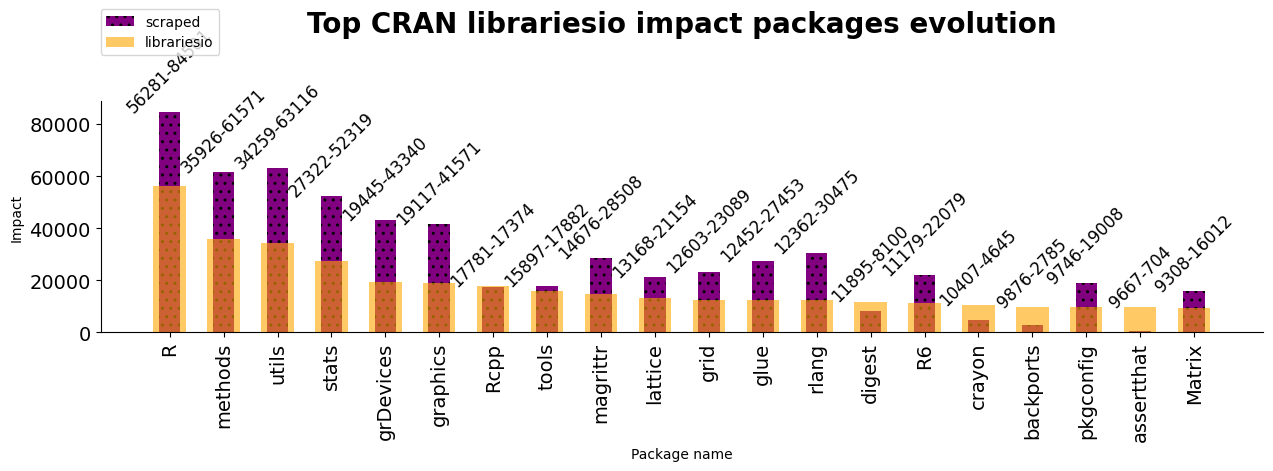
\includegraphics[width=1\textwidth]{img/cran/impact_top_libio.png}
        \caption{Top paquetes con mayor \textit{Impact} en Libraries.io}
        \label{fig:Top impact Libraries.io}
    \end{center}
\end{figure}

\begin{figure}[ht!]
    \begin{center}
        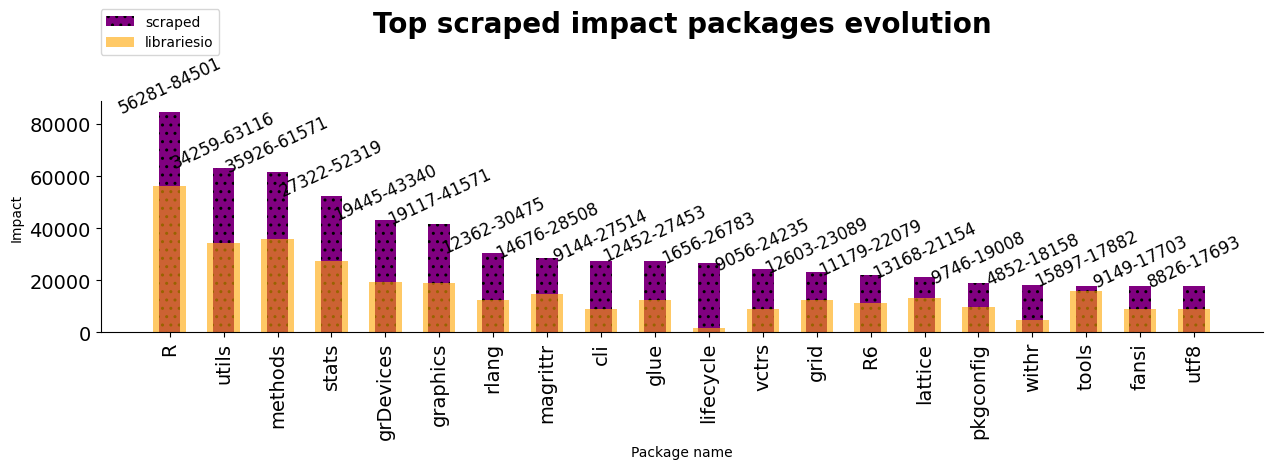
\includegraphics[width=1\textwidth]{img/cran/impact_top_scraped.png}
        \caption{Top paquetes con mayor \textit{Impact} en Scraped}
        \label{fig:Top impact Scraped}
    \end{center}
\end{figure}

Por otro lado, aquellos paquetes en el top que han experimentado una reducción en su \textit{impacto}
podrían indicar la aparición de otros paquetes con funcionalidades similares o mejoradas, los cuales han
sido elegidos como alternativas por los usuarios de la red. \ref{fig:Top impact Libraries.io} \ref{fig:Top impact Scraped}

\begin{table}[ht!]
    \begin{center}
        \begin{tabular}{|l|r|r|r|}
            \hline
            \textbf{Package} & \textbf{Libraries.io} & \textbf{Scraped} & \textbf{increment} \\
            \hline
            utils            & 34259                 & 63116            & 28857              \\
            R                & 56281                 & 84501            & 28220              \\
            methods          & 35926                 & 61571            & 25645              \\
            lifecycle        & 1656                  & 26783            & 25127              \\
            stats            & 27322                 & 52319            & 24997              \\
            grDevices        & 19445                 & 43340            & 23895              \\
            graphics         & 19117                 & 41571            & 22454              \\
            cli              & 9144                  & 27514            & 18370              \\
            rlang            & 12362                 & 30475            & 18113              \\
            vctrs            & 9056                  & 24235            & 15179              \\
            \hline
        \end{tabular}
        \caption{Top 10 paquetes con mayor incremento en \textit{Impact}}
        \label{tab:Top 10 paquetes con mayor incremento en Impact}
    \end{center}
\end{table}

\begin{table}[ht!]
    \begin{center}
        \begin{tabular}{|l|r|r|r|}
            \hline
            \textbf{Package} & \textbf{Libraries.io} & \textbf{Scraped} & \textbf{increment} \\
            \hline
            zeallot          & 9070                  & 67               & -9003              \\
            assertthat       & 9667                  & 704              & -8963              \\
            backports        & 9876                  & 2785             & -7091              \\
            crayon           & 10407                 & 4645             & -5762              \\
            reshape2         & 5217                  & 1232             & -3985              \\
            digest           & 11895                 & 8100             & -3795              \\
            plyr             & 6265                  & 2710             & -3555              \\
            lazyeval         & 4662                  & 1193             & -3469              \\
            formatR          & 1450                  & 90               & -1360              \\
            markdown         & 1511                  & 324              & -1187              \\
            \hline
        \end{tabular}
    \end{center}
    \caption{Top 10 paquetes con mayor decremento en \textit{Impact}}
    \label{tab:Top 10 paquetes con mayor decremento en Impact}
\end{table}


En la tablas del incremento podemos ver que los paquetes que han tenido un mayor incremento y decremento
en su impacto. \ref{tab:Top 10 paquetes con mayor incremento en Impact} \ref{tab:Top 10 paquetes con mayor decremento en Impact}



\begin{figure}[ht!]
    \begin{center}
        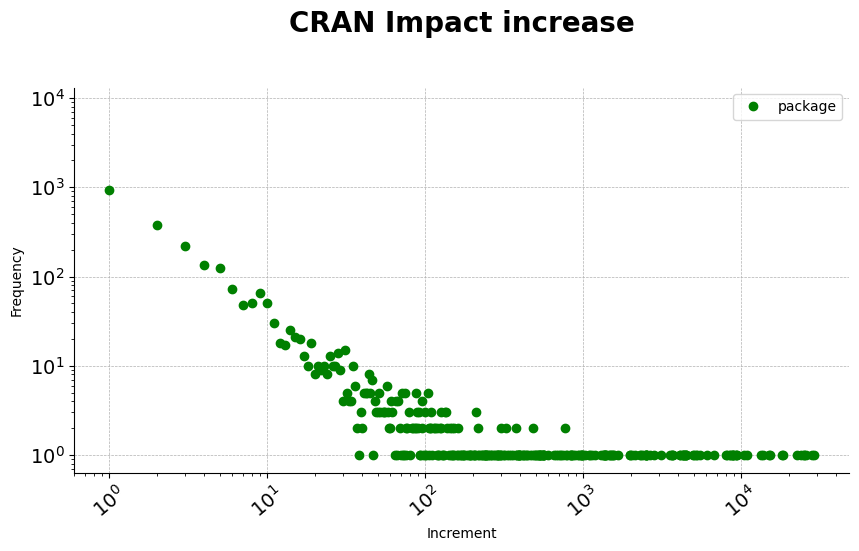
\includegraphics[width=1\textwidth]{img/cran/impact_increase_dist.png}
        \caption{Incremento de \textit{Impact}}
        \label{fig:Incremento de Impact}
    \end{center}
\end{figure}

Si lo representamos gráficamente se obtiene una tendencia similar a las distribuciones anteriores. \ref{fig:Incremento de Impact}

\subsection{Alcance (\textit{Reach})}

El alcance (\textit{Reach}) de un paquete p, equivale al número de sucesores transitivos
de p más 1 y mide el número de paquetes potencialmente afectados
por un defecto en p.

A la vista de las siguientes tablas podemos observar que  paquetes
son los que tienen un mayor reach. \ref{tab:Top 10 paquetes con mayor Reach}

\begin{table}[ht!]
    \begin{center}
        \begin{tabular}{|c|c|}
            \hline
            \textbf{Libraries.io} & \textbf{Scraped} \\
            \hline
            R, 14395              & R, 17223         \\
            methods, 10839        & methods, 15103   \\
            utils, 10516          & utils, 15037     \\
            stats, 9850           & stats, 14360     \\
            graphics, 7938        & graphics, 12809  \\
            grDevices, 7382       & grDevices, 12763 \\
            Rcpp, 7380            & grid, 9241       \\
            lattice, 6296         & rlang, 8993      \\
            tools, 6127           & lattice, 8945    \\
            grid, 5971            & magrittr, 8916   \\
            \hline
        \end{tabular}
        \caption{Top 10 paquetes con mayor \textit{Reach}}
        \label{tab:Top 10 paquetes con mayor Reach}
    \end{center}
\end{table}

Si comparamos los resultados para ambos conjuntos de datos nos damos cuenta de que
los representantes de este top en su gran medida coinciden, esto es explicable ya que
el \textit{Reach} de un paquete depende de los paquetes que lo usan, y estos paquetes
en R suelen ser los más populares. \ref{fig:Top reach Libraries.io} \ref{fig:Top reach Scraped}


\begin{figure}[ht!]
    \begin{center}
        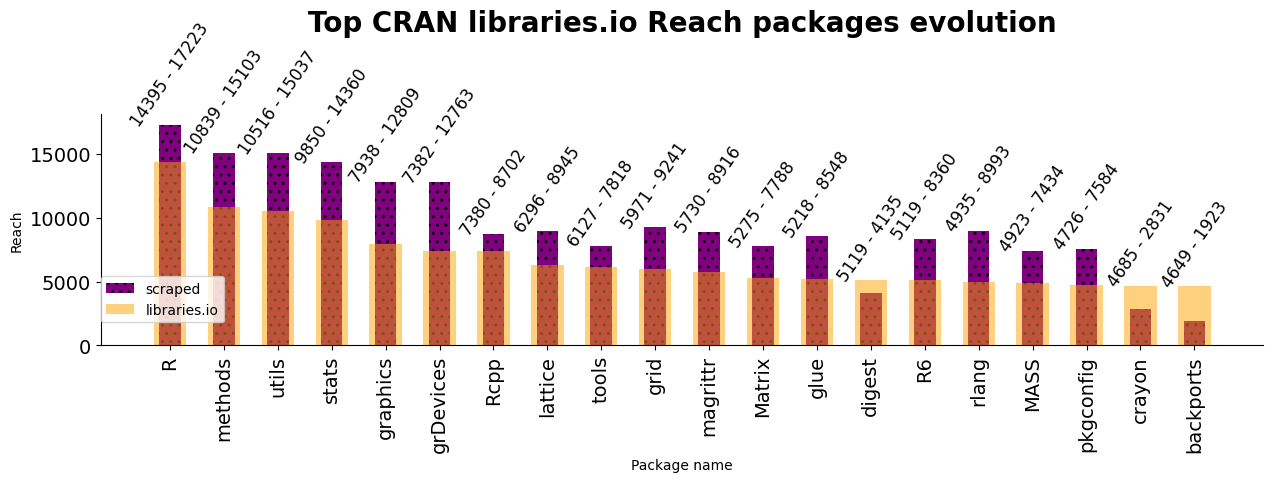
\includegraphics[width=1\textwidth]{img/cran/reach_top.png}
        \caption{Top paquetes con mayor \textit{Reach} en Libraries.io}
        \label{fig:Top reach Libraries.io}
    \end{center}
\end{figure}

\begin{figure}[ht!]
    \begin{center}
        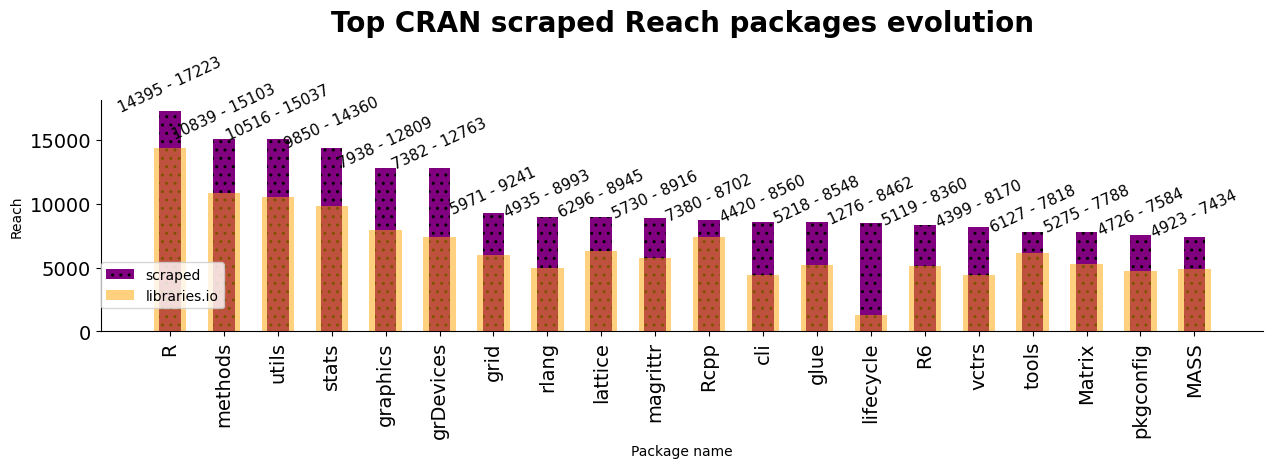
\includegraphics[width=1\textwidth]{img/cran/reach_top2.png}
        \caption{Incremento de \textit{Reach}}
        \label{fig:Top reach Scraped}
    \end{center}
\end{figure}

Si observamos los paquetes con mayor incremento en \textit{Reach} \ref{tab:Top 10 paquetes con mayor incremento en Reach}
podemos ver que la mayoría estan presentes en el top, esta tabla nos da una idea de durante este periodo
de tiempo que paquetes han ganado más dependientes.

\begin{table}[ht!]
    \begin{center}
        \begin{tabular}{|c|c|c|c|}
            \hline
            \textbf{Paquete} & \textbf{Libraries.io} & \textbf{Scraped} & \textbf{increment} \\
            \hline
            lifecycle        & 1276                  & 8462             & 7186               \\
            grDevices        & 7382                  & 12763            & 5381               \\
            farver           & 48                    & 5020             & 4972               \\
            graphics         & 7938                  & 12809            & 4871               \\
            isoband          & 5                     & 4726             & 4721               \\
            utils            & 10516                 & 15037            & 4521               \\
            stats            & 9850                  & 14360            & 4510               \\
            splines          & 2016                  & 6466             & 4450               \\
            generics         & 457                   & 4895             & 4438               \\
            methods          & 10839                 & 15103            & 4264               \\
            \hline
        \end{tabular}
        \caption{Top 10 paquetes con mayor incremento en \textit{Reach}}
        \label{tab:Top 10 paquetes con mayor incremento en Reach}
    \end{center}
\end{table}

Es curioso ver que el paquete \textit{isoband} haya incrementado tanto su \textit{Reach}.
Este paquete es una implementación de la generación de bandas de confianza para curvas y mapas de contorno.
Resulta que este paquete fue protagonista de un incidente en el pasado:

El paquete \textit{isoband} estuvo en riesgo de ser archivado en \textit{CRAN}. La razón por la que este incidente causó
revuelo es que isoband es una dependencia de \textit{ggplot2} y cuando un paquete es eliminado de \textit{CRAN}, todos los
demás paquetes que dependen de él también son eliminados. Si isoband hubiera caído, \textit{ggplot2} estaría en
riesgo. Y esto habría desencadenado la eliminación de aún más paquetes. En total, la eliminación de
isoband habría llevado a la eliminación de 4747 paquetes\cite{r-bloggers_isoband_incident}.
Afortunadamente los desarrolladores de isoband pudieron solucionar el problema y el paquete no fue eliminado.
\cite{isoband_issue}.

Luego este incremento en el \textit{Reach} puede ser debido a que los desarrolladores de paquetes que dependen de isoband
se estan reenganchando al proyecto y actualizando sus paquetes para que sigan funcionando correctamente depues del incidente.



Por último mostramos la distribucion de incremento de \textit{Reach} \ref{fig:Incremento de Reach}.

\begin{figure}[ht!]
    \begin{center}
        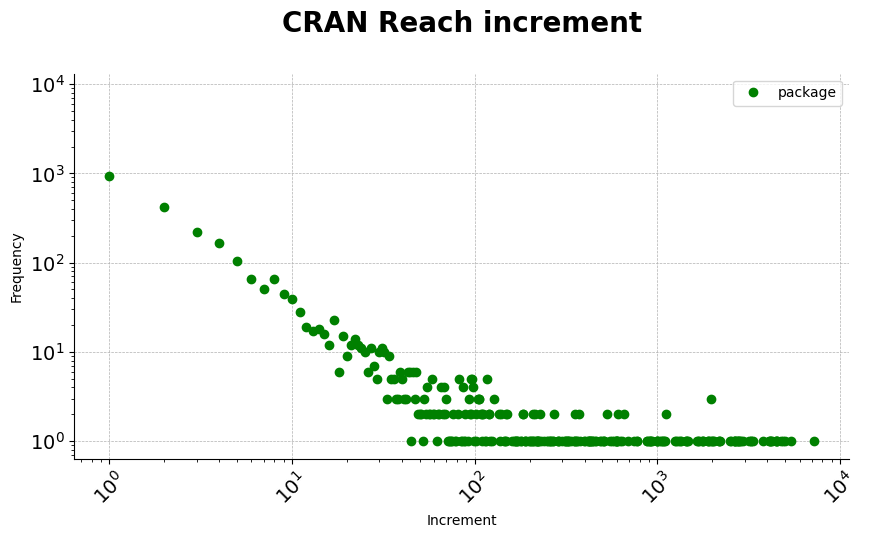
\includegraphics[width=0.8\textwidth]{img/cran/reach_increment.png}
        \caption{Incremento de \textit{Reach}}
        \label{fig:Incremento de Reach}
    \end{center}
\end{figure}


\newpage

\section{La red de dependencias de Bioconductor}

El repositorio \textit{Bioconductor} para R es una plataforma científica de código abierto que ofrece
herramientas y paquetes especializados para el análisis y la interpretación de datos genómicos.
Surgió en 2001 para abordar desafíos específicos de la biología computacional y la genómica.
\textit{Bioconductor} es reconocido por su calidad, diversidad y enfoque colaborativo. Proporciona
herramientas estadísticas y bioinformáticas para el análisis de expresión génica, variantes genéticas y más.
Su importancia radica en su contribución al avance de la investigación genómica y promoción de la
reproducibilidad y transparencia científica en el campo de la genómica y la biología computacional.

El análisis de \textit{Bioconductor} es necesario como complemento al análisis de CRAN debido a que se
enfoca específicamente en el análisis de un subconjunto del ecosistema R. Mientras que CRAN es el
repositorio principal de paquetes para el lenguaje de programación R, \textit{Bioconductor} se centra
en ofrecer herramientas especializadas para el análisis de datos genómicos y biológicos.

Además, es importante destacar que, en el contexto de \textit{Bioconductor}, se ha enfrentado el
desafío de la falta de datos de referencia en \textit{Libraries.io}, un repositorio de información
sobre paquetes de software. Esto ha llevado a la necesidad de abrir nuevos caminos y proporcionar
un conjunto de datos que no existía previamente. Al hacerlo, se está facilitando el análisis y el
estudio de los paquetes de \textit{Bioconductor}, y se está contribuyendo a la disponibilidad de
datos valiosos para la comunidad.

\subsection{El tamaño}

La red de \textit{Bioconductor} es una red relativamente pequeña\ref{tab:Medidas de la red de dependencias de Bioconductor}
en comparación con los valores de las otras redes que hemos analizado.
Los valores de las métricas indican una red de dependencias de \textit{Bioconductor} de tamaño bajo,
con alta conectividad entre los nodos.

\begin{table}[ht!]
    \begin{center}
        \begin{tabular}{|l|c|}
            \hline
            \textbf{Medida}                & \textbf{Valor} \\
            \hline
            Number of nodes                & 3509           \\
            Number of edges                & 28320          \\
            Average degree                 & 16.14          \\
            Average clustering coefficient & 0.077          \\
            \hline
        \end{tabular}
        \caption{Medidas de la red de dependencias de Bioconductor}
        \label{tab:Medidas de la red de dependencias de Bioconductor}
    \end{center}
\end{table}

El coeficiente de agrupamiento promedio de aproximadamente 0.0776 sugiere que la red tiene un nivel moderado de agrupamiento.
Esto implica que algunos nodos están conectados en grupos o comunidades, pero no existe una fuerte tendencia hacia la formación
de comunidades densamente interconectadas en toda la red. Esto puede indicar que existen diferentes grupos temáticos o
funcionales dentro de la red de dependencias de \textit{Bioconductor}, pero también existen conexiones entre estos grupos.
Este coeficiente de agrupamiento es mucho menor que el de \textit{CRAN}, que era de 0.15.

Respecto al grado medio podemos decir que es un poco mayor que el de \textit{CRAN},
para el que teniamos un valor de 12.13.

\subsection{El grado}

A la vista de la distribución de \emph{grado} \ref{fig:bioconductor_degree_dist}, se puede observar una distribución
de \emph{ley de potencia}, lo cual es común en las \emph{redes de dependencias}.
En la gráfica, se puede apreciar que a partir de un \emph{grado} de 50, el
número de \emph{nodos} comienza a reducirse de manera exponencial, quedando
sólo unos pocos representantes. Como era de esperar, se observan \emph{hubs}
o \emph{nodos de alto grado}, con valores cercanos a 2000. Esta presencia
de \emph{hubs} indica la existencia de elementos altamente conectados que
desempeñan un papel crucial en la estructura de la red de dependencias.

\begin{figure}[ht!]
    \begin{center}
        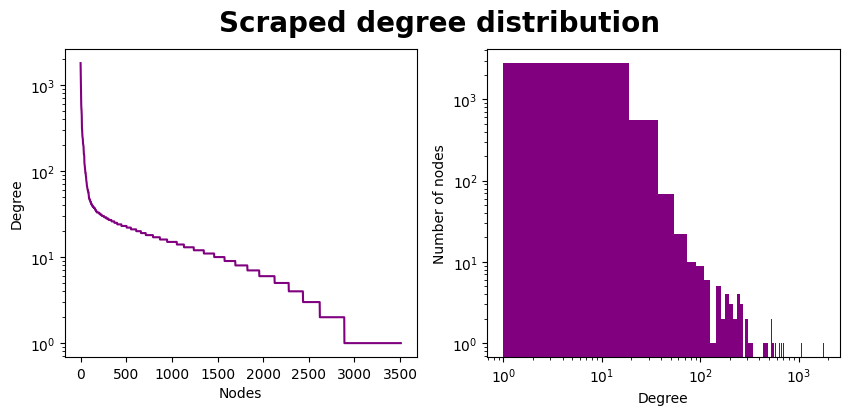
\includegraphics[width=1\textwidth]{img/bioconductor/degree_dist.png}
        \caption{Distribución de grado de la red de dependencias de Bioconductor}
        \label{fig:bioconductor_degree_dist}
        \caption{Distribución de grado de la red de dependencias de Bioconductor}
    \end{center}
\end{figure}

\subsubsection{El grado de salida \textit{Out degree}}

La distribución del \emph{grado de salida} en la red analizada presenta similitudes con
la distribución de la red de CRAN. En este caso, el \emph{grado de salida máximo} es
notablemente inferior debido al menor tamaño de la red, pero la tendencia general es
similar. Se puede apreciar que a partir de un \emph{grado de salida} de 10, la frecuencia
de individuos en la red se reduce significativamente. La mayoría de los nodos tienen un
\emph{grado de salida} inferior a 10, siendo estos el grupo más numeroso en la red.\ref{fig:bioconductor_out_degree_dist}

\begin{figure}[ht!]
    \begin{center}
        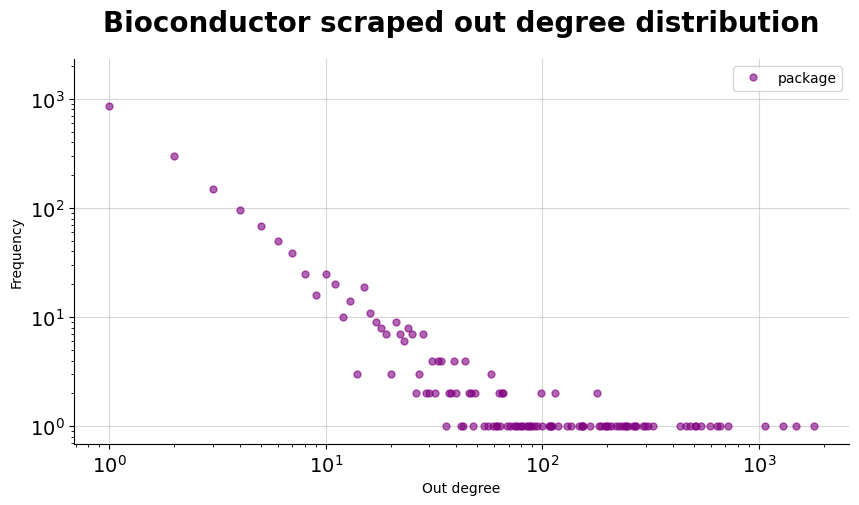
\includegraphics[width=0.8\textwidth]{img/bioconductor/out_degree_dist.png}
        \caption{Distribución de grado de salida de la red de dependencias de Bioconductor}
        \label{fig:bioconductor_out_degree_dist}
    \end{center}
\end{figure}

En cuanto a los paquetes que representan el \emph{mayor grado de salida}\ref{fig:bioconductor_out_degree}
en la red analizada, se observa que la mayoría de ellos también aparecen en el \emph{top} de la red de CRAN.
Este hallazgo es coherente, dado que, como se mencionó anteriormente, Bioconductor es un
subconjunto de los paquetes de R, y es esperable que estos paquetes tengan una importancia
similar en ambos repositorios.
Además, se observa que en este \emph{top} se encuentran los paquetes más importantes y exclusivos
de Bioconductor, como BiocGenerics o Biobase, entre otros. Esto nos indica que la red de Bioconductor
está especializada en el ámbito de la bioinformática, ya que estos paquetes desempeñan un papel crucial
en el análisis y procesamiento de datos biológicos. Su presencia en el \emph{top} indica la importancia
de la especialización de Bioconductor en este campo.

\begin{figure}[ht!]
    \begin{center}
        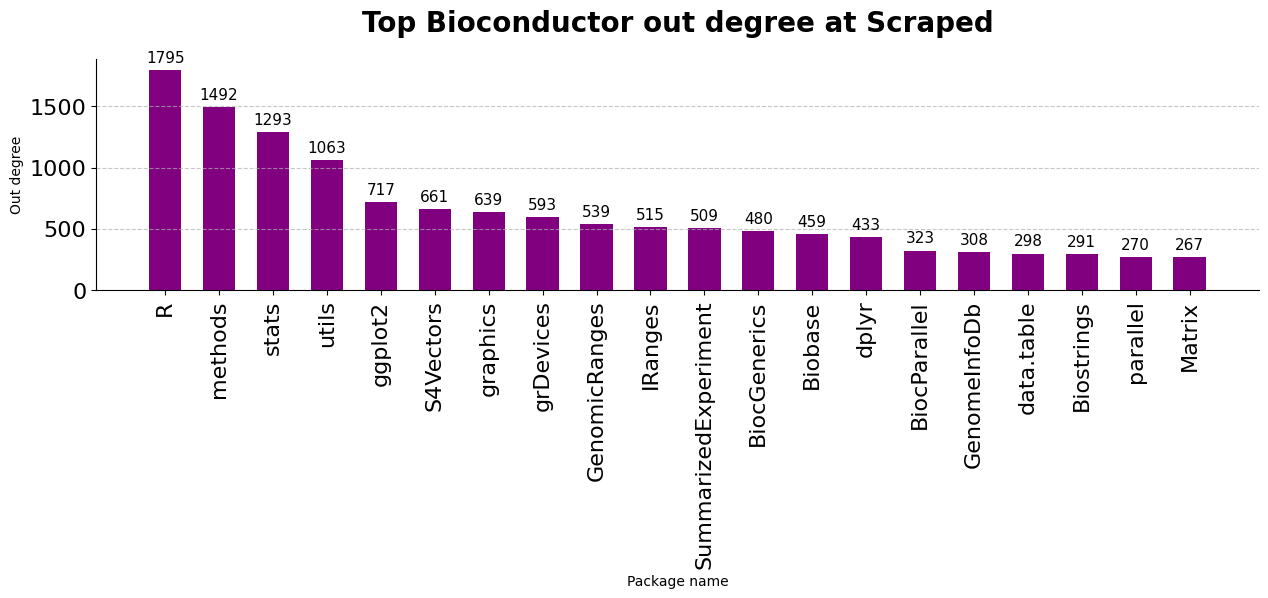
\includegraphics[width=1\textwidth]{img/bioconductor/top_out_degree.png}
        \caption{Top 10 de los paquetes con mayor grado de salida en la red de dependencias de Bioconductor}
        \label{fig:bioconductor_out_degree}
    \end{center}
\end{figure}


\subsubsection{El grado de entrada \textit{In degree}}

La distribución de \emph{in degree}\ref{fig:bioconductor_in_degree_dist} en la red de Bioconductor muestra algunas diferencias con respecto
a la red de CRAN. Se observa que hay un menor número de nodos en la red de Bioconductor en comparación
con CRAN. Además, la frecuencia máxima de nodos con \emph{in degree} ya no se encuentra en los valores
1 o 2, como ocurre en CRAN. En Bioconductor, se puede apreciar que hay más nodos con \emph{in degree}
en el rango de 10 a 20 en comparación con aquellos con un valor de 1.

Otro aspecto a tener en cuenta es que el \emph{in degree} máximo en la red de Bioconductor tiene un
valor de 85, mientras que en CRAN el valor máximo es de 50. Esto indica que en Bioconductor existen
nodos con un mayor número de dependencias entrantes, lo que podría reflejar la complejidad y la
interconexión de los paquetes en Bioconductor. Estas diferencias en la distribución de \emph{in degree}
evidencian las particularidades y características propias de la red de Bioconductor en comparación con
la red de CRAN.

\begin{figure}[ht!]
    \begin{center}
        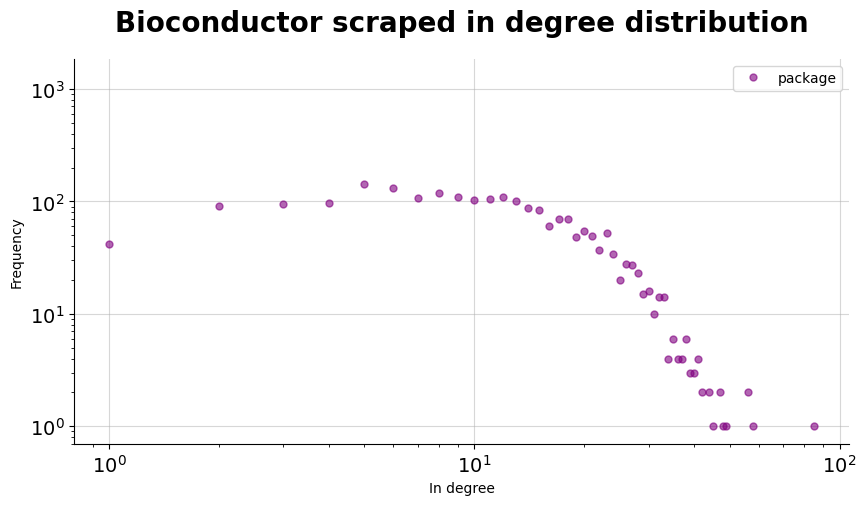
\includegraphics[width=0.8\textwidth]{img/bioconductor/in_degree_dist.png}
        \caption{Distribución de grado de entrada de la red de dependencias de Bioconductor}
        \label{fig:bioconductor_in_degree_dist}
    \end{center}
\end{figure}

Los paquetes que se encuentran en el \emph{top} de \emph{grado de entrada} \ref{fig:bioconductor_in_degree} son aquellos que presentan
un mayor número de dependencias en la red, sin tener en cuenta la transitividad de las conexiones.
Esto implica que estos paquetes son altamente dependientes de otros paquetes en la red de Bioconductor en el primer nivel de
profundidad del árbol de dependencias, lo que sugiere su importancia y relevancia en el ecosistema de Bioconductor.

\begin{figure}[ht!]
    \begin{center}
        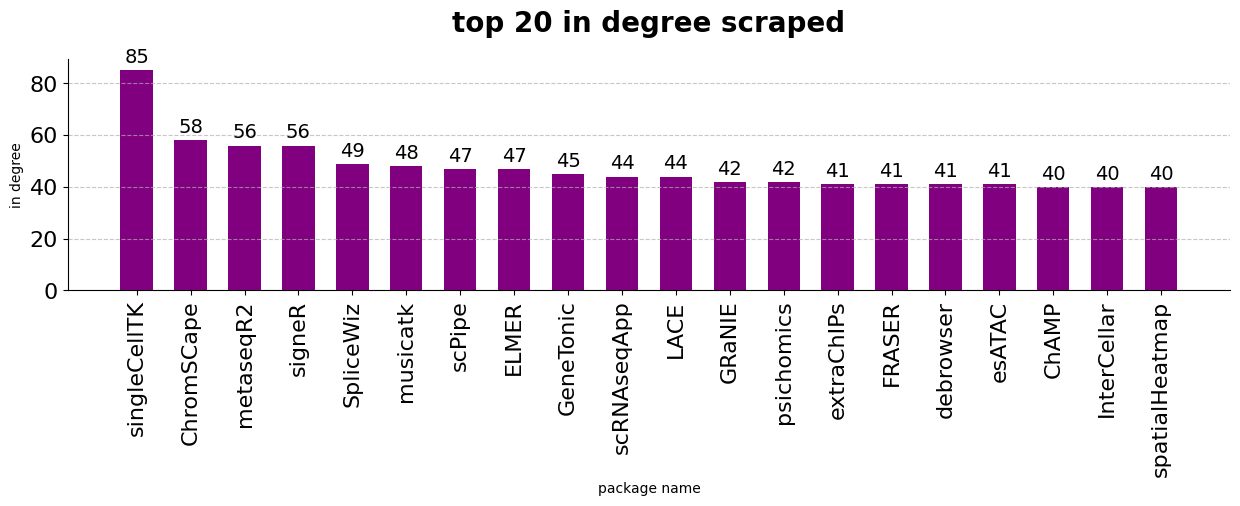
\includegraphics[width=1\textwidth]{img/bioconductor/top_in_degree.png}
        \caption{Top 10 de los paquetes con mayor grado de entrada en la red de dependencias de Bioconductor}
        \label{fig:bioconductor_in_degree}
    \end{center}
\end{figure}

\subsection{El PageRank}

La distribución de \textit{PageRank} \ref{fig:bioconductor_pagerank_dist} en la red de \textit{Bioconductor} no revela patrones claros
y sencillos de analizar. Observando el gráfico, podemos determinar que la frecuencia máxima de nodos
con el mismo valor de \textit{PageRank} se sitúa aproximadamente entre \textit{0.0002} y \textit{0.0005}.
El rango normal de valores se encuentra entre \textit{0.0002} y \textit{0.002}, aunque en algunos casos
particulares se alcanzan valores de \textit{0.003} o \textit{0.004}. Estos valores representan la importancia
relativa de los nodos en la red, teniendo en cuenta tanto las conexiones directas como las conexiones
indirectas a través de otros nodos en la red. Sin embargo, debido a la complejidad y tamaño de la red
de \textit{Bioconductor}, es necesario realizar un análisis más detallado y específico para comprender
plenamente la distribución y significado de los valores de \textit{PageRank} en esta red.
Si la comparamos con la distribución de \textit{PageRank} de la red de \textit{CRAN}, se observa que
Bioconductor tiene muchos menos paquetes despreciables, es decir, paquetes con un \textit{PageRank} muy
alto. Esto indica que en Bioconductor es más estable que en CRAN.

\begin{figure}[ht!]
    \begin{center}
        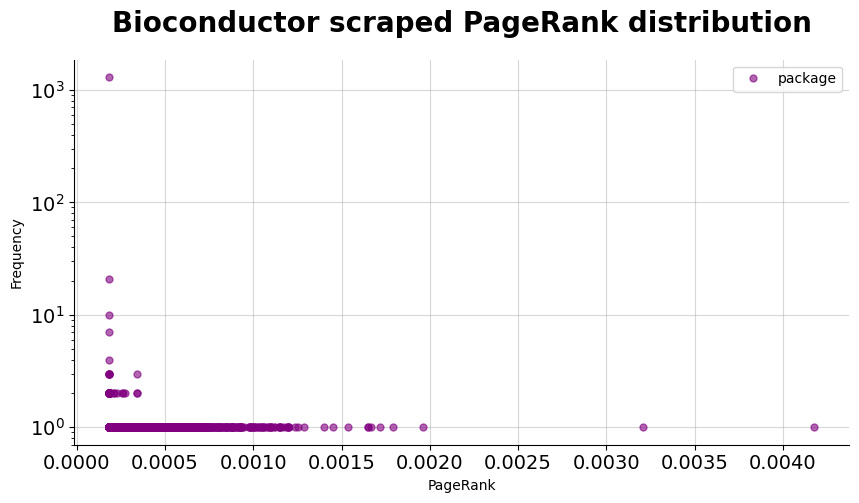
\includegraphics[width=1\textwidth]{img/bioconductor/pagerank_dist.png}
        \caption{Distribución de PageRank de la red de dependencias de Bioconductor}
        \label{fig:bioconductor_pagerank_dist}
    \end{center}
\end{figure}


Respecto al top de dependencias con mayor \textit{PageRank} \ref{fig:bioconductor_top_pagerank_dependencies},
estos paquetes representan una vulnerabilidad significativa debido a su alto \textit{in degree} de paquetes similares a el
y la transitividad que acumulan entre ellos. Desde el punto de vista
del autor, sería recomendable evitar depender de alguno de estos paquetes, ya que se encuentran en un entorno
donde la probabilidad de vulnerabilidad es mayor. La dependencia de estos paquetes puede aumentar la propagación
de posibles problemas o errores a lo largo de la red de \textit{Bioconductor}. Por lo tanto, es esencial
considerar alternativas y evaluar cuidadosamente las dependencias al desarrollar o utilizar aplicaciones
basadas en esta red.

\begin{figure}[ht!]
    \begin{center}
        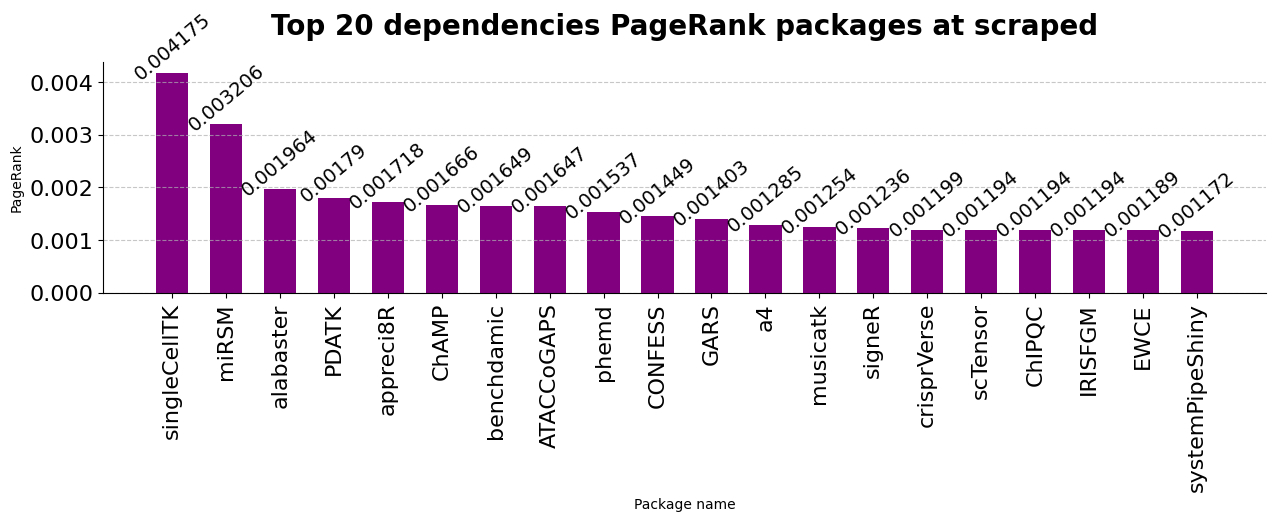
\includegraphics[width=1\textwidth]{img/bioconductor/top_pagerrank_dependencies.png}
        \caption{Top dependencias con mayor PageRank en la red de dependencias de Bioconductor}
        \label{fig:bioconductor_top_pagerank_dependencies}
    \end{center}
\end{figure}

Realizando una inversion de la red de dependencias de Bioconductor, se obtiene la red de paquetes, desde este punto de vista
el \textit{PageRank} ahora esta ponderando la importancia de los paquetes en la red, es decir, aquellos paquetes que son dependencias
de otros paquetes importantes, son considerados como los más importantes en la red. En la figura \ref{fig:bioconductor_top_pagerank_packages}
se muestran los paquetes con mayor \textit{PageRank} bajo este punto de vista de Bioconductor.

\begin{figure}[ht!]
    \begin{center}
        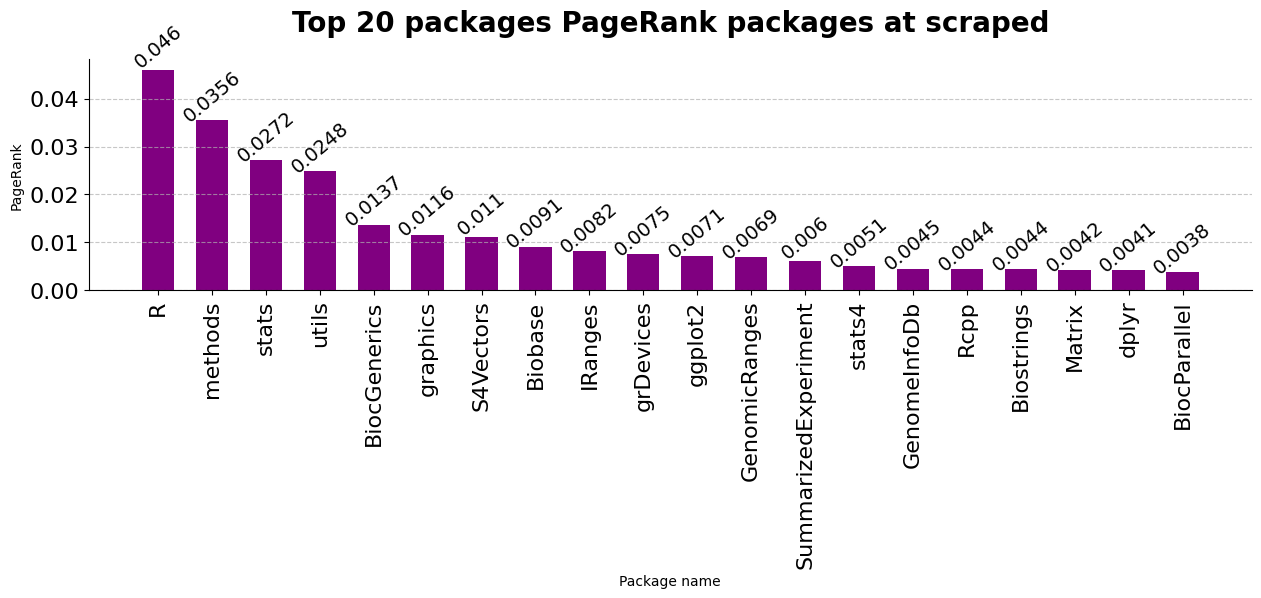
\includegraphics[width=1\textwidth]{img/bioconductor/top_pagerrank_packages.png}
        \caption{Top paquetes con mayor PageRank en la red de dependencias de Bioconductor}
        \label{fig:bioconductor_top_pagerank_packages}
    \end{center}
\end{figure}

\subsection{Impacto (Impact)}

La distribución de \textit{Impact} \ref{fig:bioconductor_impact_dist} en la red de \textit{Bioconductor} nos indica
que la mayoría de paquetes presentan un impacto bajo, es decir, no son dependencias de otros paquetes. Sin embargo,
como estamos acostumbrados, esta distribución sigue una ley de potencia, lo que nos indica que existen algunos paquetes
que presentan un impacto alto, es decir, son dependencias de muchos otros paquetes.

\begin{figure}[ht!]
    \begin{center}
        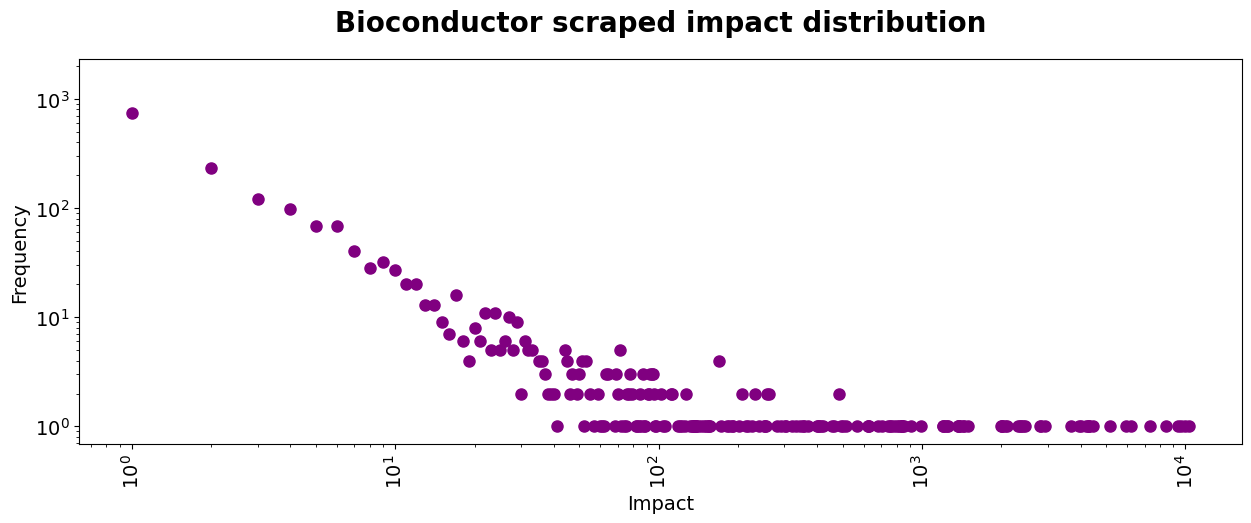
\includegraphics[width=1\textwidth]{img/bioconductor/impact.png}
        \caption{Distribución de Impact de la red de dependencias de Bioconductor}
        \label{fig:bioconductor_impact_dist}
    \end{center}
\end{figure}

A continuación se muestran los paquetes con mayor impacto en la red de dependencias de Bioconductor. \ref{tab:bioconductor_top_impact}

\begin{table}[ht!]
    \centering
    \small
    \label{tab:bioconductor_top_impact}
    \begin{tabular}{|l|c|}
        \hline
        \textbf{Paquete} & \textbf{Impacto} \\
        \hline
        R                & 10284            \\
        methods          & 9933             \\
        stats            & 9617             \\
        utils            & 9371             \\
        graphics         & 8398             \\
        BiocGenerics     & 7357             \\
        stats4           & 6235             \\
        S4Vectors        & 5942             \\
        IRanges          & 5149             \\
        RCurl            & 4450             \\
        GenomeInfoDbData & 4302             \\
        GenomeInfoDb     & 4298             \\
        tools            & 4268             \\
        zlibbioc         & 4198             \\
        XVector          & 4023             \\
        grDevices        & 3927             \\
        Biobase          & 3661             \\
        GenomicRanges    & 2922             \\
        matrixStats      & 2831             \\
        Matrix           & 2800             \\
        \bottomrule
    \end{tabular}
    \caption{Paquetes de Bioconductor con más impacto}
\end{table}


Como se puede apreciar en esta tabla, los paquetes con mayor impacto son paquetes que estan representando puestos altos
respecto a las métricas de \textit{Out degree} y \textit{PageRank}, lo que nos indica que estos paquetes son importantes en la red ya que son
necesarios por otros paquetes para funcionar.
En el caso opuesto, los paquetes con menor impacto son paquetes que no son dependencias de otros paquetes, por lo que tienen
un impacto de 0.


\newpage

\section{La red de dependencias de PyPI}

En el ámbito del lenguaje de programación \textit{Python}, nos enfocamos en el análisis de \textit{PyPI}
(\textit{Python Package Index}). \textit{PyPI} es un repositorio ampliamente adoptado en la comunidad de
\textit{Python} debido a su facilidad de uso, su naturaleza de código abierto y su extensa colección de
paquetes.\footnote{Es importante mencionar que existen otros repositorios interesantes como \textit{Conda}.}

La facilidad de uso de \textit{PyPI} se deriva de su diseño intuitivo y las funcionalidades que ofrece
para la gestión de paquetes en \textit{Python}. Los desarrolladores pueden acceder a \textit{PyPI} como
una fuente centralizada para descubrir, descargar e instalar una amplia variedad de paquetes y bibliotecas
desarrollados por la comunidad.

\subsection{Tamaño de la red}

En el análisis comparativo entre los datos proporcionados por \textit{Libraries.io} y los recolectados en
este trabajo, se ha revelado una sorprendente tendencia en el número de paquetes presentes en \textit{PyPI}.
Se ha observado un aumento significativo en la cantidad de paquetes disponibles en \textit{PyPI} en
comparación con datos anteriores.

Este hallazgo sugiere un crecimiento notable en el ecosistema de paquetes de \textit{Python} y evidencia
el interés y participación de la comunidad en \textit{PyPI}. Este aumento en el número de paquetes puede
ser atribuido a diversos factores, como la creciente popularidad de \textit{Python} como lenguaje de
programación, el aumento en la adopción de \textit{Python} en diferentes campos de aplicación y el
creciente número de contribuyentes que comparten sus proyectos y soluciones a través de \textit{PyPI}.


\begin{figure}[ht!]
    \begin{center}
        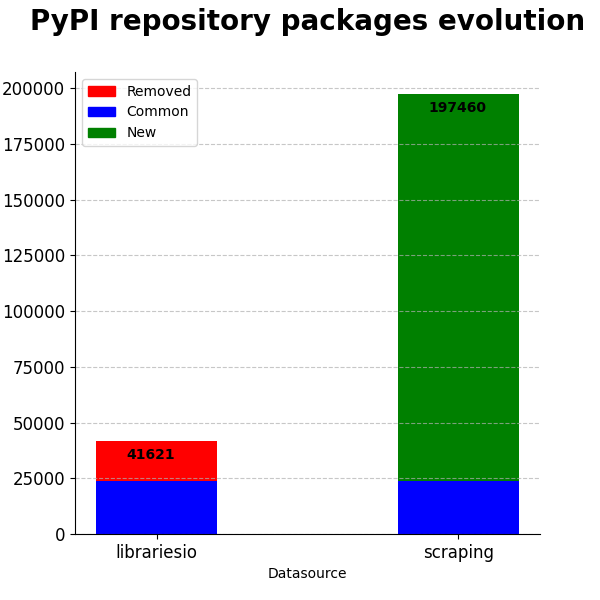
\includegraphics[width=0.6\textwidth]{img/pypi/bar_common_packages.png}
        \caption{Comparación de la cantidad de paquetes en PyPI entre los datos de Libraries.io (2020) y los recolectados en este trabajo (2023).}
        \label{fig:pipy_common_packages_bar}
    \end{center}
\end{figure}

\begin{figure}[ht!]
    \begin{center}
        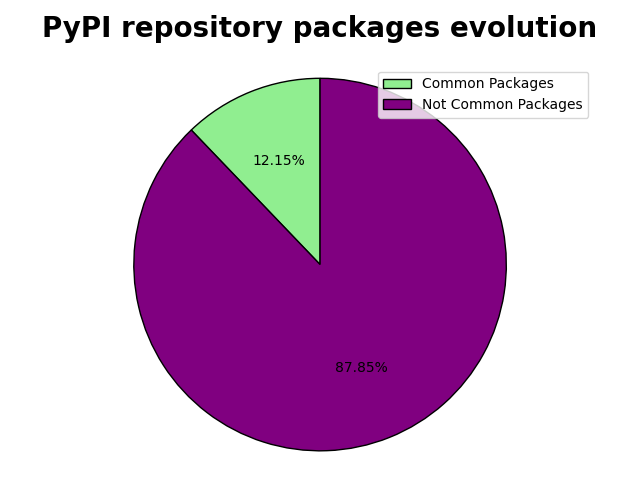
\includegraphics[width=0.6\textwidth]{img/pypi/circ_common_packages.png}
        \caption{Paquetes comunes y no comunes entre los datos de Libraries.io (2020) y los recolectados en este trabajo (2023).}
        \label{fig:pipy_common_packages_circle}
    \end{center}
\end{figure}

El análisis de los datos revela que aproximadamente el \textit{57 \%} de los paquetes que estaban
presentes en el conjunto de datos antiguo de PyPI se han mantenido en el nuevo conjunto de datos
\footnote{Este porcentaje se basa en datos obtenidos experimentalmente.}. Este porcentaje
relativamente elevado indica que la red de paquetes en PyPI ha logrado mantener una cantidad considerable
de paquetes de manera estable a lo largo del tiempo \ref{tab:pypi_common_packages}.

\begin{table}[ht!]
    \begin{center}
        \begin{tabular}{|l|r|}
            \hline
            \textbf{Descripción}                               & \textbf{Cantidad} \\
            \hline
            Paquetes en Libraries.io                           & 41,621            \\
            Paquetes en Scraped                                & 197,460           \\
            Paquetes comunes                                   & 24,001            \\
            Paquetes de Libraries.io no disponibles en Scraped & 17,620            \\
            Paquetes en Scraped que no estan en Libraries.io   & 173,459           \\
            \hline
        \end{tabular}
    \end{center}
    \label{tab:pypi_common_packages}
    \caption{Comparación de paquetes en PyPI entre los datos de Libraries.io (2020) y los recolectados en este trabajo (2023).}
\end{table}

Es importante destacar que este conjunto de paquetes que se ha mantenido representa aproximadamente
el \textit{12.15\%} del total de paquetes disponibles en PyPI en la actualidad. Esta proporción
da una idea de la estabilidad relativa de la red, ya que una parte significativa de los
paquetes ha logrado mantener su presencia en PyPI a pesar de los posibles cambios y
actualizaciones\footnote{Los datos se refieren al momento de la última actualización y pueden estar
    sujetos a cambios futuros.}.

\begin{figure}[ht!]
    \begin{center}
        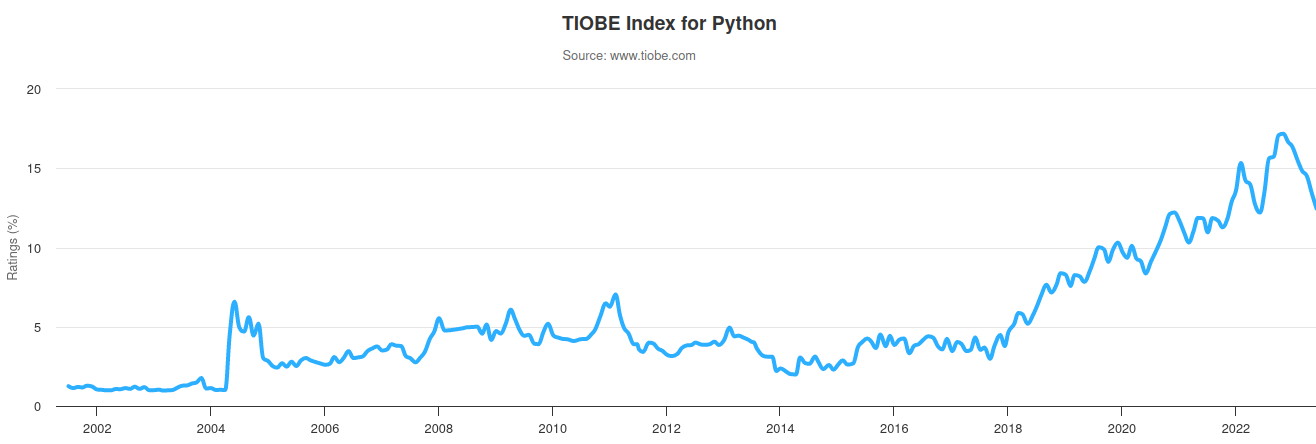
\includegraphics[width=1\textwidth]{img/pypi/pypi_popularity.png}
        \caption{Popularidad de Python a lo largo del tiempo.}
        \label{fig:pypi_popularity}
    \end{center}
\end{figure}


Esta tendencia en la popularidad de Python se ve reflejada en las estadísticas realizadas por la
empresa TIOBE \ref{fig:pypi_popularity}\footnote{\url{https://www.tiobe.com/tiobe-index/python/}}.


\subsection{Grado de la red}

Al examinar la distribución de grado en ambos conjuntos de datos, se observa que sigue una distribución
de ley de potencias\footnote{La distribución de ley de potencias es una característica común en las redes
    de dependencias.} \cite{enwiki:1160892030}.

Al analizar el gráfico, se evidencia que el grado máximo alcanzado por un paquete ha
experimentado un incremento significativo. Tomando como punto de referencia el número de nodos con grado
\textit{1000}, se puede apreciar una diferencia sustancial entre la red de \textit{Libraries.io} y los
nuevos datos recolectados. Mientras que en \textit{Libraries.io} se registran menos de \textit{10} paquetes
con dicho grado, en los nuevos datos se han identificado aproximadamente \textit{40} individuos
\footnote{Estos datos se basan en el análisis realizado en una fecha específica y pueden estar sujetos
    a cambios en el tiempo.}.

\begin{figure}[ht!]
    \begin{center}
        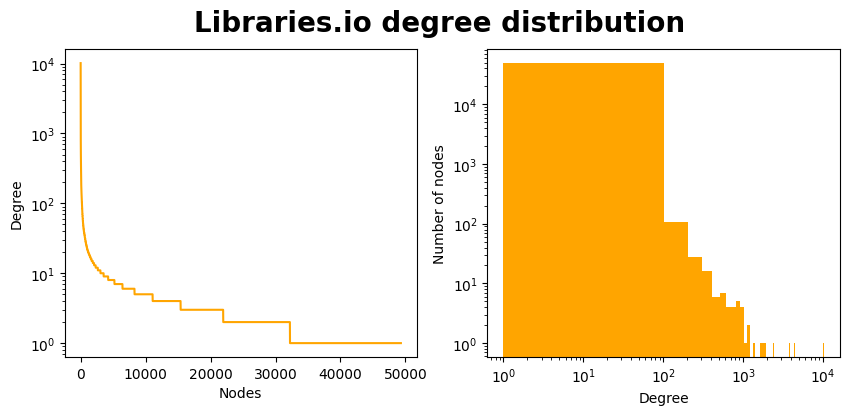
\includegraphics[width=0.8\textwidth]{img/pypi/librariesio_degree_distribution.png}
        \caption{Distribución de grado de PyPI para Libraries.io.}
        \label{fig:pypi_librariesio_degree_distribution}
    \end{center}
\end{figure}

\begin{figure}[ht!]
    \begin{center}
        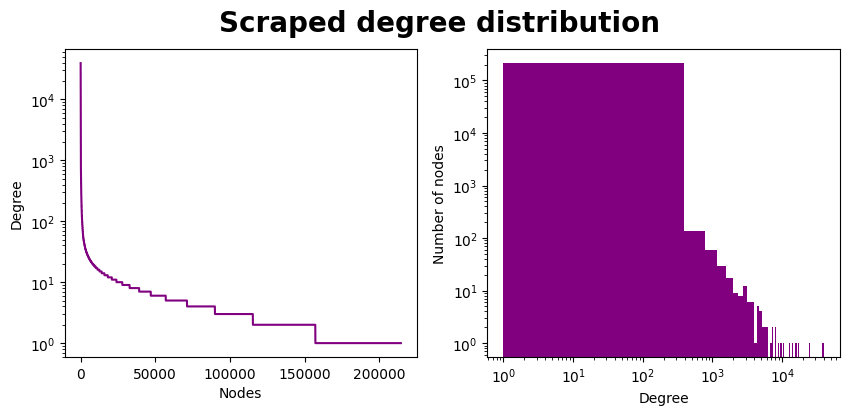
\includegraphics[width=0.8\textwidth]{img/pypi/scraped_degree_distribution.png}
        \caption{Distribución de grado de PyPI para los datos recolectados en este trabajo (2023).}
        \label{fig:pypi_scraped_degree_distribution}
    \end{center}
\end{figure}

Además, al calcular el grado promedio de los grafos correspondientes a \textit{Libraries.io} y el nuevo
conjunto, se obtiene un valor de \textit{2.73} y \textit{4.35}, respectivamente. Estos valores indican
que, en promedio, cada paquete en la red de \textit{Libraries.io} está conectado a alrededor de
\textit{2.73} otros paquetes, mientras que en los nuevos datos, cada paquete está conectado a
aproximadamente \textit{4.35} otros paquetes.

Estas estadísticas revelan cambios importantes en la estructura de la red de dependencias de paquetes.
El incremento en el grado máximo y el aumento en el grado promedio indican una mayor interconectividad
y complejidad en la red, lo cual puede ser atribuido al crecimiento y la evolución del ecosistema de
paquetes en Python.

Es importante destacar que la distribución de ley de potencias y la presencia de paquetes con grados
altos en la red tienen implicaciones significativas en términos de la propagación de dependencias y la
influencia de ciertos paquetes en la comunidad.

\subsubsection{Grado de salida (\textit{Out degree})}

El \textit{out degree} es una métrica que proporciona información
sobre el número de dependientes de un paquete dado. En el contexto de \textit{Libraries.io},
analizando los datos, podemos identificar los paquetes que tienen más dependientes, es decir,
los que están en el \textit{Top} de las dependencias más utilizadas.

Los resultados obtenidos revelan una tendencia general en la cual las dependencias más populares han
experimentado un aumento en su popularidad, siendo ahora requeridas por un mayor número de paquetes
en la red de dependencias. En particular, se observa un incremento significativo en la popularidad
de las bibliotecas \textit{requests}, \textit{numpy}, \textit{pandas} y \textit{pytest} en comparación
con otros paquetes presentes en este ranking.

Estos hallazgos indican que estas bibliotecas han adquirido una mayor relevancia y utilidad en el
desarrollo de proyectos y aplicaciones en el entorno de Python.

\begin{figure}[ht!]
    \begin{center}
        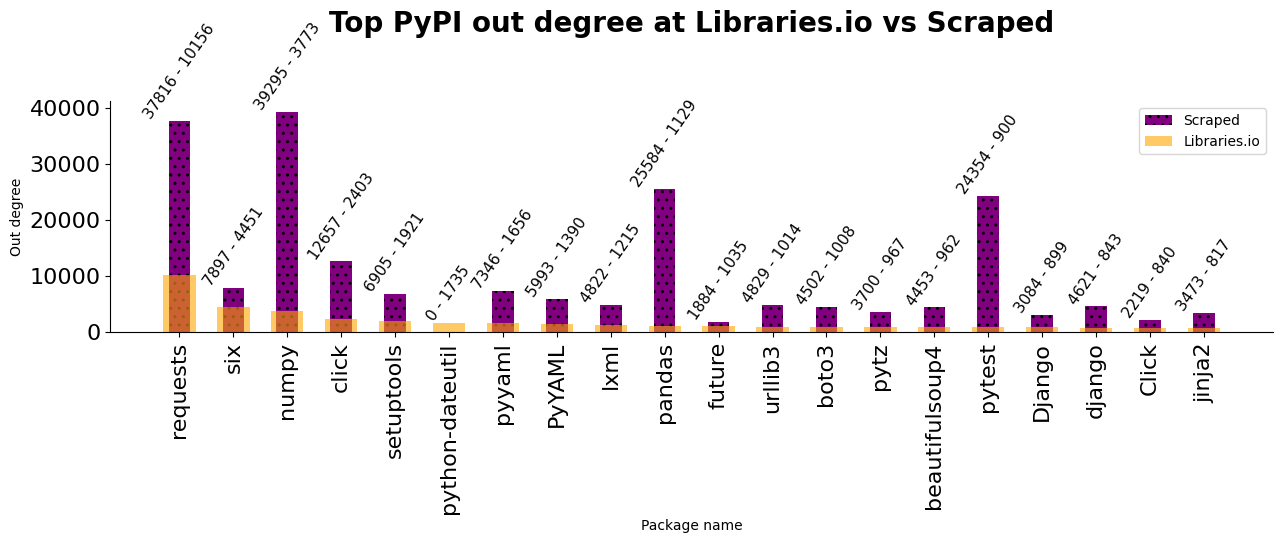
\includegraphics[width=1\textwidth]{img/pypi/libio_t20_outd_comparison.png}
        \caption{Top de paquetes con mayor grado de salida en PyPI para Libraries.io (2020).}
        \label{fig:pypi_libio_outd_comparison}
    \end{center}
\end{figure}

\begin{figure}[ht!]
    \begin{center}
        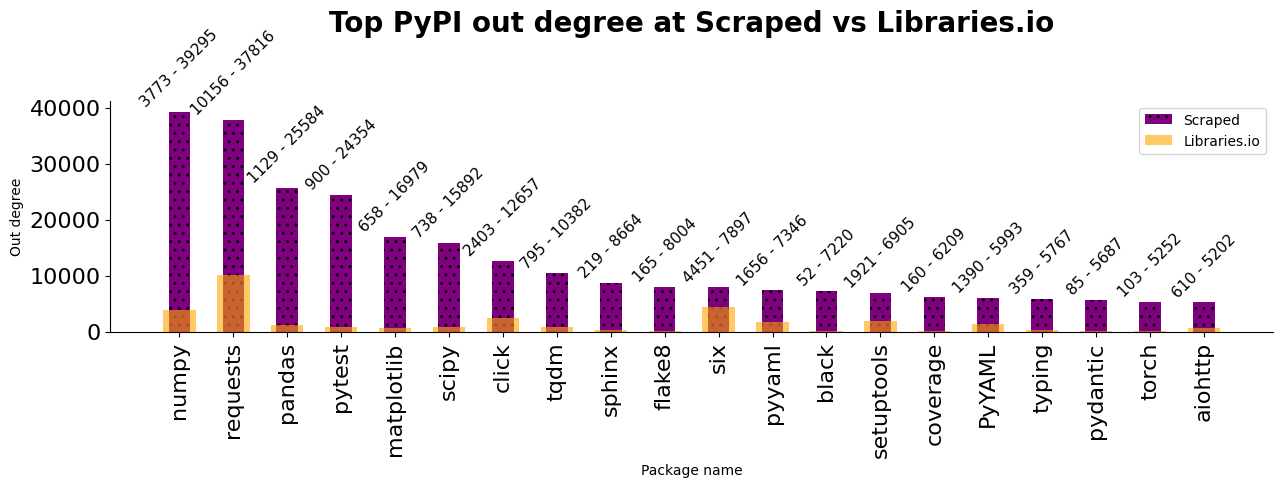
\includegraphics[width=1\textwidth]{img/pypi/libio_scraped_t20_comparation.png}
        \caption{Top de paquetes con mayor grado de salida en PyPI para Scraped (2023).}
        \label{fig:pypi_scraped_outd_comparison}
    \end{center}
\end{figure}

En este análisis de ranking, se observa que ciertos paquetes se han mantenido con respecto al ranking
anterior, lo cual indica su relevancia a lo largo del tiempo. Estos
paquetes incluyen \textit{PyYAML}, \textit{click}, \textit{numpy}, \textit{pandas}, \textit{pytest},
\textit{pyyaml}, \textit{requests}, \textit{setuptools} y \textit{six}. Su presencia continua en el
ranking sugiere que son dependencias fundamentales y ampliamente utilizadas en proyectos y aplicaciones
de Python\footnote{La relevancia y utilidad de estos paquetes se basa en la percepción de la comunidad
    de desarrolladores de Python y puede variar dependiendo del contexto y los requisitos del proyecto}.

Por otro lado, se identifican paquetes que han ascendido en el ranking en comparación con la clasificación
anterior. Estos paquetes incluyen \textit{black}, \textit{coverage}, \textit{flake8}, \textit{matplotlib},
\textit{odoo}, \textit{python}, \textit{scikit}, \textit{scipy}, \textit{sphinx}, \textit{tqdm} y
\textit{typing}. Su ascenso en el ranking puede ser atribuido a su creciente popularidad y utilidad en el
desarrollo de proyectos de Python, ya que son bibliotecas ampliamente conocidas y utilizadas por la
comunidad de desarrolladores\footnote{El ascenso en el ranking puede deberse a mejoras en funcionalidad,
    adopción en proyectos populares u otros factores que influyen en su popularidad}.

Por último, se muestra la distribución de \textit{out degree} para ambos conjuntos de datos \ref{fig:pypi_libio_outd_dist} \ref{fig:pypi_scraped_outd_dist}

\begin{figure}[ht!]
    \begin{center}
        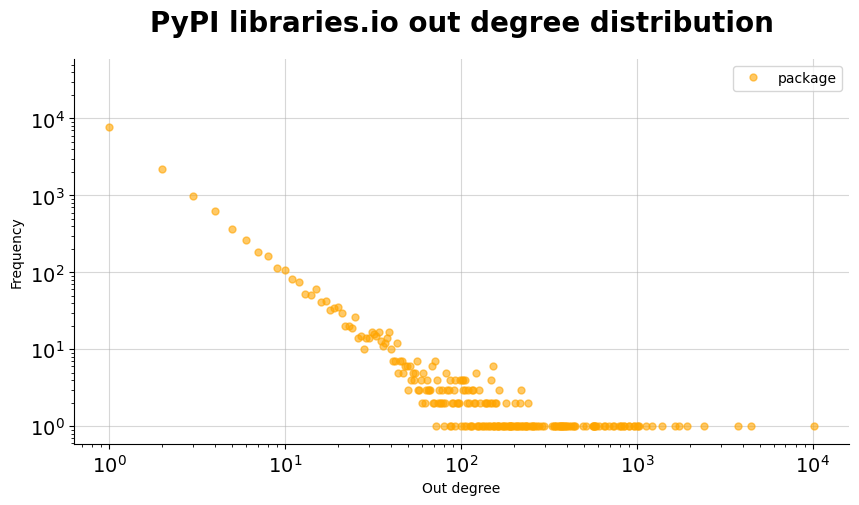
\includegraphics[width=0.8\textwidth]{img/pypi/outd_libio_dist.png}
        \caption{Distribución de \textit{Out degree} para Libraries.io (2020)}
        \label{fig:pypi_libio_outd_dist}
    \end{center}
\end{figure}

\begin{figure}[ht!]
    \begin{center}
        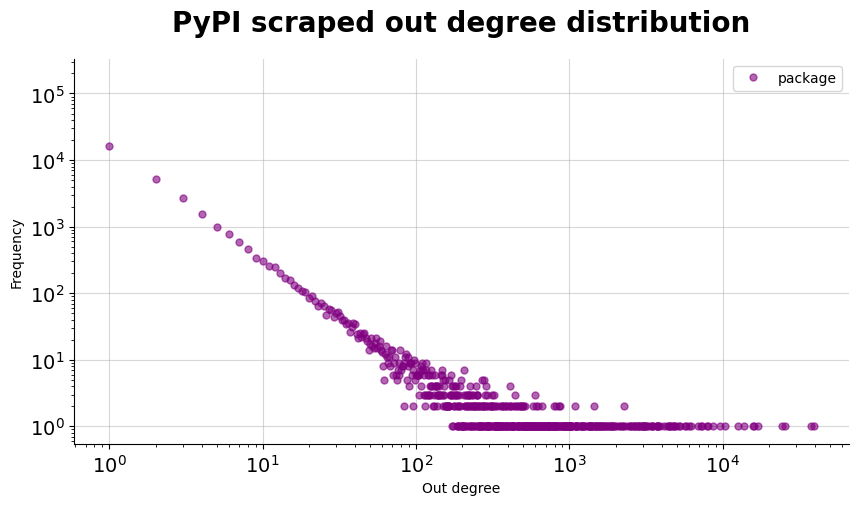
\includegraphics[width=0.8\textwidth]{img/pypi/outd_scraped_dist.png}
        \caption{Distribución de \textit{Out degree} para Scraped (2023)}
        \label{fig:pypi_scraped_outd_dist}
    \end{center}
\end{figure}

Al analizar los gráficos de las distribuciones de \textit{out degree}, se observa una tendencia similar
en ambos conjuntos. Se evidencia un incremento general en el número total de paquetes, lo que indica un
crecimiento continuo en el ecosistema de paquetes.

Se ha observado un aumento en el número de paquetes con un grado de salida bajo, lo que indica que estos
paquetes tienen menos dependencias externas. Este fenómeno puede deberse a la introducción de paquetes
más autónomos y autosuficientes en el ecosistema de Python, lo que reduce la necesidad de depender de
otros paquetes para su funcionamiento.

Por otro lado, se ha identificado un incremento \ref{fig:dependents_increase} en el grado de salida de los paquetes más populares.
Esto indica que estos paquetes están siendo cada vez más utilizados como dependencias por otros paquetes
en la comunidad de Python. Este aumento en el grado de salida de los paquetes populares puede ser atribuido
a su funcionalidad ampliamente reconocida y popularidad.

\begin{figure}[ht!]
    \begin{center}
        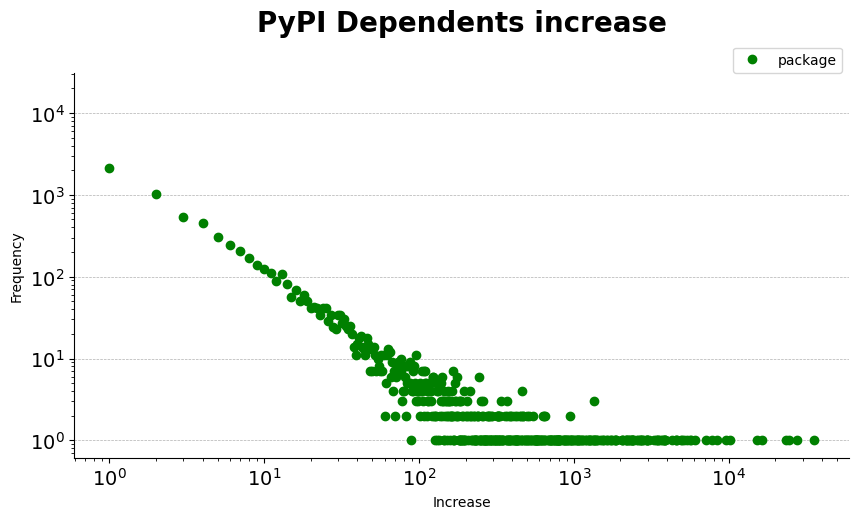
\includegraphics[width=0.8\textwidth]{img/pypi/dependents_increase.png}
        \caption{Incremento del \textit{Out degree} en PyPI (2010-2023)}
        \label{fig:dependents_increase}
    \end{center}
\end{figure}


\subsubsection{Grado de entrada (\textit{In degree})}

Esta métrica nos da una idea del número de dependencias que tiene un paquete dado.
Analizados los datos de Libraries.io y representados sobre un gráfico obtenemos los siguientes resultados: \ref{fig:pypi_libio_ind_comparison}

\begin{figure}[ht!]
    \begin{center}
        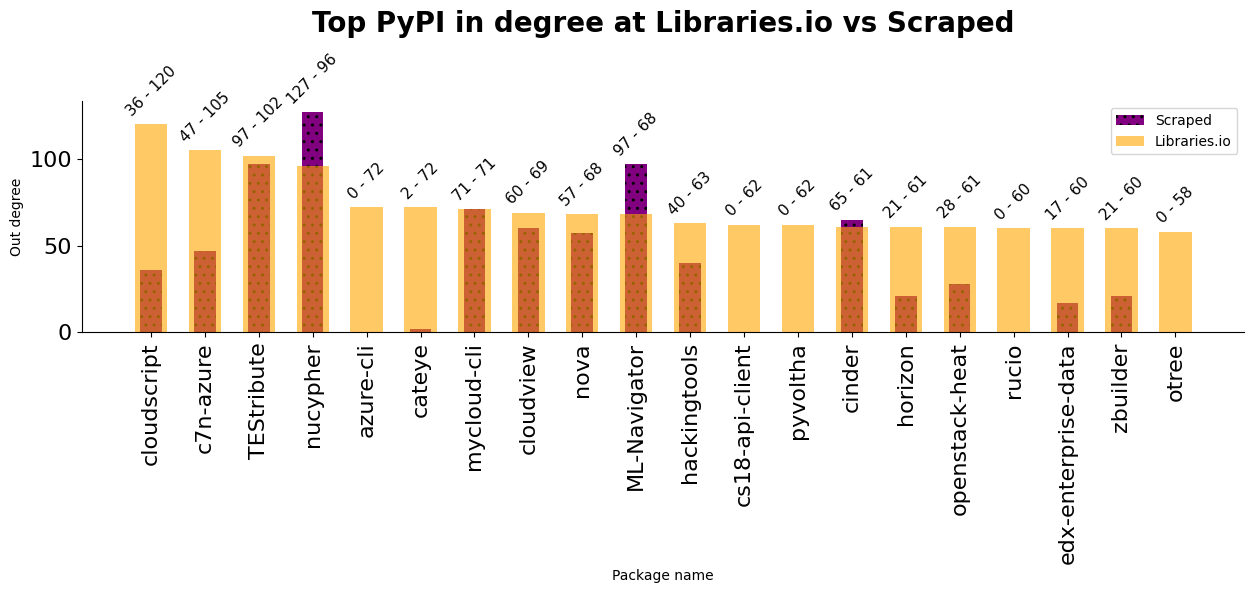
\includegraphics[width=1\textwidth]{img/pypi/libio_t20_ind_comparison.png}
        \caption{Top paquetes con mayor \textit{In degree} en Libraries.io (2020)}
        \label{fig:pypi_libio_ind_comparison}
    \end{center}
\end{figure}

Se observa una tendencia decreciente en el número de dependencias entre los paquetes con mayor \textit{In degree}
dentro del conjunto de bibliotecas de \textit{Libraries.io}, lo cual sugiere una inclinación natural de los
paquetes hacia una disminución de las dependencias requeridas. Además, se aprecia que una proporción significativa
de estos paquetes, caracterizados por una elevada cantidad de dependencias, ha experimentado una desaparición,
representando aproximadamente un 25 \% de las instancias evaluadas. Por consiguiente, se puede inferir que,
en general, la presencia de un alto número de dependencias no suele correlacionarse con la estabilidad de
los paquetes en el repositorio.

\begin{figure}[ht!]
    \begin{center}
        \includegraphics[width=1\textwidth]{img/pypi/scraped_t20_ind_comparison.png}
        \caption{Top paquetes con mayor \textit{In degree} en Scraped (2023)}
        \label{fig:pypi_scraped_ind_comparison}
    \end{center}
\end{figure}

Si realizamos este mismo análisis con el top 20 de los paquetes con más \textit{In degree} en la
actualidad \ref{fig:pypi_scraped_ind_comparison}, podemos llegar a
conclusiones similares. Se observa una tendencia decreciente en el número de dependencias de los paquetes
más influyentes, lo cual sugiere una reducción en la cantidad de paquetes que dependen directamente de ellos.
Esto puede indicar cambios en las estrategias de desarrollo, la aparición de alternativas o la evolución de la
comunidad de desarrolladores.

Estos hallazgos resaltan la importancia de considerar tanto el In degree como el grado de salida de
los paquetes al analizar la estabilidad y la evolución de la red de dependencias en el ecosistema de Python.

Como se puede apreciar, el \textit{95 \%} de los paquetes pertenecientes a este conjunto presentan una ausencia
de dependencias.
Si profundizamos en el tema, podemos apreciar que estos paquetes son de reciente aparición. La falta de
dependencias en los paquetes puede ser resultado de su diseño modular, el uso de
bibliotecas internas o la falta de necesidad de dependencias externas.

Cabe destacar un caso particular, el paquete denominado \textit{apache-airflow}
\footnote{\url{https://pypi.org/project/apache-airflow/}}, el cual ha experimentado un considerable aumento
en el número de dependencias, pasando de 41 a 185. La explicación que se atribuye a este fenómeno es la
incorporación de nuevas funcionalidades, dado que se trata de un paquete con cierta popularidad. No obstante,
desde la perspectiva del autor de este Trabajo Final de Grado, se recomienda a los desarrolladores reducir
al máximo este número de dependencias para mejorar su estabilidad\footnote{El aumento en el número de dependencias
    puede aumentar la complejidad y la posibilidad de conflictos en el entorno de desarrollo. Se sugiere evaluar
    cuidadosamente las dependencias necesarias y buscar alternativas más ligeras o mejor optimizadas si es posible}.

\begin{figure}[ht!]
    \begin{center}
        \includegraphics[width=0.8\textwidth]{img/pypi/ind_libio_d.png}
        \caption{Distribución del \textit{In degree} en Libraries.io (2020)}
        \label{fig: Distribución del In degree en Libraries.io}
    \end{center}
\end{figure}

\begin{figure}[ht!]
    \begin{center}
        \includegraphics[width=0.8\textwidth]{img/pypi/ind_scraped_dist.png}
        \caption{Distribución del \textit{In degree} en Scraped (2023)}
        \label{fig: Distribución del In degree en Scraped}
    \end{center}
\end{figure}

En el análisis de la distribución de In degree \ref{fig: Distribución del In degree en Libraries.io},
se ha observado una alta frecuencia de nodos con un bajo grado,
lo que indica la presencia de numerosos paquetes que son poco dependientes. Además, se ha identificado
una clara tendencia descendente en la frecuencia a medida que aumenta el \textit{In degree}.
Esto claramente representa una \textit{distribucion Power Law} \cite{enwiki:1160892030}.

La disminución en la frecuencia se vuelve significativa a medida que se alcanza un \textit{In degree} del orden
de $10^2$, donde la frecuencia se reduce a un único nodo por caso. Esto implica que existe una disminución drástica
en la cantidad de paquetes con un \textit{In degree} alto, lo cual sugiere que son menos comunes aquellos paquetes
tienen un alto número de dependencias.

Si observamos la evolución \ref{fig: Distribución del In degree en Scraped}, se observa una tendencia similar en ambos casos,
aunque en el estado actual se evidencia un aumento en el número de nodos. La forma de la distribución se mantiene similar,
pero se aprecia un considerable incremento en el \textit{In degree}. Si consideramos la conclusión anteriormente obtenida, podemos constatar que
también se cumple en este caso, dado que el incremento en la frecuencia implica una disminución en el grado de entrada.

\subsection{Pagerank}

La métrica de \textit{PageRank} a la vista de la distribución obtenida de la redde \textit{Libraries.io}, una conclusión
que se puede extraer es que la mayoría de las dependencias no son despreciables de la red, ya que pertenecen al primer grupo,
con una frecuencia considerablemente alta pero una baja relevancia en términos de \textit{PageRank}. Sin embargo,
existe un grupo más reducido pero significativo que presenta una importancia media, pero son relevantes a nivel de que
tienen acumulan vulnerabilidad transitiva y también la reparten. Estas dependencias comunes desempeñan un papel crítico
en la interconexión de los diferentes componentes de la red.
Además, se destaca la presencia de un conjunto selecto de dependencias con un alto \textit{PageRank}, lo que indica su nula popularidad
y relevancia en la red de paquetes. En este grupo, los paquetes tienen dependencias poco populares y que tienden a desaparecer a lo largo del tiempo.

En concreto, estas son las dependencias más importantes a tener en cuenta debido a su posible desaparición futura. \ref{fig:Top 20 pagerank en Libraries.io}.

\begin{figure}[ht!]
    \begin{center}
        \includegraphics[width=1\textwidth]{img/pypi/libio_t20_pr_comparison.png}
        \caption{Top 20 \textit{PageRank} en Libraries.io (2020)}
        \label{fig:Top 20 pagerank en Libraries.io}
    \end{center}
\end{figure}


En términos de vulnerabilidad, los paquetes más críticos son aquellos que, si experimentan problemas o inestabilidad,
pueden tener un impacto significativo en toda la red de dependencias. Una dependencia crítica usada por un paquete
puede generar la propagación de errores o vulnerabilidades a través de los paquetes de la red de dependencias\footnote{Una dependencia crítica es aquella que, al presentar problemas, puede afectar negativamente a
    otros paquetes que dependen de ella, causando errores o vulnerabilidades en cadena.}.

Si visualizamos el número de dependencias transitivas \ref{fig:Dependencias transitivas del top 20 pagerank en Libraries.io}
de estos paquetes, podemos obtener conclusiones más precisas.
Se aprecia un menor número de dependencias transitivas, lo que los hace menos vulnerables en
comparación con el resto\footnote{Esto no quiere decir que sea buena idea depender de ellos}.

\begin{figure}[ht!]
    \begin{center}
        \includegraphics[width=1\textwidth]{img/pypi/transitive libraries.png}
        \caption{Dependencias transitivas del top 20 \textit{PageRank} en Libraries.io (2020)}
        \label{fig:Dependencias transitivas del top 20 pagerank en Libraries.io}
    \end{center}
\end{figure}

También se observa que en este grupo de paquetes, las dependencias transitivas son en promedio
más bajas\footnote{Ya que son paquetes \textit{marginados} en la red}.

Al analizar los resultados, se puede ver que los paquetes presentes en este grupo han
experimentado una evolución considerable \ref{fig:Top PageRank en Scraped}, con una reducción significativa en
su \textit{PageRank}\footnote{El \textit{PageRank} de estos paquetes ha disminuido
    en comparación con mediciones anteriores.}. Esto se explica por la desaparición de algunos
de estos paquetes, la aparición de otros nuevos que han reemplazado su importancia y
la evolución de los propios paquetes hacia una mayor estabilización, lo que ha disminuido
su vulnerabilidad.

\begin{figure}[ht!]
    \begin{center}
        \includegraphics[width=1\textwidth]{img/pypi/t20_dep_pr_scraped.png}
        \caption{Top \textit{PageRank} en Scraped (2023)}
        \label{fig:Top PageRank en Scraped}
    \end{center}
\end{figure}

Al examinar el nuevo conjunto de datos, se puede observar una tendencia similar a la anterior.
El aumento en el número de paquetes se refleja en una alta frecuencia de paquetes con un bajo
PageRank. Además, se observa una disminución general del valor del \textit{PageRank} en la mayoría de
la red. Esta disminución del \textit{PageRank} puede interpretarse como una mejora en términos de
sanación de la red.

Una conclusión que se puede extraer es que el crecimiento en el número de paquetes ha llevado
a una mayor presencia de paquetes con un bajo PageRank. Pocos paquetes con pocas dependencias y una mayor
proporción de paquetes medianamente dependientes.

En este top se pueden observar las conclusiones previamente mencionadas en relación a la red de
dependencias. La mayoría de los paquetes en este conjunto son nuevos, lo que ha llevado a una
disminución del \textit{PageRank} en comparación con el caso anterior. Sin embargo, es
interesante destacar que algunos paquetes, como \textit{c3tools} y
\textit{gftools},
se mantienen en el top, lo que sugiere que han resistido bien el paso del tiempo y podrían
considerarse estables en la red, a pesar de tener una mayor probabilidad de
desaparición.

Además, se puede observar que los tres paquetes principales en este conjunto tienen
un \textit{PageRank} considerablemente más alto que el resto. Esta diferencia en
el \textit{PageRank} podría indicar que estos paquetes son nada relevantes
en la red de dependencias.

\begin{figure}[ht!]
    \begin{center}
        \includegraphics[width=1\textwidth]{img/pypi/t20_pkg_pr_scr.png}
        \caption{Top \textit{PageRank} paquetes en Scraped (2023)}
        \label{fig:Top PageRank paquetes en Scraped}
    \end{center}
\end{figure}

Si invertimos el grafo de nuestra red de dependencias \ref{fig:Top PageRank paquetes en Scraped}, podemos estudiar el \textit{PageRank}
desde el punto de vista de la relevancia del paquete en la red. Un alto \textit{PageRank}
implica que el paquete tiene una cantidad significativa de enlaces entrantes desde otros paquetes
importantes. Esto sugiere que el paquete es visto como una fuente confiable de recursos dentro de la red.
En otras palabras, es más probable que los otros paquetes dependan del paquete con un alto \textit{PageRank} para obtener
funcionalidades que implementa.

Un paquete con un alto \textit{PageRank} puede ser considerado crucial en términos de la funcionalidad
o el rendimiento de la red. Es probable que los otros paquetes dependan directa o indirectamente de
él para llevar a cabo sus propias funciones o tareas.

Como se puede ver en el top que mostramos a continuación, aparecen los paquetes más conocidos y
comúnmente usados de Python para los dos conjuntos de datos.

\subsection{Impacto (Impact)}

El impacto de un paquete se refiere al número de dependencias que se verían afectadas si
ocurriera un defecto en ese paquete. Esta métrica podría utilizarse para evaluar la criticidad
o importancia de un paquete en la red de dependencias y ayudar en la identificación de los
paquetes que tienen un mayor impacto en el sistema en caso de fallos. \ref{tab:Comparación entre paquetes obtenidos de Libraries.io (2020) y Scraped (2023) para la métrica Impact}

\begin{table}[ht!]
    \centering
    \caption{Comparación entre paquetes obtenidos de Libraries.io (2020) y Scraped (2023) para la métrica \textit{Impact}}
    \begin{tabular}{|c|c|c|}
        \hline
        \textbf{Libraries.io} & \textbf{Scraped}   \\
        \hline
        six, 36757            & numpy, 448177      \\
        certifi, 18739        & six, 424014        \\
        requests, 17740       & python, 422180     \\
        pyparsing, 14111      & importlib, 420861  \\
        packaging, 13433      & typing, 417287     \\
        appdirs, 12619        & colorama, 416663   \\
        setuptools, 11803     & matplotlib, 414520 \\
        python-dateutil, 9825 & chardet, 413067    \\
        numpy, 7396           & Cython, 412181     \\
        pytz, 6878            & click, 411954      \\
        \hline
    \end{tabular}
    \label{tab:Comparación entre paquetes obtenidos de Libraries.io (2020) y Scraped (2023) para la métrica Impact}
\end{table}


Resulta interesante apreciar que los paquetes del top siguen siendo prácticamente los mismos
pese al notable incremento del impacto y que además esta métrica se relaciona bastante con el
Pagerank a nivel de paquete.

\begin{figure}[ht!]
    \begin{center}
        \includegraphics[width=1\textwidth]{img/pypi/librariesio_impact_distribution.png}
        \caption{Distribución del impacto en la red de Libraries.io (2020)}
        \label{fig:Distribución del impacto en la red de Libraries.io}
    \end{center}
\end{figure}

A la vista de la distribución del impacto en la red de Libraries.io \ref{fig:Distribución del impacto en la red de Libraries.io}, se observa un patrón que se
asemeja al comportamiento de la distribución del grado de salida (\textit{out degree}). Se puede notar
que existen numerosos paquetes con un impacto bajo, y la única explicación plausible es que estos paquetes
no son ampliamente utilizados como dependencias en otros paquetes.

Es común que la mayoría de los paquetes tengan un impacto relativamente bajo, en el rango de alrededor
de 10 paquetes. A medida que aumentamos el valor del impacto, la frecuencia de paquetes con un impacto
alto disminuye significativamente.

Este patrón sugiere que la mayoría de los paquetes en la red de Libraries.io no tienen una influencia
crítica en las dependencias y, por lo tanto, su fallo o defecto tendría un impacto limitado en el
sistema en general. Sin embargo, se
identifican ciertos paquetes cuyo impacto es notablemente mayor, lo cual indica que son cruciales
y tienen una influencia significativa en las dependencias.

\begin{figure}[ht!]
    \begin{center}
        \includegraphics[width=1\textwidth]{img/pypi/scraped_impact_distribution.png}
        \caption{Distribución del impacto en la red Scraped (2023)}
        \label{fig:Distribución del impacto en la red Scraped}
    \end{center}
\end{figure}

Al evaluar el estado actual de la red \ref{fig:Distribución del impacto en la red Scraped}, se observan cambios significativos en la distribución del
impacto, que muestra similitudes con la distribución del grado de salida (\textit{out degree}),
aunque también presenta variaciones y la formación de grupos con tendencias similares.

En particular, se ha observado un considerable aumento en el impacto general de los paquetes en la
red. Ahora se identifica la presencia de un número considerable de paquetes con un impacto del orden
de 10², lo cual indica que su influencia en las dependencias ha aumentado
significativamente.

Además, se distingue un segundo grupo más reducido de paquetes con un impacto alto, en el orden de 10000.
Este grupo de paquetes merece especial atención debido a su impacto significativo
en la red de dependencias.

Asimismo, se ha identificado otro grupo no existente anteriormente que resulta notable debido a
su impacto elevado.

\begin{table}[ht!]
    \centering
    \caption{Comparación del incremento del impacto para de Libraries.io (2020) y Scraped (2023)}
    \begin{tabular}{|c|c|c|c|}
        \hline
        \textbf{Paquete} & \textbf{Libraries.io} & \textbf{Scraped} & \textbf{incremento} \\
        \hline
        numpy            & 7396                  & 448177           & 440781              \\
        importlib        & 24                    & 420861           & 420837              \\
        colorama         & 1795                  & 416663           & 414868              \\
        typing           & 2434                  & 417287           & 414853              \\
        matplotlib       & 748                   & 414520           & 413772              \\
        Cython           & 75                    & 412181           & 412106              \\
        chardet          & 1707                  & 413067           & 411360              \\
        BeautifulSoup4   & 75                    & 411391           & 411316              \\
        genshi           & 5                     & 411290           & 411285              \\
        cssselect        & 260                   & 411490           & 411230              \\
        \hline
    \end{tabular}
    \label{tab:Comparación del incremento del impacto para de Libraries.io (2020) y Scraped (2023)}
\end{table}

Al analizar el incremento del impacto en la red de dependencias \ref{tab:Comparación del incremento del impacto para de Libraries.io (2020) y Scraped (2023)}, se observa una distinción entre
dos casos. Por un lado, hay paquetes que han experimentado una disminución en su nivel de impacto
o han mantenido un grado de \emph{vulnerabilidad} estable a lo largo del tiempo. Por otro lado,
existen paquetes que han experimentado un aumento significativo en su impacto.

Es notable que estos paquetes que han experimentado un aumento considerable en su impacto
están interrelacionados y forman parte de componentes altamente conectados dentro de la red.
Esta \emph{interconexión} entre los paquetes permite un aumento grupal del impacto, amplificando
así la magnitud de las consecuencias en caso de fallos o defectos.


\begin{table}[ht!]
    \centering
    \label{tab:Disminución del impacto en Libraries.io y Scraped}
    \begin{tabular}{|c|c|c|c|}
        \hline
        \textbf{Paquete}              & \textbf{Libraries.io} & \textbf{Scraped} & \textbf{incremento} \\
        \hline
        python-dateutil               & 9825                 & 0                & -9825               \\
        importlib-metadata            & 4677                 & 0                & -4677               \\
        backports.functools-lru-cache & 1944                 & 0                & -1944               \\
        async-timeout                 & 1828                 & 0                & -1828               \\
        asn1crypto                    & 2503                 & 817              & -1686               \\
        oslo.i18n                     & 1503                 & 0                & -1503               \\
        futures                       & 2277                 & 816              & -1461               \\
        oslo.utils                    & 1242                 & 0                & -1242               \\
        singledispatch                & 1213                 & 87               & -1126               \\
        pyasn1-modules                & 1101                 & 0                & -1101               \\
        \hline
    \end{tabular}
    \caption{Disminución del impacto en Libraries.io (2020) y Scraped (2023)}
\end{table}

A la vista del top de incremento del impacto se aprecia similitud entre los paquetes seleccionados,
los cuales resultan muy familiares para los desarrolladores que usamos el lenguaje Python ya que
son paquetes muy usados en casi todo tipo de software.

Si analizamos el decremento se puede ver que no es tan acentuado como el incremento, no
podemos sacar muchas conclusiones de ello más que estos paquetes han disminuido el número de
dependencias transitivas que poseían, simplemente quedémonos con observar la tendencia y ver qué
paquetes han sido los más afectados. \ref{tab:Disminución del impacto en Libraries.io y Scraped}


\subsection{Reach}

Al analizar el top 20 de paquetes \ref{fig:Top Reach en Libraries.io} con el mayor \textit{Reach} en una
red compuesta por aproximadamente 40000 nodos, resulta llamativo observar que algunos paquetes
presentan un \textit{Reach} tan elevado. Además, es importante destacar que estos paquetes se
encuentran entre los más populares y utilizados en Python, lo cual justifica el valor alcanzado.
Sin embargo, desde el punto de vista de la vulnerabilidad de la red, resulta preocupante, ya que
un fallo en alguno de estos paquetes representaría un peligro significativo.

\begin{figure}[ht!]
    \begin{center}
        \includegraphics[width=1\textwidth]{img/pypi/top_librariesio_reach_evolution.png}
        \caption{Top Reach en Libraries.io (2020)}
    \end{center}
    \label{fig:Top Reach en Libraries.io}
    \caption{Evolución del top 20 de paquetes con mayor \textit{Reach} en Libraries.io}
\end{figure}

En relación a estos paquetes, en el estado actual de la red \ref{fig:Top Reach en Scraped}, resulta sorprendente el incremento
que han experimentado en su alcance. Este incremento puede ser explicado por el crecimiento en el
número de nodos de la red. Estos valores destacados para los paquetes en cuestión nos proporcionan
una idea clara de la vulnerabilidad que introduce su presencia en la red. Si consideramos que
\textit{PyPI} actualmente cuenta con aproximadamente \textit{200000} paquetes, un fallo en alguno de estos paquetes
que se encuentran en el \textit{top} del ranking tendría un impacto \textit{considerable} en la integridad de la red.


\begin{figure}[ht!]
    \begin{center}
        \includegraphics[width=1\textwidth]{img/pypi/top_scraped_reach_evolution.png}
        \caption{Top Reach en Scraped (2023)}
    \end{center}
    \label{fig:Top Reach en Scraped}
\end{figure}


Si comparamos las distribuciones de \textit{reach} para los dos conjuntos de datos
\ref{fig:Distribución del Reach en Libraries.io} \ref{fig:Distribución del Reach en Scraped},
podemos ver que tienen una tendencia similar a la distribución de \textit{grado de salida}.

\begin{figure}[ht!]
    \begin{center}
        \includegraphics[width=0.8\textwidth]{img/pypi/librariesio_reach_distribution.png}
        \caption{Distribución del Reach en Libraries.io (2020)}
    \end{center}
    \label{fig:Distribución del Reach en Libraries.io}
\end{figure}

\begin{figure}[ht!]
    \begin{center}
        \includegraphics[width=0.8\textwidth]{img/pypi/scraped_reach_distribution.png}
        \caption{Distribución del Reach en Scraped (2023)}
    \end{center}
    \label{fig:Distribución del Reach en Scraped}
\end{figure}

El nuevo conjunto de datos muestra la existencia de tres grupos distintos. El primer grupo presenta
un valor de \textit{Reach} bajo, lo que indica que no hay un nivel significativo de vulnerabilidad. En el
segundo grupo, el valor de \textit{Reach} se sitúa en el orden de \textit{10000}, lo cual representa un riesgo mayor.
Aunque el número de paquetes pertenecientes a este grupo no es excesivamente alto, es importante
tenerlo en cuenta debido a su nivel de vulnerabilidad. Por último, el tercer grupo se caracteriza
por tener un valor de \textit{Reach} muy alto.

Según mi interpretación, estos dos grupos de alto Reach representan nodos pertenecientes a componentes
fuertemente conexos y son en los que habría que poner el foco para proteger la estabilidad de la red.

\begin{figure}[ht!]
    \begin{center}
        \includegraphics[width=0.8\textwidth]{img/pypi/reach_increment.png}
        \caption{Incremento del Reach (2020-2023)}
    \end{center}
    \label{fig:pypi_reach_increment}
\end{figure}

En relación al incremento del Reach \ref{fig:pypi_reach_increment}, se pueden identificar dos tendencias distintas. 
En la primera
tendencia, se observa que el Reach se mantiene relativamente estable, con fluctuaciones dentro de un
rango aproximado de \textit{±15,000}. Por otro lado, el segundo grupo exhibe un notable aumento en el valor
del Reach. Un fallo en un paquete perteneciente a este grupo podría generar graves problemas en la red.
Este incremento puede ser atribuido al crecimiento en el número de nodos de la red. Como resultado de
este crecimiento, han surgido dependencias transitivas que han contribuido significativamente a este
aumento considerable en el Reach.

\newpage


\subsection{Componente fuertemente conexo}

En un \textit{componente fuertemente conexo}, todos los nodos están directa o indirectamente conectados
entre sí. No importa si los caminos son directos o implican múltiples pasos a través de otros nodos,
lo fundamental es que existe una ruta dirigida desde cualquier nodo al resto de los nodos del componente.

\begin{table}[ht!]
    \small
    \begin{tabular}{|c|c|c|c|c|c|c|c|}
        \hline
        \textbf{Size} & \textbf{Avg}    & \textbf{Density} & \textbf{Diameter} & \textbf{Clustering}  & \textbf{Transitive}   \\
                      & \textbf{degree} &                  &                   & \textbf{coefficient} & \textbf{dependencies} \\
        \hline
        283           & 8.890           & 0.015            & 14                & 0.196                & 206873                \\
        9             & 4.947           & 0.137            & 8                 & 0.358                & 23807                 \\
        8             & 3.000           & 0.214            & 6                 & 0.222                & 6288                  \\
        8             & 5.250           & 0.375            & 3                 & 0.383                & 6784                  \\
        8             & 4.750           & 0.339            & 5                 & 0.498                & 6752                  \\
        6             & 5.000           & 0.500            & 2                 & 0.776                & 4536                  \\
        6             & 4.666           & 0.466            & 3                 & 0.470                & 4452                  \\
        6             & 3.666           & 0.366            & 3                 & 0.448                & 4440                  \\
        5             & 2.800           & 0.350            & 4                 & 0.000                & 3770                  \\
        5             & 6.000           & 0.750            & 2                 & 0.777                & 3855                  \\
        5             & 3.200           & 0.400            & 4                 & 0.386                & 3765                  \\
        5             & 3.600           & 0.450            & 3                 & 0.421                & 3755                  \\
        4             & 3.000           & 0.500            & 3                 & 0.406                & 5276                  \\
        4             & 2.500           & 0.416            & 3                 & 0.000                & 3016                  \\
        4             & 3.000           & 0.500            & 3                 & 0.406                & 3220                  \\
        4             & 3.000           & 0.500            & 3                 & 0.700                & 2988                  \\
        4             & 3.000           & 0.500            & 3                 & 0.406                & 3048                  \\
        4             & 3.000           & 0.500            & 3                 & 0.406                & 3064                  \\
        4             & 4.500           & 0.750            & 2                 & 0.800                & 2948                  \\
        3             & 2.666           & 0.666            & 2                 & 0.000                & 3780                  \\
        \hline
    \end{tabular}
    \caption{Componentes fuertemente conexos más grandes en Scraped (2023)}
    \label{table:scc}
\end{table}

\begin{figure}[h!]
    \begin{center}
        \includegraphics[width=1\textwidth]{img/pypi/scc1.png}
        \caption{Mayor componente fuertemente conexo (283 nodos) en Scraped (2023)}
        \label{fig:scc1}
    \end{center}
\end{figure}

Bajo la red de Libraries.io no se identifican componentes fuertemente conexos. Esto se debe principalmente
al tamaño de la red, que es relativamente pequeño. Sin embargo, en el nuevo conjunto de datos, se ve claramente
la existencia de componentes fuertemente conexos. \ref{table:scc}

A partir de estos datos, se pueden extraer varias conclusiones. Existen componentes fuertemente conexos de diversos
tamaños, desde pequeños hasta muy grandes. Algunos componentes tienen una alta importancia medida por el PageRank
del nodo principal. La densidad y el coeficiente de agrupamiento varían entre los componentes, lo que sugiere diferentes
patrones de conexiones. Además, el número de dependencias transitivas varía ampliamente en función del tamaño del componente.

% \begin{figure}[h!]
    \begin{center}
        \includegraphics[width=1\textwidth]{img/pypi/scc1_dist.png}
        % \caption{Distribución de grado del mayor componente fuertemente conexo (283 nodos) en Scraped (2023)}
        \label{fig:scc1_dist}
    \end{center}
% \end{figure}



Completamos el análisis de los componentes fuertemente conexos con la distribución de grado del mayor componente fuertemente
conexo \ref{fig:scc1} donde como estamos acostumbrados se aprecia una distribucion \textit{power law}. \ref{fig:scc1_dist}


\newpage
\section{La red de dependencias de npm}

Npm (\textit{Node Package Manager}) es un gestor de paquetes esencial en el ecosistema de
desarrollo de \textit{Node.js}. Permite a los desarrolladores instalar, compartir y gestionar
fácilmente las dependencias de sus proyectos. Con npm, es posible acceder a miles de
paquetes de código abierto disponibles en su registro\footnote{\url{https://www.npmjs.com/}},
lo que facilita la incorporación de funcionalidades predefinidas y acelera el proceso de
desarrollo. Además de la gestión de dependencias, npm ofrece herramientas para la publicación
de paquetes propios y la gestión de versiones, fomentando la colaboración y reutilización de
código en la comunidad de desarrolladores de \textit{JavaScript}.

Para publicar un paquete en la red de npm se ha de cumplir los siguientes requisitos:

\begin{itemize}
    \item \textit{Crear una cuenta de npm}: Para publicar un paquete en npm, es necesario tener una cuenta registrada en su plataforma.

    \item \textit{Preparar el paquete}: El código que se desea publicar debe estar empaquetado correctamente, siguiendo la estructura y las convenciones establecidas por npm.

    \item \textit{Establecer metadatos}: Se deben proporcionar metadatos como el nombre del paquete, la versión, una descripción, la licencia, entre otros detalles, para que los usuarios puedan entender y utilizar el paquete de manera adecuada.

    \item \textit{Realizar pruebas y asegurar la calidad}: Es importante que el paquete funcione correctamente y cumpla con los estándares de calidad. Por lo tanto, se recomienda realizar pruebas exhaustivas antes de publicarlo.

    \item \textit{Seguir las políticas de npm}: npm tiene políticas y directrices que los desarrolladores deben cumplir al publicar un paquete. Esto incluye respetar los derechos de autor, no infringir licencias y seguir las buenas prácticas de la comunidad.
\end{itemize}

El autor de este \textit{TFG} pone en duda la revisión que se hace de los paquetes
en \textit{npm}, puesto que se han encontrado paquetes que no tienen sentido.
Por ejemplo,
podemos encontrar paquetes que son una recopilación de los 1000 paquetes más usados, algo
así como un \textit{todo en uno} para instalar esos paquetes de una sola vez.
También se aprecia que se está utilizando para distribuir piratería y enlaces a sitios web
de descarga, podemos comprobarlo fácilmente buscando la cadena \textit{``down\_load\_''} en
el buscador de \textit{npmjs} \url{https://www.npmjs.com/search?q=down\_load\_}.
Lo mismo sucede si buscas el título de una película o serie, como por ejemplo \textit{``ant-man''}. \ref{fig:antman}.


\begin{figure}[ht!]
    \begin{center}
        \includegraphics[width=1\textwidth]{img/npm/antman.png}
        \caption{Paquete de npm con enlaces a sitios de descarga de películas}
    \end{center}
    \label{fig:antman}
\end{figure}

Si se está haciendo esto, seguramente haya gran cantidad de malware en la red camuflado en forma de paquete,
por lo que se recomienda tener cuidado con los paquetes que se instalan, revisar el código fuente y usar
sólamente paquetes que provengan de fuentes fiables.

\subsection{Tamaño de la red}

La red de \textit{npm} se destaca como una de las más grandes y complejas con las que nos hemos
enfrentado hasta la fecha, con aproximadamente 2 millones de paquetes en su registro público.
Sin embargo, resulta notable que muchos de estos paquetes no forman parte de la red de dependencias,
ya que se encuentran completamente desconectados de cualquier relación de dependencia, es decir,
no dependen de otros paquetes ni son dependencias de ningún otro.

El vasto tamaño de los datos ha planteado un desafío más significativo de lo anticipado
inicialmente. La obtención de una lista exhaustiva de los paquetes alojados en el repositorio
ha sido una tarea compleja, y se ha logrado mediante la combinación de diversas fuentes de datos.
Específicamente, se ha utilizado la lista de paquetes disponible en la antigua
API (actualmente no funcional) del registro público de \textit{npm}, junto con la lista de
enlaces proporcionada por \textit{Libraries.io}. Esta combinación de datos ha permitido
generar una lista de 2,796,014 nombres de paquetes. A partir de este conjunto de paquetes,
hemos sido capaces de obtener aproximadamente 1,700,000 paquetes \ref{fig:npm_bars}, lo que representa un incremento
significativo en comparación con los datos proporcionados por \textit{Libraries.io}.

\begin{figure}[ht!]
    \begin{center}
        \includegraphics[width=0.8\textwidth]{img/npm/bars.png}
        \caption{Comparación del número de paquetes en \textit{Libraries.io} y \textit{npm}}
    \end{center}
    \label{fig:npm_bars}
\end{figure}

Esta recolección de datos resulta en un dataset de lista de enlaces de \textit{25,061,968 registros}, y un tamaño de \textit{1.2GB}.

\begin{figure}[ht!]
    \begin{center}
        \includegraphics[width=0.8\textwidth]{img/npm/circ.png}
        \caption{Comparación de la evolución de paquetes comunes en \textit{Libraries.io} y \textit{npm}}
    \end{center}
    \label{fig:npm_circ}
\end{figure}


\begin{table}[ht!]
    \centering
    \begin{tabular}{|l|r|}
        \hline
        \textbf{Descripción}                             & \textbf{Cantidad} \\
        \hline
        Paquetes en Libraries.io                         & 1001356           \\
        Paquetes en Scraped                              & 1748425           \\
        Paquetes comunes                                 & 885630            \\
        Paquetes en Libraries.io no presentes en Scraped  & 115726            \\
        Paquetes en Scraped no presentes en Libraries.io & 862795            \\
        \hline
    \end{tabular}
    \caption{Comparación de número de paquetes en \textit{Libraries.io} y \textit{npm}}
    \label{tab:npm_table}
\end{table}

Al analizar la intersección de paquetes entre ambos conjuntos de datos \ref{fig:npm_circ}, se puede observar que
aproximadamente la mitad de la red de \textit{npm} ha permanecido inalterada a lo largo del tiempo.
Este hallazgo sugiere una notable estabilidad en dicha red, ya que sólo se han identificado
alrededor de 100,000 paquetes que han desaparecido del repositorio, mientras que 900,000 paquetes
se han mantenido presentes. \ref{tab:npm_table}



Es igualmente relevante destacar la llegada constante de un gran número de paquetes nuevos a la
red de \textit{npm}. Este fenómeno indica que dicha red está siendo ampliamente utilizada por la
comunidad de desarrolladores y juega un papel fundamental en el desarrollo de software en la
actualidad. El constante flujo de paquetes nuevos subraya la importancia que \textit{npm} tiene
en el ecosistema de desarrollo de software, y su continua evolución refuerza su relevancia en la
comunidad.

\subsection{Grado de la red}

Al analizar las distribuciones de grado de ambos conjuntos de datos \ref{fig:npm_dd_libraries} \ref{fig:npm_dd_scraped},
se puede observar una tendencia similar.
Inicialmente, el número de nodos con un grado alto es muy bajo hasta que se acerca a un punto crítico
alrededor de un valor de grado de 500. A partir de este punto, los nodos de la red comienzan a perder
grado de manera progresiva.

\begin{figure}[ht!]
    \begin{center}
        \includegraphics[width=1\textwidth]{img/npm/ddist_l.png}
        \caption{Distribución de grado de la red \textit{npm} para el conjunto de datos de \textit{Libraries.io}}
    \end{center}
    \label{fig:npm_dd_libraries}
\end{figure}

\begin{figure}[ht!]
    \begin{center}
        \includegraphics[width=1\textwidth]{img/npm/dd_s.png}
        \caption{Distribución de grado de la red \textit{npm} para el conjunto de datos de \textit{Scraped}}
    \end{center}
    \label{fig:npm_dd_scraped}
\end{figure}

Es interesante destacar que el grado máximo alcanzado por un nodo en la red de \emph{Libraries.io} se
sitúa en torno a 20,000, mientras que en el nuevo conjunto de datos se eleva hasta los 400,000.
Esto demuestra un incremento notable en la cantidad de nodos presentes en el nuevo conjunto de datos.
Sin embargo, a pesar de este incremento, la distribución de grado se mantiene constante.

Estos hallazgos nos permiten inferir que, a medida que el grado de los nodos aumenta en ambos conjuntos de datos,
existe un límite superior en la cantidad de conexiones que pueden establecer. Además, la distribución
de grado se mantiene relativamente estable en el nuevo conjunto de datos, lo cual sugiere un equilibrio
en la estructura de la red, a pesar del incremento en el número de nodos.

Al comparar los grados promedio de los grafos, se observa que el grafo de Libraries.io tiene un grado promedio de 10.713,
mientras que el grafo obtenido a través del nuevo conjunto presenta un grado promedio de 12.022. Esto implica que, en promedio,
los nodos del nuevo conjunto de datos están un poco más interconectados que los nodos del grafo de Libraries.io.



\subsubsection{Grado de salida (out-degree)}

El análisis del grado de salida en un grafo proporciona información relevante sobre las dependencias más populares.
Al examinar Top de out degree en el conjunto de \textit{Libraries.io} \ref{fig:npm_outd_libraries}, se observa un incremento en el grado de salida de todos los paquetes,
lo que sugiere un crecimiento continuo en su popularidad como dependencias. Estos resultados destacan la existencia de
una alta dependencia en la red de \textit{npm} en relación con ciertos paquetes en particular.

\begin{figure}[ht!]
    \begin{center}
        \includegraphics[width=1\textwidth]{img/npm/outd-ls.png}
        \caption{Top 20 de paquetes con mayor grado de salida en la red \textit{npm} para el conjunto de datos de \textit{Libraries.io}}
    \end{center}
    \label{fig:npm_outd_libraries}
\end{figure}

Considerando que la red de \textit{npm} cuenta con aproximadamente un millón de nodos, resulta significativo que el
paquete \textit{mocha} se encuentre presente como dependencia en una quinta parte de los paquetes de dicha red.
Esto posiciona a \textit{mocha} como un nodo central clave, ejerciendo una influencia sustancial en la conectividad
general del sistema. Este fenómeno revela una distribución de ley de potencias en la red, lo que implica que la
popularidad y relevancia de los paquetes siguen una distribución asimétrica, donde unos pocos paquetes altamente
conectados dominan la estructura global del grafo.

\begin{figure}[ht!]
    \begin{center}
        \includegraphics[width=1\textwidth]{img/npm/outd-sl.png}
        \caption{Top 20 de paquetes con mayor grado de salida en la red \textit{npm} para el conjunto de datos de \textit{Scraped}}
    \end{center}
    \label{fig:npm_outd_scraped}
\end{figure}


Al analizar el conjunto actualizado de datos \ref{fig:npm_outd_scraped}, se observa un intercambio de posiciones en el ranking, sin embargo, la
gran mayoría de paquetes se ha mantenido durante el período de tiempo considerado. Entre ellos, se destacan los
paquetes \textit{typescript}, \textit{eslint} y \textit{@types/node} debido a su notable
aumento de dependencias y su condición de \textbf{superhubs} dentro de la red de \textit{npm}.

Como curiosidad, se describe la funcionalidad de estos paquetes de la siguiente manera:

\begin{itemize}
    \item El paquete \textit{typescript} se trata de un compilador diseñado específicamente para el
          lenguaje \textit{TypeScript}. Su función principal radica en la capacidad de traducir archivos de código fuente
          escritos en \textit{TypeScript} a archivos \textit{JavaScript} válidos, aptos para ser ejecutados en cualquier
          entorno compatible con \textit{JavaScript}. Además de esta conversión, \textit{TypeScript} añade características
          de tipo estático y otras funcionalidades que contribuyen a mejorar la seguridad, productividad y escalabilidad
          en el desarrollo de aplicaciones.

    \item Por otro lado, el paquete \textit{eslint} se configura como una herramienta de análisis estático
          enfocada tanto en \textit{JavaScript} como en \textit{TypeScript}. Su propósito consiste en la identificación y
          señalización de problemas y errores en el código fuente mediante el uso de reglas predefinidas o personalizadas.
          Al mantener un código limpio y coherente, \textit{ESLint} contribuye a elevar la calidad y legibilidad del mismo.
          Además, puede integrarse eficazmente con editores de código y flujos de trabajo de desarrollo, brindando retroalimentación
          en tiempo real.

    \item En cuanto al paquete \textit{@types/node}, se trata de un componente crucial dentro del marco de
          definiciones de tipo en \textit{TypeScript}. Contiene archivos de definición de tipo específicamente diseñados para
          las \textit{API} de \textit{Node.js}. Esto habilita a los desarrolladores a escribir código en \textit{TypeScript}
          y aprovechar las funcionalidades únicas que ofrece \textit{Node.js}. Dichas definiciones de tipo proporcionan
          información detallada acerca de la estructura y los métodos disponibles en los módulos de \textit{Node.js},
          simplificando de esta manera el desarrollo y la interacción con el entorno de ejecución de \textit{Node.js}.
\end{itemize}

\subsubsection{Grado de entrada (in-degree)}

El análisis del \emph{in-degree} del conjunto de datos de \emph{Libraries.io} \ref{fig:npm_ind_libraries} arroja nuevos \emph{insights} sobre
los paquetes presentes en \emph{npm}. Observamos que estos paquetes altamente dependientes, en particular ninguno
supera los 1000, lo cual sugiere la existencia de un límite impuesto por \emph{npm} en el número de dependencias que un
paquete puede tener en la red. Además, es evidente que sólo dos representantes del \emph{top} se han mantenido a lo largo
del tiempo, lo que nos brinda una clara visión de que ser extremadamente dependiente no garantiza estabilidad.

\begin{figure}[ht!]
    \begin{center}
        \includegraphics[width=1\textwidth]{img/npm/ind_ls.png}
        \caption{Top 20 de paquetes con mayor grado de entrada en la red \textit{npm} para el conjunto de datos de \textit{Libraries.io}}
    \end{center}
    \label{fig:npm_ind_libraries}
\end{figure}

\begin{figure}[ht!]
    \begin{center}
        \includegraphics[width=1\textwidth]{img/npm/ind-sl.png}
        \caption{Top 20 de paquetes con mayor grado de entrada en la red \textit{npm} para el conjunto de datos de \textit{Scraped}}
    \end{center}
    \label{fig:npm_ind_scraped}
\end{figure}

En el nuevo conjunto de datos \ref{fig:npm_ind_scraped}, podemos observar que los paquetes que han reemplazado a los anteriormente desaparecidos
son nuevas incorporaciones a la red. Uno de ellos que destaca es el paquete \emph{bloater}, el cual ha experimentado
un notable incremento en su número de dependencias durante este período. Sin embargo, es importante destacar que \emph{bloater}
no es más que un conjunto de dependencias similar a los anteriores
mencionados\footnote{Paquete \emph{bloater} en \emph{npm}: \url{https://www.npmjs.com/package/bloater}}.